%%%%%%%%%%%%%%%%%%%%%%%%%%%%%%%%%%%%%%%%%%%%%%%%%%%%%%%%%%%%%%%%%%%%%%%%%%%%%%%%
% dissertation.tex
%
% Copyright 2012, Jeffrey Hellrung.
%%%%%%%%%%%%%%%%%%%%%%%%%%%%%%%%%%%%%%%%%%%%%%%%%%%%%%%%%%%%%%%%%%%%%%%%%%%%%%%%

\documentclass[PhD,single]{uclathes}

%%%%%%%%%%%%%%%%%%%%%%%%%%%%%%%%%%%%%%%%%%%%%%%%%%%%%%%%%%%%%%%%%%%%%%%%%%%%%%%%
% dissertation.macros.tex
%
% Copyright 2012, Jeffrey Hellrung.
%%%%%%%%%%%%%%%%%%%%%%%%%%%%%%%%%%%%%%%%%%%%%%%%%%%%%%%%%%%%%%%%%%%%%%%%%%%%%%%%

\usepackage[chapter]{algorithm}
\usepackage{algorithmic}
\usepackage{amsmath}
\usepackage{amssymb}
\usepackage{amsthm}
\usepackage{appendix}
\usepackage{color}
\usepackage{graphicx}
\usepackage{multicol}
\usepackage{multirow}
\usepackage{subfig}
\usepackage{verbatim}

\newcommand{\bbR}{\mathbb{R}}
\newcommand{\bbZ}{\mathbb{Z}}

\newcommand{\bfb}{\mathbf{b}}
\newcommand{\bfc}{\mathbf{c}}
\newcommand{\bfe}{\mathbf{e}}
\newcommand{\bff}{\mathbf{f}}
\newcommand{\bfg}{\mathbf{g}}
\newcommand{\bfh}{\mathbf{h}}
\newcommand{\bfk}{\mathbf{k}}
\newcommand{\bfn}{\mathbf{n}}
\newcommand{\bfs}{\mathbf{s}}
\newcommand{\bfu}{\mathbf{u}}
\newcommand{\bfv}{\mathbf{v}}
\newcommand{\bfw}{\mathbf{w}}
\newcommand{\bfx}{\mathbf{x}}
\newcommand{\bfy}{\mathbf{y}}
\newcommand{\bfA}{\mathbf{A}}
\newcommand{\bfC}{\mathbf{C}}
\newcommand{\bfH}{\mathbf{H}}
\newcommand{\bfI}{\mathbf{I}}
\newcommand{\bfM}{\mathbf{M}}
\newcommand{\bfS}{\mathbf{S}}
\newcommand{\bfV}{\mathbf{V}}

\newcommand{\bfLambda}{\mathbf{\Lambda}}
\newcommand{\bfzero}{\mathbf{0}}

\newcommand{\bsepsilon}{\boldsymbol{\epsilon}}
\newcommand{\bssigma}{\boldsymbol{\sigma}}
\newcommand{\bstau}{\boldsymbol{\tau}}

\newcommand{\calC}{\mathcal{C}}
\newcommand{\calG}{\mathcal{G}}
\newcommand{\calI}{\mathcal{I}}
\newcommand{\calN}{\mathcal{N}}
\newcommand{\calO}{\mathcal{O}}
\newcommand{\calP}{\mathcal{P}}
\newcommand{\calT}{\mathcal{T}}
\newcommand{\calU}{\mathcal{U}}

\newcommand{\dOmega}{\partial\Omega}

\newcommand{\hatk}{\hat{\bfk}}
\newcommand{\hatn}{\hat{\bfn}}

\newcommand{\lrp}[1]{\left( #1 \right)}
\newcommand{\lrb}[1]{\left[ #1 \right]}
\newcommand{\lrB}[1]{\left\lbrace #1 \right\rbrace}
\newcommand{\lrv}[1]{\left\lvert #1 \right\rvert}
\newcommand{\lrV}[1]{\left\lVert #1 \right\rVert}

\providecommand{\abs}[1]{\lrv{#1}}
\providecommand{\jump}[1]{\lrb{#1}}
\providecommand{\norm}[1]{\lrV{#1}}
\providecommand{\set}[1]{\lrB{#1}}

\newcommand{\ppartial}[2]{\frac{\partial #1}{\partial #2}}
\newcommand{\pppartial}[3]{\frac{\partial^2 #1}{\partial #2 \partial #3}}

\DeclareMathOperator{\argmax}{argmax}
\DeclareMathOperator{\tr}{tr}

\newcommand{\plusequal}{+{}\!\!\!=}

\newlength{\figureheight}
\newlength{\figureheighti}
\newlength{\figureheightii}
\newlength{\figurewidth}
\newlength{\figurewidthi}
\newlength{\figurewidthii}

% TODO: remove when no longer necessary
\newcommand{\divergence}[1]{\nabla \cdot \lrp{#1}}
\newcommand{\tensorfmt}[1]{\mathbf{#1}}

%%%%%%%%%%%%%%%%%%%%%%%%%%%%%%%%%%%%%%%%%%%%%%%%%%%%%%%%%%%%%%%%%%%%%%%%%%%%%%%%
% dissertation.prelim.tex
%
% Copyright 2012, Jeffrey Hellrung.
%%%%%%%%%%%%%%%%%%%%%%%%%%%%%%%%%%%%%%%%%%%%%%%%%%%%%%%%%%%%%%%%%%%%%%%%%%%%%%%%

\title{Embedded Methods for Scientific Computing}
\author{Jeffrey Lee Hellrung, Jr.}
\department{Mathematics}
\degreeyear{2012}

% Committee
\chair{Joseph M.\ Teran}
\member{Chris Anderson}
\member{Stanley J.\ Osher}
\member{Demetri Terzopoulos}

%\dedication{}

%\acknowledgments{}

\vitaitem{1982}{Born, Glendale, Arizona, USA.}
\vitaitem{2182}{Died, Mars}

%\publication{}
%\presentation{}

\abstract{Embedded methods blah blah blah.}


\begin{document}

\makeintropages

\section*{Introduction}

This short lecture series will cover the simulation of elastic materials characteristic of biological soft tissues. The target application is virtual surgery (see Figure~\ref{fig:cleft_lip}). This relatively new field places some unique constraints on the types of algorithms needed for simulation. First and foremost, the simulation must go very fast, nearly unprecedentedly so in fact. We must run traditional scientific computing applications in real-time to provide the functionality needed for a surgical simulator. Specifically, we must update the state of the simulation every thirtieth of a second in order to provide an interactive environment. This is highly non-trivial as such steps usually require the solution of large linear systems of equations, a task that can be notoriously time consuming. Furthermore, these simulations must be abnormally robust to user input. Many of us have played video games. The presence of a bug or some source of unexpected behavior is unacceptable as it degrades the user experience and can render the environment non-interactive. Satisfying these two constraints as well as a tutorial in basic simulation of elasticity will be the primary focus of this lecture series.

\begin{figure}
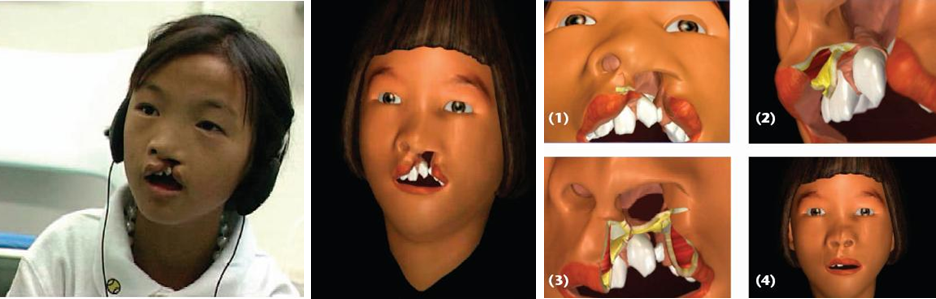
\includegraphics[width=\textwidth]{images/cleft_lip_image}
\caption{Surgical simulation will ideally be used to provide a virtual environment of prototyping procedures as well as for research and development of novel procedures. The images show a subject specific simulated cleft lip and palate repair. Elastic simulation of soft tissues is the primary algorithmic challenge in providing such technologies.}
\label{fig:cleft_lip}
\end{figure}

\section*{Real-time computing}
Real-time simulation refers to the ability to evolve the approximation to an initial boundary value problem in less than a thirtieth of a second. In other words, less than the time it would take to observe the solution on the screen. Traditionally, computation times required for a time step in such problems have been on the order of a few minutes or even a few hours, far short of the thirtieth of a second constraint. However, such performance, should it be allowed, would provide a controllable virtual environment where a user would have the ability to change the forcing and boundary conditions of a simulation in response to real-time observation of the solution. The availability of such functionality for problems in solid and fluid mechanics engenders many new opportunities and applications. For example, imagine an interactive virtual environment where the user interacts with a finite element simulation of biomechanical soft tissues. The governing equations dictate how the tissues respond to external influence from the users. This predictive ability would allow the user to push, pull or even cut/excise portions of the tissue in real time with full confidence that the real life counterpart would behave similarly. This ability could potentially revolutionize the process of training surgical residents and medics by providing a cost effective and scientific alternative to expensive cadaver based training. Imagine the ability to know the outcome of a surgical procedure before it is performed. Reconstructive surgery for severe trauma is unpredictable by the nature of the injuries. The surgeon must design the treatment procedure on a case-by-case basis. With the aid of a predictive simulator the surgeon could perform hypothetical surgical repairs in advance to determine the most likely successful approach. This would significantly reduce complication rates and lead to drastically improved quality of life. See \cite{Sifakis09} for further discussion of the potential benefits of surgical simulation.

%%%%%%%%%%%%%%%%%%%%%%%%%%%%%%%%%%%%%%%%%%%%%%%%%%%%%%%%%%%%%%%%%%%%%%%%%%%%%%%%
% partI/partI.tex
%
% Copyright 2012, Jeffrey Hellrung.
%%%%%%%%%%%%%%%%%%%%%%%%%%%%%%%%%%%%%%%%%%%%%%%%%%%%%%%%%%%%%%%%%%%%%%%%%%%%%%%%

\part{Applications of Arbitrary Lagrangian Mesh Cutting}

\renewcommand{\thechapter}{\thepart}

\section*{Introduction}

Many physical simulations necessitate the modeling of fracture or crack surfaces, and in the most demanding of these simulations, these surfaces may have a highly complex non-manifold topology, e.g., with many branches and open ``fronts''. In a dynamics scenario, this may be further complicated by the frequent extension of existing crack fronts and the introduction of new failure surfaces. Applying a traditional finite element method in this context is challenging: one must either constantly regenerate the simulation mesh to account for the fracture geometry, which is computationally expensive and easily introduces ill-conditioned ``sliver'' elements; or one must artificially and often severely limit the potential paths and resolution of the failure surface to lie along element boundaries. Additionally, in either case, handling a high resolution fracture surface necessitates a correspondingly high resolution simulation volume, at least locally, which in turn increases the computational cost of solving the relevant discretized continuum mechanics equations. Ideally, one should be able to decouple the resolution of the fracture surface (which may be highly detailed for visual effects purposes, for example; see Chapter~\ref{chap:partI.fractureanimation}) from the resolution of the simulation mesh (which may be limited by available computational resources; see Chapter~\ref{chap:partI.virtualsurgery}).

Given the above difficulties with traditional finite element methods, Belytschko, Black, Mo\"{e}s, Dolbow \cite{Belytschko99, Moes99} and others developed the \emph{eXtended Finite Element Method} (XFEM), which avoids the need to remesh to capture crack geometry. The basic idea of the XFEM is to enrich the usual finite element spaces with additional degrees of freedom which incorporate the near tip asymptotic solutions and allow the displacements around the crack surface to be discontinuous. We hold off a complete introduction to and history of the XFEM until Chapter~\ref{chap:partI.crackpropagation}, but do mention one of the main challenges with utilizing the XFEM: automating the determination of material connectivity and subsequent enrichment of the finite element spaces. In the following chapters, we apply the mesh cutting algorithm of Sifakis et al. \cite{Sifakis07} to resolve arbitrary Lagrangian cutting surfaces against the simulation volume mesh, determine material connectivity, and automatically duplicate mesh vertices to yield \emph{virtual nodes} which effect the requisite enrichment necessary for crack separation.

We conclude this prelude to Part I with a brief summary of the mesh cutting algorithm from \cite{Sifakis07}, as the main subject of Part I is the various applications of this algorithm. Chapter~\ref{chap:partI.crackpropagation} combines the XFEM with the mesh cutting algorithm to simulate propagating cracks in $2$ dimensions; we also introduce a novel quadrature scheme to accurately and straightforwardly integrate the nonlinear and singular finite element basis functions. In Chapter~\ref{chap:partI.virtualsurgery}, we consider the combination of this mesh cutting algorithm with nonlinear continuum mechanics in $3$ dimensions to create a virtual surgery simulator. Lastly, in Chapter~\ref{chap:partI.fractureanimation}, we discuss a framework to systematically create cracked and shattered models for use in computer animation.

\section*{Mesh Cutting Algorithm Overview}

We now give a brief overview of the mesh cutting algorithm described by Sifakis et al.; see \cite{Sifakis07} for more details, specifically in resolving the intra-simplex geometry, the discussion of which we exclude here. The essence of the algorithm may be described by considering the resolution of a segmented curve cutting surface against a triangulated area as the volumetric mesh, although the following overview applies equally well to higher dimensions (as seen in Chapters~\ref{chap:partI.virtualsurgery} and \ref{chap:partI.fractureanimation}, for example). Ultimately, the algorithm produces a geometrically coincident volumetric mesh with mesh elements along the cutting surface duplicated into materially disconnected counterparts; see Figure~\ref{fig:partI.cutting.example} for an example overview of the entire procedure.

\setlength{\figurewidth}{\textwidth}
\begin{figure}[htb]
\centering
\includegraphics[width=\figurewidth]{partI/figures/cutter_illustration}
\caption{This mesh is cut by two curves, one of which contains a branch (left). The cutting algorithm first treats each triangle individually, creating duplicates for each locally disjoint material region (center), and then uses the global mesh topology to join these duplicates on the proper degrees of freedom (right). }
\label{fig:partI.cutting.example}
\end{figure}

In the first phase, the algorithm processes each mesh triangle individually, identifying the disjoint \emph{material components} the triangle is divided into by the cutting curve and describing each as a closed polygonal region (depicted blue in Figure~\ref{fig:partI.cutting.triangle.2}). For each such material region, a duplicate copy of the triangle is created and assigned said material region. For example, in Figure~\ref{fig:partI.cutting.triangle.2}, the cutting curve divides the triangle into two distinct material regions, inducing the creation of two duplicates of the original triangle with each duplicate possessing one of the material regions. In the duplicated triangles, we identify vertices within material regions (solid blue circles in Figure~\ref{fig:partI.cutting.triangle.2}) with the original triangle vertices. We also furnish the duplicate triangles with \emph{virtual nodes} (hollow blue circles in Figure~\ref{fig:partI.cutting.triangle.2}). A less trivial example is given in Figure~\ref{fig:partI.cutting.triangle.3}.

\setlength{\figureheight}{0.25\textwidth}
\begin{figure}[htb]
\centering
\includegraphics[height=\figureheight]{partI/figures/cutting}
\caption{Simple example of an original mesh triangle (left) duplicated with its disjoint \emph{material regions} (blue) being distributed among the duplicates (middle, right). Likewise, the vertices in each duplicate are either identified with the vertices of the original triangle (\emph{material nodes}, sold blue) or duplicate copies (\emph{virtual nodes}, hollow blue), depending on whether they fall within a material region.}
\label{fig:partI.cutting.triangle.2}
\end{figure}
\begin{figure}[htbp]
\centering
\includegraphics[height=\figureheight]{partI/figures/complex_cutting}
\caption{A more complex example of the initial division of triangle by a cutting curve. Since the original mesh triangle is divided into $3$ disjoint material regions (left), the algorithm generates $3$ duplicate triangles, each possessing a different material region (right). (Coloring is consistent with that used in Figure~\ref{fig:partI.cutting.triangle.2}.)}
\label{fig:partI.cutting.triangle.3}
\end{figure}

After processing all triangles in the original mesh $\calT$ individually, we obtain a duplicate mesh $\calT'$ composed of duplicate triangles. The second phase of the algorithm proceeds to determine global material connectivity within this duplicate mesh (see Figure~\ref{fig:partI.cutting.example}). For notational convenience, let $C(T)$ denote the set of triangles duplicated from original triangle $T \in \calT$, and let $P(T')$ denote the original ``parent'' triangle of a duplicate triangle $T' \in \calT'$, so that $T' \in C(T)$ if and only if $T = P(T')$. Determining global material connectivity then proceeds as follows. Given a triangle $T' \in \calT'$, let $T = P(T')$. Then for each $U' \in C(U)$ where $U$ is face-adjacent to $T$, determine if $U'$ shares \emph{material connectivity} across the $T-U$ face with $T'$. If so, the vertices of the corresponding faces of $T'$ and $U'$ are identified as equivalent and collapsed, thus joining these duplicate triangles together.

Refer again to Figure~\ref{fig:partI.cutting.example} for an example overview of the entire algorithm. The original mesh, at left, consists of three triangles. This mesh is cut by two segmented curves (red); the geometry typifies some of the subtleties in the algorithm, as the center triangle contains a branch, a tip, and is cut into multiple pieces. In the first phase of the algorithm, each triangle is processed in isolation and duplicated based on the disjoint material regions created by the cutting curves, as shown in the center of Figure~\ref{fig:partI.cutting.example}. In the second phase, these duplicate triangles are joined along faces where they share material connectivity, with the final mesh on the right of Figure~\ref{fig:partI.cutting.example}.

Notice that, in particular, if mesh vertices are identified with degrees of freedom, the latter mesh in Figure~\ref{fig:partI.cutting.example} possesses the necessary richness in degrees of freedom to allow the upper crack to partially separate and the lower crack to separate entirely. This automatic generation of additional degrees of freedom is one of the motivating conveniences to combine this mesh cutting algorithm with an XFEM framework, and its fruits are demonstrated in the remainder of Part I.

\renewcommand{\thechapter}{\arabic{chapter}}

%%%%%%%%%%%%%%%%%%%%%%%%%%%%%%%%%%%%%%%%%%%%%%%%%%%%%%%%%%%%%%%%%%%%%%%%%%%%%%%%
% chapters/chapter1.tex
%
% Copyright 2012, Jeffrey Hellrung.
%%%%%%%%%%%%%%%%%%%%%%%%%%%%%%%%%%%%%%%%%%%%%%%%%%%%%%%%%%%%%%%%%%%%%%%%%%%%%%%%

\chapter{Virtual Surgery}

[TODO]

%%%%%%%%%%%%%%%%%%%%%%%%%%%%%%%%%%%%%%%%%%%%%%%%%%%%%%%%%%%%%%%%%%%%%%%%%%%%%%%%
% part1/chapter2/chapter2.tex
%
% Copyright 2012, Jeffrey Hellrung.
%%%%%%%%%%%%%%%%%%%%%%%%%%%%%%%%%%%%%%%%%%%%%%%%%%%%%%%%%%%%%%%%%%%%%%%%%%%%%%%%

\chapter{Virtual Surgery} \label{ch:pt1.virtualsurgery}

[TODO]

%%%%%%%%%%%%%%%%%%%%%%%%%%%%%%%%%%%%%%%%%%%%%%%%%%%%%%%%%%%%%%%%%%%%%%%%%%%%%%%%
% part1/chapter3/chapter3.tex
%
% Copyright 2012, Jeffrey Hellrung.
%%%%%%%%%%%%%%%%%%%%%%%%%%%%%%%%%%%%%%%%%%%%%%%%%%%%%%%%%%%%%%%%%%%%%%%%%%%%%%%%

\chapter{Geometric Fracture Modeling in Computer Animation} \label{chap:partI.fractureanimation}

[TODO]

%%%%%%%%%%%%%%%%%%%%%%%%%%%%%%%%%%%%%%%%%%%%%%%%%%%%%%%%%%%%%%%%%%%%%%%%%%%%%%%%
% partII/partII.tex
%
% Copyright 2012, Jeffrey Hellrung.
%%%%%%%%%%%%%%%%%%%%%%%%%%%%%%%%%%%%%%%%%%%%%%%%%%%%%%%%%%%%%%%%%%%%%%%%%%%%%%%%

\part{Virtual Node Methods for Elliptic Problems}

\renewcommand{\thechapter}{\thepart}

\section*{Introduction}

We now turn toward the solution of elliptic partial differential equations on arbitrary, irregular domains with a discretization based on a regular Cartesian grid. We will specifically consider the following problems in Chapters~\ref{chap:partII.poisson} and \ref{chap:partII.LE}, respectively.

\begin{itemize}

\item Poisson's equation with interfacial jump conditions:
\begin{subequations} \label{eq:partII.poisson}
\begin{align}
-\nabla \cdot \lrp{\beta \nabla u} & = f, \quad \in \Omega \setminus \Gamma; \label{eq:partII.poisson.PDE} \\
\jump{u} & = a, \quad \in \Gamma; \label{eq:partII.poisson.DJ} \\
\jump{\beta \nabla u \cdot \hatn} & = b, \quad \in \Gamma; \label{eq:partII.poisson.NJ} \\
u & = p, \quad \in \dOmega_d; \label{eq:partII.poisson.D} \\
\beta \nabla u \cdot \hatn & = q, \quad \in \dOmega_n; \label{eq:partII.poisson.N}
\end{align}
\end{subequations}
where
\begin{itemize}
\item the domain $\Omega \subset \bbR^d$ is open ($d = 2 \text{ or } 3$, typically);
\item the interface $\Gamma$ is a co-dimension one closed curve ($d = 2$) or surface ($d = 3$) that divides $\Omega$ into an interior domain $\Omega^-$ and an exterior domain $\Omega^+$, such that $\Omega = \Omega^- \sqcup \Omega^+ \sqcup \Gamma$;
\item $u$ (unknown), $\beta$ (known), and $f$ (known) are scalar functions which can exhibit discontinuities across $\Gamma$ but otherwise are assumed to have smooth restrictions $u^{\sigma}$, $\beta^{\sigma}, f^{\sigma}$ to $\Omega^{\sigma}$, $\sigma \in \set{+,-}$;
\item $\hatn \equiv \hatn(\bfx)$ denotes the outward unit normal, both to $\Omega^-$ for $\bfx \in \Gamma$ and to $\Omega$ for $\bfx \in \dOmega$; and
\item $\jump{v}(\bfx) := v^+(\bfx) - v^-(\bfx) := \lim_{\epsilon \to 0^+} v\lrp{\bfx + \epsilon \hatn(\bfx)} - \lim_{\epsilon \to 0^+} v\lrp{\bfx - \epsilon \hatn(\bfx)}$ denotes the \emph{jump} of the quantity $v$ across the interface $\Gamma$.
\end{itemize}
We note that the relevant physics generally determine the jumps in the solution \eqref{eq:partII.poisson.DJ} and in the flux \eqref{eq:partII.poisson.NJ}, as well as the boundary conditions \eqref{eq:partII.poisson.D}, \eqref{eq:partII.poisson.N} on $\dOmega$.

\item The equilibrium equations of linear elasticity:
\begin{subequations} \label{eq:partII.elasticity}
\begin{align}
-\nabla \cdot \bssigma(\bfu) & = \bff, \quad \in \Omega; \\
\bfu & = \bfu_0, \quad \in \dOmega_d; \\
\bssigma(\bfu) \cdot \hatn & = \bfg, \quad \in \dOmega_n;
\end{align}
\end{subequations}
where
\begin{itemize}
\item the domain $\Omega \subset \bbR^d$ is open (we consider $d = 2$ primarily);
\item $\bfu$ is the (unknown) material displacement map;
\item $\bssigma$ is the Cauchy stress tensor;
\item $\bff$ is the external force per unit volume;
\item $\bfu_0$ is the prescribed Dirichlet boundary displacements over $\dOmega_d \subset \dOmega$; and
\item $\bfg$ is the prescribed external surface traction over $\dOmega_n \subset \dOmega$.
\end{itemize}
In linear elasticity, the stress $\bssigma(\bfu)$ is linearly dependent on the Cauchy strain $\bsepsilon(\bfu)$ via
\begin{align*}
\bsepsilon(\bfu) := {} & \frac{1}{2} \lrp{\nabla \bfu + \lrp{\nabla \bfu}^t}, \\
\bssigma(\bfu)   := {} & 2 \mu \bsepsilon(\bfu) + \lambda \lrp{\tr \bsepsilon(\bfu)} \bfI \\
                  = {} & \mu \lrp{\nabla \bfu + \lrp{\nabla \bfu}^t} + \lambda \lrp{\nabla \cdot \bfu} \bfI.
\end{align*}
Therefore, \eqref{eq:partII.elasticity} is equivalently formulated as
\begin{subequations} \label{eq:partII.LE}
\begin{align}
-\lrp{\mu \Delta \bfI + (\lambda + \mu) \nabla \nabla^t} \bfu & = \bff \quad \in \Omega \label{eq:partII.LE.PDE} \\
\bfu & = \bfu_0 \quad \in \dOmega_d \label{eq:partII.LE.D} \\
\mu \lrp{\bfu \cdot \hatn + \nabla \lrp{\bfu \cdot \hatn}} + \lambda \lrp{\nabla \cdot \bfu} \hatn & = \bfg \quad \in \dOmega_n \label{eq:partII.LE.N}.
\end{align}
\end{subequations}

\end{itemize}

In all the above, $\dOmega = \dOmega_d \sqcup \dOmega_n$, and we assume $\Gamma$ (if applicable) and $\dOmega$ to be sufficiently smooth. See Figure~\ref{fig:partII.embedding} for an example of an embedding of a domain $\Omega$ within a background Cartesian grid in $2$ and $3$ dimensions.

\setlength{\figureheight}{0.50\textwidth}
\begin{figure}[htb]
\centering
\subfloat[Embedding in $2$ dimensions]
{\includegraphics[height=\figureheight]{partII/figures/embedding_2d}}
\subfloat[Embedding in $3$ dimensions]
{\includegraphics[height=\figureheight]{partII/figures/embedding_3d}}
\caption{Example domain embeddings in (a) $2$ dimensions and (b) $3$ dimensions. In a typical domain embedding, only grid vertices on grid cells which intersect the domain (in (a), shaded) are considered degrees of freedom.}
\label{fig:partII.embedding}
\end{figure}

Although the use of embedded methods avoids the complexities inherent to unstructured mesh generation, as discussed in the overall Introduction, they do introduce difficulties of their own, though typically of a different and less computationally intensive variety. One prominent such difficulty is the enforcement of algebraic surface conditions (such as boundary conditions or interfacial jump conditions) on embedded features such as $\dOmega$ and $\Gamma$, since the degrees of freedom now do not lie on said embedded features. Our methods employ a Lagrange multiplier space in a relatively straightforward way to weakly enforce Dirichlet boundary conditions and interfacial jump conditions. We mention some alternative techniques in the background sections in the subsequent chapters, and for a good review, see Lew et al. \cite{Lew.Adrian08}.

A further challenge is the retention of higher order accuracy in $L^{\infty}$. The difficulty typically lies in determining the numerical stencils near embedded features that retain the accuracy achieved in the regions of the domain sufficiently distanced from embedded features. Many present methods address these problems at the cost of implementation complexity and sometimes require significant effort to adapt to general applications. But while achieving higher order accuracy in the discretization may be nontrivial, to reiterate from the overall Introduction, the ability to use a regular Cartesian grid greatly facilitates the implementation of efficient solution techniques. Specifically for high resolution discretizations, direct methods to solve the discrete linear systems become too slow and memory intensive. Geometric multigrid methods and domain decomposition approaches have been shown to provide very favorable performance in this setting. However, their application to embedded discretizations is not entirely straightforward. Ultimately, special attention must be paid near embedded features for both discretization accuracy and efficient numerical linear algebra, as we describe in the subsequent chapters.

The methods presented in the following chapters build on the work of Bedrossian et al. \cite{Bedrossian10}, which introduced a second order virtual node method for solving the interfacial Poisson problem \eqref{eq:partII.poisson} in $2$ dimensions. The discretization presented in \cite{Bedrossian10} is easy to implement and yields a symmetric positive definite sparse linear system for both interface problems and boundary value problems on irregular domains. In summary, this virtual node method employs a uniform Cartesian grid with duplicated Cartesian bilinear elements along the interface. These duplicated elements introduce additional \emph{virtual} nodes or degrees of freedom to accurately capture the lack of regularity in the solution. The method is variational to define stencils symmetrically, and a different discretization is used depending on proximity to embedded features, allowing for the retention of the standard $5$-point finite difference stencil away from embedded boundaries and interfaces. Langrange multipliers are used to weakly enforce embedded Dirichlet conditions \eqref{eq:partII.poisson.D} and embedded interfacial jump conditions \eqref{eq:partII.poisson.DJ}, and the choice of Lagrange multiplier space admits a symmetric positive definite discretization. In the special case when $\beta$ is smooth, a discontinuity removal technique allows the use of the standard $5$-point Poisson stencil even across the embedded interface.

In Chapter \ref{chap:partII.poisson}, we improve many aspects of \cite{Bedrossian10} and provide key modifications necessary to extend the method to $3$ dimensions. Within the context of discretizing the Dirichlet conditions \eqref{eq:partII.poisson.D} and interfacial jump conditions \eqref{eq:partII.poisson.DJ}, we present a novel and flexible algorithm to define the discrete Lagrange multiplier space. This algorithm gives more control on the conditioning of the resulting linear system and specifically addresses the conditioning issues (see Appendix~\ref{chap:partII.appendix.constraintconditioning}) we found in the straightforward extension of \cite{Bedrossian10} to $3$ dimensions. We also give an expanded treatment of the discontinuity removal technique, detailing an algorithm for the construction of a scalar function satisfying the interfacial jump conditions (\ref{eq:partII.poisson.DJ}, \ref{eq:partII.poisson.NJ}).

In Chapter \ref{chap:partII.LE}, we apply some of the same basic ideas from Chapter \ref{chap:partII.poisson} to numerically solve the equilibrium equations of linear elasticity in the nearly incompressible regime. We stabilize the method by introducing pressure as an additional unknown in a mixed variational formulation. Our discretization of this variational formulation is then based on a MAC-type staggering of $x$ and $y$-component displacements with pressure degrees of freedom at cell centers. Again, we achieve second order accuracy in $L^{\infty}$ while retaining a symmetric positive definite linear system.

Further, within both chapters, we present a family of geometric multigrid algorithms to solve the resulting linear systems with near-optimal multigrid efficiency independent of grid resolution. The variational nature of the methods naturally enables symmetric numerical stencils along embedded features, and together with our choice of Lagrange multiplier space, this admits an efficient means for smoothing boundary and interface equations. Indeed, this shows the suitability of efficient parallel implementations, as indicated, e.g., by the similarities to the first order method to solve \eqref{eq:partII.LE} in \cite{Zhu.Yongning10}.

In summary, our methods for solving elliptic problems such as Poisson's equation \eqref{eq:partII.poisson} and the equilibrium equations of linear elasticity \eqref{eq:partII.LE} have a distinguishing feature set rarely found simultaneously in the large class of embedded methods:
\begin{itemize}
\item second-order accuracy in $L^{\infty}$;
\item addresses both Neumann \eqref{eq:partII.poisson.N} / \eqref{eq:partII.LE.N} and Dirichlet \eqref{eq:partII.poisson.D} / \eqref{eq:partII.LE.D} boundary conditions as well as the interfacial jump conditions (\ref{eq:partII.poisson.DJ}, \ref{eq:partII.poisson.NJ});
\item relatively simple to implement with a nice progression of complexity from the discretization of Neumann boundary conditions to Dirichlet boundary conditions to interfacial jump conditions;
\item yields a discrete linear system which is symmetric and positive definite, facilitating the application of a wide variety of black-box solvers or, as we show, efficient geometric multigrid methods with nearly optimal convergence rates.
\end{itemize}
Furthermore, our method for solving \eqref{eq:partII.LE} retains the above properties even in the nearly incompressible regime.

\renewcommand{\thechapter}{\arabic{chapter}}

%%%%%%%%%%%%%%%%%%%%%%%%%%%%%%%%%%%%%%%%%%%%%%%%%%%%%%%%%%%%%%%%%%%%%%%%%%%%%%%%
% part2/chapter4/chapter4.tex
%
% Copyright 2012, Jeffrey Hellrung.
%%%%%%%%%%%%%%%%%%%%%%%%%%%%%%%%%%%%%%%%%%%%%%%%%%%%%%%%%%%%%%%%%%%%%%%%%%%%%%%%

\chapter{Poisson with Interfacial Jump Conditions} \label{ch:pt2.poisson}

\section{Background and Existing methods} \label{sec:ch4.background}

\footnote{The content of this chapter is largely a revision of \cite{Hellrung12}.}
To review, this chapter addresses the solution of Poisson's equation with interfacial jump conditions, repeated here for convenience:
\begin{subequations} \label{eq:ch4.poisson}
\begin{align}
-\nabla \cdot \lrp{\beta \nabla u} & = f, \quad \in \Omega \setminus \Gamma; \label{eq:ch4.poisson.PDE} \\
\jump{u} & = a, \quad \in \Gamma; \label{eq:ch4.poisson.DJ} \\
\jump{\beta \nabla u \cdot \hatn} & = b, \quad \in \Gamma; \label{eq:ch4.poisson.NJ} \\
u & = p, \quad \in \dOmega_d; \label{eq:ch4.poisson.D} \\
\beta \nabla u \cdot \hatn & = q, \quad \in \dOmega_n; \label{eq:ch4.poisson.N}
\end{align}
\end{subequations}
where we wish to solve for the unknown scalar function $u$.

The \emph{Immersed Interfaced Method} (IIM) is perhaps the most popular finite difference method for approximating \eqref{eq:ch4.poisson} to second order accuracy. LeVeque and Li first proposed the IIM for approximating elliptic interface problems in \cite{Leveque94} and the term now applies to a widely researched and extensively applied class of finite difference methods \cite{Leveque97, Li.Zhilin01b, Lee.Long03, Le.DV06, Xu.Sheng06, Tan.Zhijun08, Xu.Sheng08}. See \cite{Li.Zhilin06a} and the references therein for a complete exposition of the method and its numerous applications, and \cite{Beale06} for justification of the general IIM approach. Using generalized Taylor expansions, the original IIM adaptively modifies the stencil to obtain $\calO(h)$ truncation error along the interface. For smooth $\beta$, this reduces to the standard $5$-point or $7$-point finite difference stencil, but otherwise results in an asymmetric discretization that follows from locally solving constrained optimization problems that enforce a discrete maximum principle \cite{Li.Zhilin01a}. The IIM also generally requires the evaluation of higher order jump conditions and surface derivatives along the interface. This can lead to difficulty in implementation, especially in $3$ dimensions \cite{Deng03, Li.Zhilin06a, Xu.Sheng06, Xu.Sheng08}. Chen and Strain described a new approach to the IIM, called the \emph{Piecewise-polynomial Interface Method} (PIM), in \cite{Chen.Tianbing08} that does not require the derivation of additional jump conditions and accurately treats complex interfaces. Various other attempts have been made \cite{Li.Zhilin98a, Weigmann00, Berthelsen04, Adams.Loyce02, Adams.Loyce04, Adams.Loyce05, Li.Zhilin06a} to improve the efficiency and reduce the complexity of the IIM.

Extrapolation-based finite difference schemes such as \cite{Liu.Xu-Dong00, Gibou02, Zhou.YC06a, Gibou05, Jomaa05, Chern07} introduce fictitious points along coordinate axes and use the known jump conditions to determine their values. The \emph{Ghost Fluid Method} (GFM), such as that presented by Liu et al. in \cite{Liu.Xu-Dong00}, exemplifies such methods. For $2-$ and $3-$dimensional interface problems, the GFM neglects the tangential flux terms $\jump{\beta \nabla u \cdot \hat{\mathbf{\tau}}}$ when determining fictitious values, yielding a symmetric positive definite system and a resulting method which is first order accurate \cite{Liu.Xu-Dong00, Liu.Xu-Dong03}. However, the GFM is capable of achieving up to fourth order accuracy for irregular domain problems \cite{Gibou02, Gibou05}. The GFM is similar to our approach in spirit. We also incorporate similar ideas from the \emph{Virtual Node Algorithm} (VNA) \cite{Molino05, Bao.Zhaosheng07, Sifakis07}. Various other approaches attain higher order accuracy by accounting for the tangential flux in other ways, often sacrificing simplicity and symmetry of discretization in the process. For instance, the \emph{Coupling Interface Method} (CIM) \cite{Chern07} extends the GFM to higher order by using a second order extension at most grid points but reverting to a first order method at grid points where the second order extension cannot be applied. The method couples jump conditions in different directions to express the tangential derivatives, and the use of one-sided differences results in an asymmetric discretization. Similarly, the \emph{Matched Interface and Boundary \textnormal{(MIB)} method} \cite{Zhou.YC06a} uses higher order extrapolations of the solution matched with higher order one-sided discretizations of the jump conditions to determine the values at fictitious points. The MIB method accounts for nonzero $\jump{\beta \nabla u \cdot \hat{\mathbf{\tau}}}$ by differentiating the given jump conditions using one-sided interpolations. This widens the stencil in several directions that depend on the local geometry, and results in an asymmetric discretization. The work of \cite{Zhou.YC06b} extended the MIB method to handle high curvature geometry, the work of \cite{Yu.Sining07} provides a $3$-dimensional version, and more recent progress is given in \cite{Zhao.Shan09}. Kejia Pan et al. in \cite{Pan.Kejia10} derived symmetric finite difference formulas (in $1$ and $2$ dimensions) within the MIB framework. In \cite{Hou.Songming05,Hou.Songming10} Hou et al. also use techniques seemingly inspired by the analysis of the original GFM approach done in \cite{Liu.Xu-Dong00,Liu.Xu-Dong03}. They develop a second order variational GFM by altering finite element interpolating functions to capture the jump conditions in the solution. Their approach is remarkably robust to non-smooth interface geometry (especially \cite{Hou.Songming10}), but results in an asymmetric discretization in the general case. The recent works of \cite{Ng.YenTing09, Papac10} treated the cases of Robin and Neumann boundary conditions by altering the $5$-point stencil along the boundary using a finite volume-like approach. This results in a symmetric positive definite system.

Ideas similar to the extrapolation-based finite difference schemes have also seen extensive use in the FEM community, for instance in fictitious domain methods \cite{Glowinski94a, Almgren97, Parussini09, Jomaa10}, the \emph{Discontinuous Galerkin \textnormal{(DG)} method} \cite{Lew.Adrian08, Guyomarch09}, the \emph{eXtended Finite Element Method} (XFEM) \cite{Moes99, Daux00, Belytschko01, Moes03, Ji.H.04, Fries06, Moes06, Groi07, vanderBos09} \cite{Vaughan06}\footnote{See \cite{Beale08} for corrections to IIM convergence estimates.}, and other non-conforming finite element methods \cite{Young.DavidP.90, Hansbo02, Li.Zhilin03, Hansbo04, Song06, Mourad07, Dolbow08, Kumar08, Dolbow09, Harari10, Kwak.DoY10, Wu.Haijun10}. Fictitious domain methods handle embedded features by including every element that intersects the feature into the discretization. This naturally introduces ``virtual nodes'' or ``ghost nodes'' into the resulting discretization. The XFEM enriches the standard finite element basis with additional discontinuous basis functions, thereby introducing new degrees of freedom. These basis functions exist only at the nodes of elements that intersect the embedded interface and usually are the standard basis elements multiplied by a generalized Heaviside function. The methods of \cite{Hansbo02, Hansbo04, Song06, Bao.Zhaosheng07, Dolbow09} introduce a related virtual node concept to provide the additional degrees of freedom required to represent the discontinuities. The most straightforward implementation of this virtual node concept \cite{Hansbo04, Song06, Dolbow09} yields a representation equivalent to the standard Heaviside enrichment of the XFEM. However, this approach generalizes to the slightly richer representations of \cite{Molino05, Sifakis07} that attain more geometric detail, particularly when dealing with coarse grids and non-smooth interfaces. Moreover, virtual node representations are considered more geometrically intuitive and easier to incorporate into existing FEM code \cite{Song06, Dolbow09} than traditional Heaviside enrichment.

The solution spaces of these FEM approaches generally do not satisfy the embedded boundary or interface conditions. Thus, these methods impose linear constraints with either penalty methods or Lagrange multipliers to enforce the conditions in some weak sense. For example, see \cite{Glowinski94a, Mourad07, Dolbow09, Parussini09, vanderBos09} and the references therein. When using Lagrange multipliers, the Ladyzhenskaya-Babu\u{s}ka-Brezzi inf-sup conditions place stringent limitations on the types of constraints that will retain optimal convergence rates of the approximation spaces \cite{Babuska73, Pitkaranta79, Chapelle93, Moes06, Mourad07, Lew.Adrian08}. Such inf-sup restrictions generally limit the strength of the Lagrange multiplier space relative to the solution approximation space. For certain elements, designing the proper approximation spaces is a non-trivial task \cite{Ji.H.04,Moes06}. Moreover, the use of Lagrange multipliers requires the solution of an indefinite saddle point system that can potentially introduce significant cost. Applying stabilization through a consistent penalty method, such as Nitsche's method, presents an alternative approach \cite{Hansbo04, Mourad07, Dolbow08, Dolbow09, Harari10, Wu.Haijun10}. However, these can have adverse effects on conditioning and require the determination of the stabilization parameters. Instead of using Lagrange multipliers or stabilization, the methods of \cite{Li.Zhilin03, Hou.Songming05, Fries06, Li.Zhilin98b, Kumar08, Hou.Songming10, Kwak.DoY10} alter the basis functions to either satisfy the constraints directly, or simplify the process of doing so. In this regard, such methods represent the finite element analogues of the IIM.

The method of \cite{Johansen98} offers a finite volume approach to embedded domain problems. Like some fictitious domain methods, XFEM, and our virtual node method, this method uses partially empty cells along the boundary. However, the one-sided quadratic interpolations used to compute the fluxes along the boundary yield an asymmetric system. See \cite{Schwartz06} and \cite{Crockett10} for a more recent $3$-dimensional version applied to Poisson's equation and the heat equation. In \cite{Oevermann06}, Oevermann and Klein proposed a second order finite volume method for interface problems, and simplified and extended their method to $3$-dimensions in \cite{Oevermann09}. In an approach similar to ours, any Cartesian cell that intersects the interface yields a distinct multilinear representation of the solution. The jump conditions are then built into the difference stencil by locally solving constrained overdetermined systems. An asymptotic technique resolves the problem of vanishing cell volumes, though it requires specific treatment for each possible cell geometry. The resulting system is asymmetric for the general case of $\jump{\beta} \neq 0$.

When $\jump{\beta} \neq 0$ the majority of these second order methods do not retain a symmetric positive definite system. While the FEM approaches that use stabilization do retain a symmetric positive definite system \cite{Dolbow09}, generally the finite element methods that use Lagrange multipliers, such as \cite{Daux00}, result in a symmetric indefinite system. Although we use Lagrange multipliers, we present a simple method of reducing the indefinite system to a symmetric positive definite system using a null space method. On the other hand, when the coefficient $\beta$ is smooth across the interface, methods such as the original IIM achieve second order accuracy by only altering the right-hand side of the system. For this case, we present a method that uses the virtual node framework that also retains the original left-hand side.

Several of the above works employ multigrid methods to solve the resulting linear systems. Black-box multigrid solvers, either of a purely algebraic variety \cite{Deng03, Oevermann06, Chern07, Oevermann09} or of a more geometric variety \cite{Li.Zhilin01a}, are often efficient alternatives to, or may be combined with, Krylov solvers \cite{Chen.Tianbing08, McAdams10}. However, less general multigrid algorithms specially tuned to the particular discretization method may outperform a black-box multigrid solver; see, for example, \cite{Adams.Loyce05, McAdams10}. Some methods lend themselves to using relatively straightforward extensions of standard geometric multigrid techniques, including both mortar finite element methods \cite{Wohlmuth99, Lamichhane04} and embedded methods \cite{Almgren97, Johansen98, Schwartz06, Crockett10}, usually with special attention being paid near irregular features. Many of the works describing IIM-based discretizations \cite{Adams.Loyce02, Adams.Loyce04, Adams.Loyce05, Chen.Tianbing08} utilize a multigrid solver with a grid hierarchy defined geometrically but incorporate algebraic techniques in the remaining components (coarse-grid operators and grid transfer operators). In \cite{Wan.Justin04} Wan and Liu discuss the transfer operators near embedded features in a geometric multigrid method for irregular domain discretizations in general. In contrast to the multigrid approaches in many of the preceding works on embedded discretizations, our multigrid algorithms define the grid hierarchy, coarse-grid operators, and grid transfer operators geometrically, hence allow for efficient implementations that have lower memory requirements and increased parallelizability.

\section{Discretization} \label{sec:ch4.discretization}

Our numerical discretizations for domain and interface problems make use of an embedding of the domain boundary and/or interface within a uniform Cartesian grid. We thus first outline this embedding procedure and the associated notation. We subsequently describe our Neumann discretization, and we will then see how an alteration of our treatment of the boundary conditions in Neumann problems yields our discretization for Dirichlet problems. Finally, we will show how a natural combination of our Neumann and Dirichlet discretizations allows us to deal with interfacial discontinuities.

\subsection{Domain and Interface Embedding and Integration} \label{subsec:ch4.discretization.embedding}

Let us first consider the treatment of $\Omega$ for domain problems. We embed the domain $\Omega$ into a non-conforming, uniform Cartesian grid $\calG^h$ with grid-spacing $(\Delta x, \Delta y, \Delta z)$. (Note that to simplify the convergence analysis, our numerical examples assume $\Delta x = \Delta y = \Delta z =: h$.) We include all Cartesian grid cells $c_i$ that intersect $\Omega$ in the discretization, and refer to this set $\calC^h = \set{ c_i \in \calG^h : c_i \cap \Omega \neq \emptyset }$ as the \emph{computational domain} (see Figure~\ref{fig:ch4.embedding.domain}). Also, we define the set of all cells that intersect the boundary as $\calC_{\dOmega}^h = \set{ c_i \in \calC^h : c_i \cap \dOmega \neq \emptyset }$ and refer to these as \emph{boundary (grid) cells}. Note that a boundary cell may be regarded as partially empty, since only a portion of the cell lies within $\Omega$. We refer to this region of a boundary cell $c_i$ that lies in the domain $\Omega$, $c_i \cap \Omega$, as the \emph{material region} of the cell, and use the terms \emph{material node} and \emph{virtual node} to describe the Cartesian grid vertices lying inside and outside $\Omega$, respectively. We refer to the set of grid vertices spanned by the computation domain as $\calN^h$, and specifically the material nodes as $\calN^h_m$ and the virtual nodes as $\calN^h_v$. See Figure~\ref{fig:ch4.embedding.domain} for a diagram labeling the grid vertices along a typical boundary. For domain problems, we identify each grid vertex in the computational domain, material or virtual, as a degree of freedom.

\setlength{\figureheight}{0.40\columnwidth}
\begin{figure}[htbp]
\begin{center}
\subfigure[Embedding in $2$ dimensions]
{\includegraphics[height=\figureheight]{part2/figures/embedding_2d}}
\subfigure[Embedding in $3$ dimensions]
{\includegraphics[height=\figureheight]{part2/figures/embedding_3d}}
\caption{Example embeddings for domain problems. Subfigure (a) shows an example in $2$ dimensions to clearly depict the various classes of grid cells and vertices: shaded grid cells comprise the computational domain ($\calC^h$), with lighter-shaded grid cells on the boundary ($\calC_{\dOmega}^h$); grid vertices surrounded by gray circles represent virtual degrees of freedom ($\calN^h_v$); grid vertices surrounded by black circles represent material degrees of freedom ($\calN^h_m$) incident to a boundary grid cell; and grid vertices surrounded by squares represent material degrees of freedom ($\calN^h_m$) incident only to non-boundary grid cells. Subfigure (b) shows an example in $3$ dimensions.}
\label{fig:ch4.embedding.domain}
\end{center}
\end{figure}

In the course of the discretization, for each boundary cell $c_i \in \calC_{\dOmega}^h$, we will need to evaluate integrals over the following domains:
\begin{itemize}
\item the material volume within a cell, $c_i \cap \Omega$;
\item the boundary of the material volume within a cell, $\partial(c_i \cap \Omega)$; and
\item the boundary of $\Omega$ within a cell, $c_i \cap \dOmega$ (which is contained within $\partial(c_i \cap \Omega)$).
\end{itemize}
In all cases, the integrand is polynomial (or locally approximated by a polynomial). We evaluate these integrals using polyhedral representations $\calP^{c_i}$ and $\calP_{\dOmega}^{c_i}$ approximating $\partial(c_i \cap \Omega)$ and $c_i \cap \dOmega$, respectively. We use the term \emph{polyhedral representation} to convey an analogous meaning as polygonalizing a curve in $2$ dimensions, but we essentially regard $\calP^{c_i}$ and $\calP_{\dOmega}^{c_i}$ simply as collections of polygons. For implementation purposes, to maximize data structure reuse, it is convenient for $\calP_{\dOmega}^{c_i} \subset \calP^{c_i}$, i.e., all polygons in $\calP_{\dOmega}^{c_i}$ are also members of $\calP^{c_i}$. See Figure~\ref{fig:ch4.boundarypolyhedralization}.

\setlength{\figureheight}{0.32\columnwidth}
\begin{figure}[htbp]
\begin{center}
\subfigure[Boundary grid cell with a polyhedralization of a portion of $\dOmega$ embedded inside]
{\includegraphics[height=\figureheight]{part2/chapter4/figures/boundary_cell_a}}
\subfigure[The two halves of the boundary grid cell after division along $\dOmega$]
{\includegraphics[height=\figureheight]{part2/chapter4/figures/boundary_cell_b}}
\caption{A grid cell $c_i$ with an example boundary dividing it. The left half of the cell in (b) corresponds to $c_i \cap \Omega$, the material region of the cell. (b) shows the polyhedralization $\calP^{c_i}$ of the material region of the cell, where the shaded triangles highlight $\calP_{\dOmega}^{c_i} \subset \calP^{c_i}$, the polyhedralization just of the portion of $\dOmega$ passing through $c_i$.}
\label{fig:ch4.boundarypolyhedralization}
\end{center}
\end{figure}

We employ the divergence theorem to transform volume integrals over $c_i \cap \Omega$ into surface integrals over $\partial(c_i \cap \Omega)$ (cf. \cite{Min.Chohong07}). Such transformations are non-unique, but constructing a simple one is straightforward given the polynomial nature of the integrand. For example,
\begin{align*}
\int_{c_i \cap \Omega} x^p y^q z^r d\bfx
& = \int_{c_i \cap \Omega} \frac{1}{p+1} \nabla \cdot \lrp{x^{p+1} y^q z^r, 0, 0} d\bfx \\
& = \int_{\partial(c_i \cap \Omega)} \frac{1}{p+1} \lrp{x^{p+1} y^q z^r, 0, 0} \cdot \hatn(\bfx) d\bfS(\bfx).
\end{align*}
We decompose surface integrals over $\partial(c_i \cap \Omega)$ and $c_i \cap \dOmega$ into a sum of integrals over the component polygons of $\calP^{c_i}$ and $\calP_{\dOmega}^{c_i}$, respectively. For example, given a vector-valued function $\bfh(\bfx)$,
\begin{equation*}
\int_{\partial(c_i \cap \Omega)} \bfh(\bfx) \cdot \hatn(\bfx) d\bfS(\bfx) = \sum_{g \in \calP^{c_i}} \int_g \bfh(\bfx) \cdot \hatn_g d\bfS(\bfx).
\end{equation*}
Note that over each polygon $g \in \calP^{c_i}$, the unit normal $\hatn_g$ is constant, hence $\bfh(\bfx) \cdot \hatn_g$ restricted to $g$ is a polynomial in $\bfx$ (assuming that the components of $\bfh$ are polynomials to begin with). To evaluate these polygon-local surface integrals, one could make a change of variables into a localized coordinate system and again apply the divergence theorem. However, the polynomial integrand may have degree as high as $5$, and this change of variables requires a computationally intensive expansion of a composition of the integrand with the coordinate transformation. We found it simpler to triangulate each polygon and use a Gaussian quadrature rule over each component triangle. As the polygons in our implementation are limited to triangles and convex quadrilaterals (see \S\ref{subsubsec:ch4.polyhedralization} below), such a triangulation is trivial. To maximize efficiency while ensuring the quadrature is exact, we use a quadrature rule of order equal to the degree of the polynomial integrand. For specific quadrature rules up to order $5$, we refer the reader to Appendix~\ref{ch:pt2.appendix.quadrature}.

For interface problems, we embed the interface $\Gamma$ into $\calG^h$ in a completely analogous way as for $\dOmega$ in domain problems. We likewise use the notation $\calC_{\Gamma}^h = \set{ c_i \in \calG^h : c_i \cap \Gamma \neq \emptyset }$ and the term \emph{interfacial (grid) cells} to refer to the set of cells through which the interface passes. As we will see in \S\ref{subsec:ch4.discretization.interface}, our interface discretization is based on a domain discretization, as described above, in each of $\Omega^-$ and $\Omega^+$. This naturally introduces an \emph{interior computational domain} $\calC^{h,-}$ and \emph{exterior computational domain} $\calC^{h,+}$, where $\calC^{h,\sigma} = \set{ c_i \in \calG^h : c_i \cap \Omega^{\sigma} \neq \emptyset }$. Note that $\calC^{h,-}$ and $\calC^{h,+}$ are disjoint save for $\calC_{\Gamma}^h$, where each Cartesian grid cell and the associated degrees of freedom, material and virtual, are duplicated. See Figure~\ref{fig:ch4.embedding.interface}.

\setlength{\figureheight}{0.40\columnwidth}
\begin{figure}[htbp]
\begin{center}
\subfigure[Embedding for $\Omega^-$]
{\includegraphics[height=\figureheight]{part2/chapter4/figures/embedding_2d}}
\subfigure[Embedding for $\Omega^+$]
{\includegraphics[height=\figureheight]{part2/chapter4/figures/embedding_c_2d}}
\caption{An example interface embedding in $2$ dimensions, showing the separate domain embeddings for $\Omega^-$ and $\Omega^+$. Grid cells and grid vertices are labelled as in Figure~\ref{fig:ch4.embedding.domain}: shaded grid cells comprise the interior ($\Omega^-$, (a)) and exterior ($\Omega^+$, (b)) computational domains, with the lighter-shaded grid cells on the interface; grid vertices surrounded by gray circles represent virtual degrees of freedom; grid vertices surrounded by black circles represent material degrees of freedom incident to an interfacial grid cell; and grid vertices surrounded by squares represent material degrees of freedom incident only to non-interfacial grid cells. Notice how all interfacial grid cells and circled grid vertices are effectively duplicated between the grids embedding the interior and exterior domains. Also note that each grid vertex on an interfacial grid cell is duplicated into precisely one material degree of freedom and one virtual degree of freedom.}
\label{fig:ch4.embedding.interface}
\end{center}
\end{figure}

We will often speak generically about both our interface discretization and our domain (with Neumann and/or Dirichlet boundary conditions) discretizations. Due to the similarities in the embedding of $\dOmega$ (for domain problems) and of $\Gamma$ (for interface problems) into the background grid $\calG^h$, and to avoid cluttering the exposition with too many ``boundary/interface'' terms, we will occasionally simply use the term \emph{embedded feature} or \emph{embedded geometry} to refer both to the embedded boundary $\dOmega$ in domain problems and to the embedded interface $\Gamma$ in interface problems.

\subsubsection{Embedded feature polyhedralization} \label{subsubsec:ch4.polyhedralization}

We define all of the domains $\Omega$ and interfaces $\Gamma$ in the numerical examples in \S\ref{sec:ch4.examples} analytically and implicitly as the zero isocontour of a level set function. This Eulerian representation ensures that we can always resolve embedded features to a resolution comparable to the background grid $\calG^h$. Note that the embedding procedure and integration techniques described above require a Lagrangian-like polyhedral representation of the embedding within each boundary or interfacial grid cell. Thus, one must create some polyhedral approximation, per such grid cell, of the implicitly defined embedded geometry. Since it is relatively easy to divide a tetrahedron along a plane approximating the level set surface given the level set function values at the tetrahedron's vertices, we symmetrically partition each boundary or interfacial grid cell into $24$ congruent tetrahedra and accordingly divide each tetrahedron. The union of these dividing surfaces (triangles and quadrilaterals) within each tetrahedron compose the polyhedral representation of the embedded geometry. In $2$ dimensions, the analogous procedure would be to partition each square grid cell into $4$ triangles and divide each triangle by a line according to the level set function values at the triangle's vertices. This polyhedralization procedure is similar to that described in \cite{Min.Chohong07}. See Figure~\ref{fig:ch4.polyhedralization}.

\setlength{\figureheighti}{0.34\columnwidth}
\setlength{\figureheightii}{0.32\columnwidth}
\begin{figure}[htbp]
\begin{center}
\subfigure[Grid cell partitioned into $24$ congruent tetrahedrons (wireframe)]
{\includegraphics[height=\figureheighti]{part2/chapter4/figures/24tet_cube_a}}
\subfigure[Grid cell partitioned into $24$ congruent tetrahedrons (separated)]
{\includegraphics[height=\figureheighti]{part2/chapter4/figures/24tet_cube_b}}
\subfigure[Typical divisions of a tetrahedron given the level set function values at its vertices]
{\includegraphics[height=\figureheighti]{part2/chapter4/figures/tet_division}} \\
\subfigure[Grid cell (dimension $2$) partitioned into $4$ congruent triangles, with a typical level set curve (light gray; $\dOmega$ or $\Gamma$) and level set function values at the vertices of the triangles.]
{\includegraphics[height=\figureheightii]{part2/chapter4/figures/4tri_square_a}}
\subfigure[The division of each triangle according to the level set function values at its vertices.]
{\includegraphics[height=\figureheightii]{part2/chapter4/figures/4tri_square_b}}
\subfigure[The polygonal representation (gray) of the level set curve is the union of the dividing segments within each triangle.]
{\includegraphics[height=\figureheightii]{part2/chapter4/figures/4tri_square_c}}
\caption{We approximate an embedded domain boundary or embedded interface implicitly defined by a level set function with a polyhedral representation computed by partitioning each boundary or interfacial grid cell into $24$ congruent tetrahedra, as in (a) and (b); and subsequently dividing each tetrahedron according to the level set function values at its vertices, e.g., as in (c). The union of the dividing triangles and quadrilaterals within each divided tetrahedron compose the polyhedral representation of the embedded boundary or embedded interface. In $2$ dimensions, the analogous procedure would be to partition each square grid cell into $4$ triangles, as in (d), and divide each triangle according to the level set values at its vertices, as in (e). The union of the dividing segments within each triangle compose the polygonal representation of the embedded boundary or interface, as in (f).}
\label{fig:ch4.polyhedralization}
\end{center}
\end{figure}

The procedure described above may produce a \emph{sliver} polyhedron (a polyhedron with large aspect ratio) when dividing a given tetrahedron; likewise, the polygonal representation of the embedded surface may contain some sliver polygons. We note that the aspect ratio of such primitives has no \emph{direct} bearing on the conditioning of the discretization. The quantities of actual relevance to conditioning are the measures of the material volume and the embedded surface within a boundary or interfacial grid cell. Unlike the conditioning issues associated with sliver elements in a conforming mesh, however, our method allows conditioning issues caused by vanishing material volume measures within a grid cell to be addressed via Jacobi preconditioning, as we discuss at the end of \S\ref{subsec:ch4.discretization.neumann}. Further, our constraint aggregation method described in \S\ref{subsubsec:ch4.constraintaggregation} fully alleviates any conditioning issues caused by vanishing embedded surface measures within a grid cell (which are only relevant within the context of discretizing the Dirichlet boundary conditions \eqref{eq:ch4.poisson.D} and the value jump interface conditions \eqref{eq:ch4.poisson.DJ}). See also \cite{Lew.Adrian08} for a more detailed discussion on the advantages, with respect to conditioning, of using embedded domain methods over conforming mesh methods such as locally boundary-fitting remeshing schemes.

\subsection{Embedded Neumann} \label{subsec:ch4.discretization.neumann}

Our discretization of Neumann problems is a generalization of the $2$-dimensional method given by Bedrossian et al. \cite{Bedrossian10}, and is similar to some XFEM approaches, e.g., \cite{Daux00}, as well as the early work of Almgren et al. in \cite{Almgren97}. We discretize the Neumann problem,
\begin{equation} \label{eq:ch4.neumann}
\begin{split}
-\nabla \cdot \lrp{\beta(\bfx) \nabla u(\bfx)} & = f(\bfx), \quad \bfx \in \Omega; \\
\beta(\bfx) \nabla u(\bfx) \cdot \hatn & = q(\bfx), \quad \bfx \in \dOmega;
\end{split}
\end{equation}
using the energy minimization form of \eqref{eq:ch4.neumann}:
\begin{center}
over all $u \in H^1(\Omega)$, minimize
\end{center}
\begin{equation} \label{eq:ch4.neumann.energy.continuous}
E(u) := e(u) - (f,u)_{\Omega} - (q,u)_{\dOmega} := \int_{\Omega} \frac{1}{2} \nabla u \cdot \beta \nabla u d\bfx - \int_{\Omega} f u d\bfx - \int_{\dOmega} q u d\bfS(\bfx).
\end{equation}
We choose to discretize the energy minimization problem because this straightforwardly yields a symmetric system; it naturally incorporates the Neumann boundary conditions into the right-hand side of the system; and it provides the necessary setting to ensure accuracy of the discretization near the boundary. We define the solution space $V^h \subset H^1(\Omega)$ as the space of continuous functions that are trilinear over the material region of each cell $c_k \in \calC^h$. For $u^h \in V^h$, we write $u^h(\bfx) = \sum_{i = 1}^n u_i N_i(\bfx)$ for $\vec{u} = (u_1, \dotsc, u_n)^t \in \bbR^n$. Here $N_i(\bfx)$ is the standard piecewise trilinear interpolation basis function associated with grid vertex $i$; and $n$ denotes the number of degrees of freedom in the discretization, equal to the number of grid vertices that compose the cells of $\calC^h$.

Using the above representation of $u^h \in V^h$, we define a discrete energy $E^h(u^h)$ approximating $E(u^h)$. Although we could discretize the energy directly from the piecewise trilinear representation of $u^h$, this would result in a $27$-point stencil everywhere, even away from the boundary. To retain the standard second order $7$-point stencil away from the boundary we use different discretizations of the energy over $\calC^h \setminus \calC^h_{\dOmega}$ and over $\calC^h_{\dOmega}$,
\begin{equation} \label{eq:ch4.neumann.energy.discrete}
E^h(u^h) := \sum_{c_k \in \calC^h \setminus \calC_{\dOmega}^h} e^{c_k}(u^h) + \sum_{c_k \in \calC_{\dOmega}^h} \tilde{e}^{c_k}(u^h) - \sum_{c_k \in \calC^h} (f, u^h)^{c_k}_{\Omega} - \sum_{c_k \in \calC_{\dOmega}^h} (q, u^h)^{c_k}_{\dOmega},
\end{equation}
where the superscripts denote restriction to cell $c_k$. For cells $c_k \in \calC^h \setminus \calC^h_{\dOmega}$ that \emph{do not} intersect the boundary, we define $e^{c_k}(u^h)$ as
\begin{equation*}
e^{c_k}(u^h) := \frac{1}{2} \overline{\beta} \Delta x \Delta y \Delta z \lrp{(D_x u^h)^2 + (D_y u^h)^2 + (D_z u^h)^2}.
\end{equation*}
Here $\overline{\beta}$ denotes a cell average of $\beta$; and $(D_x u^h)^2$ denotes the average of the squared finite difference approximations of $\partial_x u^h$ over the $4$ $x$-oriented edges in the cell:
\begin{equation*}
(D_x u^h)^2 := \frac{1}{4} \sum_{s,t \in \set{0,1}} \lrp{\frac{u_{i+1,j+s,k+t} - u_{i,j+s,k+t}}{\Delta x}}^2,
\end{equation*}
where $\set{u_{p,q,r}}$ denote the degrees of freedom at the $8$ corners of the cell. $(D_y u^h)^2$ and $(D_z u^h)^2$ likewise denote approximations to $(\partial_y u^h)^2$ and $(\partial_z u^h)^2$, respectively. On the other hand, for cells $c_k \in \calC^h_{\dOmega}$ that \emph{do} intersect the boundary, we use the Cartesian trilinear representation of $u^h$ to define $\tilde{e}^{c_k}(u^h)$. If we let $\calN^h_{c_k}$ denote the indices of the $8$ vertices at the corners of the cell $c_k$, and let $\set{N_i : i \in \calN^h_{c_k}}$ denote the corresponding trilinear basis functions, then this yields the discretization
\begin{equation} \label{eq:ch4.neumann.energy.boundary}
\tilde{e}^{c_k}(u^h) := \frac{1}{2} \sum_{i,j \in \calN^h_{c_k}} \lrp{\overline{\beta} \int_{c_k \cap \Omega} \nabla N_i \cdot \nabla N_j d\bfx} u_i u_j.
\end{equation}
Note that $\nabla N_i \cdot \nabla N_j$ is a $4^{th}$-degree polynomial, hence we can evaluate these integrals as described in \S\ref{subsec:ch4.discretization.embedding}. Like the integrals, the cell average of $\beta$, $\overline{\beta}$, is computed only over the material region of the cell, $c_k \cap \Omega$.

We discretize the remaining forms cell-wise, as:
\begin{align*}
(f, u^h)^{c_k}_{\Omega} := {} & \sum_{i \in \calN^h_{c_k}} \lrp{\overline{f} \int_{c_k \cap \Omega} N_i d\bfx} u_i; \\
(q, u^h)^{c_k}_{\dOmega} := {} & \sum_{i \in \calN^h_{c_k}} \lrp{\overline{q} \int_{c_k \cap \dOmega} N_i d\bfS(\bfx)} u_i.
\end{align*}
Similar to $\overline{\beta}$, $\overline{f}$ is the average source over $c_k \cap \Omega$, and $\overline{q}$ is the average normal flux over $c_k \cap \dOmega$. Again, all integrals above have polynomial integrands, hence we can evaluate these integrals as described in \S\ref{subsec:ch4.discretization.embedding}. See Appendix~\ref{ch:pt2.appendix.cellaverages} for details on how we computed $\overline{\beta}$, $\overline{f}$, and $\overline{q}$ for the numerical examples in \S\ref{sec:ch4.examples}.

Lastly, we minimize the discrete energy \eqref{eq:ch4.neumann.energy.discrete} by solving the linear system
\begin{equation} \label{eq:ch4.neumann.linear.system}
\begin{split}
A \vec{u} = {} & \vec{f}, \\
A_{ij} := {} & \pppartial{}{u_i}{u_j} E^h(u^h), \\
f_i := {} & \ppartial{}{u_i} \lrp{(f, u^h)_{\Omega} + (q, u^h)_{\dOmega}}
\end{split}
\end{equation}
for the vector $\vec{u}$. We use the standard FEM term \emph{stiffness matrix} to refer to the matrix $A$, and it is clear from the derivation that $A$ is symmetric and positive semi-definite. Indeed, its null space is spanned by the vector $\vec{u} = (1, 1, \dotsc, 1)^t$ corresponding to $u^h \equiv 1$.

With this approach, our definition of the energy \eqref{eq:ch4.neumann.energy.boundary} results in a slightly denser stencil near the boundary, as all $8$ degrees of freedom in a cell couple together if $\dOmega$ passes through that cell. See Figure~\ref{fig:ch4.poisson.stencil} for a graphical depiction of the stencil definitions and the sparsity pattern of the stiffness matrix.

\setlength{\figureheight}{0.50\columnwidth}
\begin{figure}[htbp]
\begin{center}
\includegraphics[height=\figureheight]{part2/chapter4/figures/poisson_stencil_2d}
\caption{Illustration in $2$ dimensions of the stiffness matrix ($A$) stencils for various grid vertices. The stencil for a degree of freedom indicates where the nonzero (NZ) entries are of the row (or column) in $A$ corresponding to the degree of freedom. Squared grid vertices have the standard finite difference Poisson stencil (a $5$-point stencil in $2$ dimensions; a $7$-point stencil in $3$ dimensions), which naturally arises through the use of $e^{c_k}$ to discretize the energy \eqref{eq:ch4.neumann.energy.continuous}. Circled grid vertices (both black and gray) will generally have a denser stencil (up to a $9$-point stencil in $2$ dimensions; up to a $27$-point stencil in $3$ dimensions), due to the use of $\tilde{e}^{c_k}$.}
\label{fig:ch4.poisson.stencil}
\end{center}
\end{figure}

The symmetric system \eqref{eq:ch4.neumann.linear.system} readily lends itself to black-box solvers such as (preconditioned) conjugate gradient. However, conditioning of the stiffness matrix may deteriorate when a cell has a very small material volume measure, as we first mentioned in \S\ref{subsubsec:ch4.polyhedralization}. This arises from the increasing irrelevance of virtual nodes far from the boundary (see, for example, the $(4,12)$ grid vertex in Figure~\ref{fig:ch4.poisson.stencil}). The respective row and column in $A$ and the corresponding entry in $\vec{f}$ all approach zero simultaneously. We found that simple Jacobi preconditioning (and, in extreme cases, outright elimination of degrees of freedom; see \S\ref{sec:ch4.examples} for explanation) mitigates these conditioning issues as in \cite{Bedrossian10}. Note however that our multigrid solver described in \S\ref{sec:ch4.multigrid} naturally suffers no such adverse effects from $A$'s conditioning.

\subsection{Embedded Dirichlet} \label{subsec:ch4.discretization.dirichlet}

Following the progression in \cite{Bedrossian10}, we extend our Neumann discretization to solve Dirichlet problems,
\begin{equation} \label{eq:ch4.dirichlet}
\begin{split}
-\nabla \cdot \lrp{\beta(\bfx) \nabla u(\bfx)} & = f(\bfx), \quad  \bfx \in \Omega, \\
u(\bfx) & = p(\bfx), \quad \bfx \in \dOmega,
\end{split}
\end{equation}
within our virtual node framework. We will show how a further extension will naturally yield a discretization for interface problems, resulting in a method that encapsulates all types of boundary conditions in a unified framework.

For Dirichlet boundary conditions, we use the constrained minimization problem:
\begin{center}
over all $u \in H^1(\Omega)$, minimize
\end{center}
\begin{align}
E(u) := {} & e(u) - (f,u)_{\Omega} \label{eq:ch4.dirichlet.energy.continuous} \quad \text{such that}  \\
(u,\mu)_{\dOmega} = {} & (p,\mu)_{\dOmega} \quad \forall \mu \in H^{-1/2}(\dOmega). \label{eq:ch4.dirichlet.constraint.continuous}
\end{align}
where $e(\cdot)$, $(\cdot,\cdot)_{\Omega}$, and $(\cdot,\cdot)_{\dOmega}$ are as in \eqref{eq:ch4.neumann.energy.continuous}.

We discretize the energy \eqref{eq:ch4.dirichlet.energy.continuous} exactly as for the Neumann case, so the only difference comes in discretizing the constraints \eqref{eq:ch4.dirichlet.constraint.continuous}. We proceed by selecting a finite-dimensional subspace (the discrete Lagrange multiplier space) $\Lambda^h \subset H^{-1/2}(\dOmega)$, and enforce \eqref{eq:ch4.dirichlet.constraint.continuous} for all $\mu^h \in \Lambda^h$. Not all plausible choices of $\Lambda^h$ will yield an acceptably accurate approximation, as, in general, $(\Lambda^h, V^h)$ must satisfy an $\inf$-$\sup$ stability criterion to retain the optimal convergence rates of the approximation spaces \cite{Pitkaranta79}. One possible choice for $\Lambda^h$, which we shall refer to as $\Lambda^h_1$ and is used in, for instance, \cite{Vaughan06} and \cite{Mourad07}, defines $\mu^h$ as piecewise constant over each Cartesian grid cell $c_i$ intersecting the boundary $\dOmega$ (see Figure~\ref{fig:ch4.lambdah}). In other words, we define $\mu^h \in \Lambda^h_1$ as
\begin{equation*}
\mu^h(\bfx) := \sum_{c_i \in \calC^h_{\dOmega}} \mu_i \chi_{c_i \cap \dOmega}(\bfx),
\end{equation*}
where the characteristic functions $\chi_{c_i \cap \dOmega}$ are given by
\begin{equation} \label{eq:ch4.lambdah1.basis}
\chi_{c_i \cap \dOmega}(\bfx) := \begin{cases} 1, & \bfx \in c_i \cap \dOmega \\ 0, & \bfx \notin c_i \cap \dOmega \end{cases}.
\end{equation}

\setlength{\figureheight}{0.40\columnwidth}
\begin{figure}[htbp]
\begin{center}
\subfigure[Schematic of functions in $\Lambda^h_1$, with single-wide constraints $C_1$]
{\includegraphics[height=\figureheight]{part2/chapter4/figures/lambda_h_1}}
\subfigure[Schematic of functions in $\Lambda^h_2$, with double-wide constraints $C_2$]
{\includegraphics[height=\figureheight]{part2/chapter4/figures/lambda_h_2}}
\caption{Schematics of two discretizations $\Lambda^h$ of the Lagrange multiplier space $H^{-1/2}(\dOmega)$ in $2$ dimensions used in \eqref{eq:ch4.dirichlet.constraint.continuous}. (a) shows a schematic of functions in $\Lambda^h_1$, which are piecewise constant over $\calC^h_{\dOmega} \cap \dOmega$. (b) shows a schematic of functions in $\Lambda^h_2$, which are piecewise constant over $\calC^{2h}_{\dOmega} \cap \dOmega$ (using the doubly-coarse grid $\calG^{2h}$). Note that the center grid vertex (highlighted) in each doubly-coarse boundary grid cell is an independent degree of freedom with respect to $C_2$, the constraints induced by $\Lambda^h_2$. That is, the center grid vertex in a doubly-coarse boundary grid cell participates only in the constraint corresponding to that cell.}
\label{fig:ch4.lambdah}
\end{center}
\end{figure}

With this choice of discrete Langrange multiplier space, satisfying \eqref{eq:ch4.dirichlet.constraint.continuous} for all $\mu^h \in \Lambda^h = \Lambda^h_1$ yields a system of sparse linear constraints $B \vec{u} = \vec{p}$ on the coefficient vector $\vec{u}$ of the approximate solution $u^h$. Each row of the matrix $B$ corresponds to a cell $c_i \in \calC^{h}_{\dOmega}$ and enforces the condition
\begin{equation} \label{eq:ch4.dirichlet.constraint.discrete}
\int_{c_i \cap \dOmega} u^h(\bfx) d\bfS(\bfx) = \int_{c_i \cap \dOmega} p(\bfx) d\bfS(\bfx).
\end{equation}
Therefore, if $\calC^h_{\dOmega} = \set{ c_1, \dotsc, c_m }$ and $\vec{u} \in \bbR^n$, then $\vec{p} \in \bbR^m$, $B \in \bbR^{m \times n}$, and
\begin{equation} \label{eq:ch4.dirichlet.constraint.matrix}
B_{ij} := \int_{c_i \cap \dOmega} N_j(\bfx) d\bfS(\bfx)
\end{equation}
for each Cartesian trilinear basis function $N_j(\bfx)$. Since only $8$ of these basis functions are supported over a given $c_i \cap \dOmega$, each row of $B$ contains precisely $8$ nonzero entries. The corresponding entry in $\vec{p}$ is
\begin{equation} \label{eq:ch4.dirichlet.constraint.rhs}
p_i := \int_{c_i \cap \dOmega} p(\bfx) d\bfS(\bfx).
\end{equation}
As before, we evaluate these integrals as described in \S\ref{subsec:ch4.discretization.embedding} (using a suitable polynomial approximation for $p(\bfx)$ in each grid cell or a suitable quadrature rule to evaluate \eqref{eq:ch4.dirichlet.constraint.rhs}). Discretizing (\ref{eq:ch4.dirichlet.energy.continuous}, \ref{eq:ch4.dirichlet.constraint.continuous}) thus gives rise to the quadratic program:
\begin{center}
minimize over $\vec{u} \in \bbR^n$
\end{center}
\begin{equation} \label{eq:ch4.quadraticminimization.discrete}
E^h(u^h) := e(u^h) - (f, u^h)_{\Omega} := \frac{1}{2} \vec{u^t} A \vec{u} - \vec{f^t} \vec{u}
\end{equation}
\begin{center}
subject to $B \vec{u} = \vec{p}$.
\end{center}
The matrix $A$ is exactly as for the embedded Neumann case described in \S\ref{subsec:ch4.discretization.neumann}, as is the vector $\vec{f}$ excepting the contribution of the Neumann constraint $q$ (see \eqref{eq:ch4.neumann.linear.system}). This minimization problem may equivalently be expressed as a saddle point system, introducing a Lagrange multiplier $\vec{\lambda}$:
\begin{equation} \label{eq:ch4.dirichlet.kkt}
\begin{pmatrix} A & B^t \\ B & 0 \end{pmatrix} \begin{pmatrix} \vec{u} \\ \vec{\lambda} \end{pmatrix} = \begin{pmatrix} \vec{f} \\ \vec{p} \end{pmatrix}.
\end{equation}

\subsubsection{Null space method and fundamental basis of constraint system} \label{subsubsec:ch4.nullspacemethod}

As is done in \cite{Bedrossian10}, we solve \eqref{eq:ch4.quadraticminimization.discrete} / \eqref{eq:ch4.dirichlet.kkt} using a \emph{null space method}, which efficiently transforms our problem into a symmetric positive definite linear system. This affords us a wide variety of solution techniques, including black-box solvers such as (preconditioned) conjugate gradient; and a large class of preconditioners, such as incomplete Cholesky (which we use for many of the numerical examples in \S\ref{sec:ch4.examples}). This derived symmetric positive definite system also readily lends itself as a basis for a multigrid smoother such as Gauss-Seidel (as presented in \S\ref{sec:ch4.multigrid}). For these reasons, our null space approach has significant advantages over alternative approaches such as Schur's complement reduction, direct methods applied to the saddle point system \eqref{eq:ch4.dirichlet.kkt}, stationary methods such as Uzawa's method, penalty methods, or Krylov methods applied to \eqref{eq:ch4.dirichlet.kkt}. Those aforementioned approaches which are iterative typically require solving a linear system at each iteration and/or have slow convergence properties. Direct methods tend to be too computationally expensive and memory intensive when applied to large systems. Preconditioning saddle point systems such as \eqref{eq:ch4.dirichlet.kkt} directly is much less well-developed are of research than preconditioning symmetric positive definite systems; hence, applying a Krylov method to \eqref{eq:ch4.dirichlet.kkt} is less appealing than applying a Krylov method to an equivalent symmetric positive definite system. For a more complete survey of the advantages and disadvantages of these and other approaches, see \cite{Benzi05}.

The null space method requires the construction of a matrix $Z$ whose columns span the null space of $B$ and a vector $\vec{c} \in \bbR^n$ satisfying the discretized constraints (i.e., $B \vec{c} = \vec{p}$). Our solution $\vec{u}$ to \eqref{eq:ch4.quadraticminimization.discrete} or \eqref{eq:ch4.dirichlet.kkt} may then be expressed as $\vec{u} = \vec{c} + Z \vec{v}$ for some $\vec{v}$, and substituting this expression for $u$ into \eqref{eq:ch4.dirichlet.kkt} (and eliminating $\vec{\lambda}$ via left multiplication by $Z^t$) yields the system $Z^tAZ \vec{v} = Z^t (\vec{f} - A \vec{c})$ for $\vec{v}$. As noted in \S\ref{subsec:ch4.discretization.neumann}, the null space of $A$ is spanned by the vector $(1, 1, \dotsc, 1)^t \in \bbR^n$, and the entries of $B$ are all non-negative, so $\ker(A) \cap \ker(B) = \{\vec{0}\}$. Therefore, $Z^tAZ$ is non-singular and, specifically, symmetric positive definite. We have thus transformed \eqref{eq:ch4.quadraticminimization.discrete}/\eqref{eq:ch4.dirichlet.kkt} into a symmetric positive definite system for $\vec{v}$. We obtain $\vec{u}$ by setting $\vec{u} = \vec{c} + Z \vec{v}$.

We now address the determination of $Z$. Obtaining $Z$ through a QR factorization or a SVD is likely to be computationally expensive and, moreover, produce a dense $Z$. A \emph{fundamental basis} presents an alternative to numerical factorization \cite{Benzi05}. The matrix $B$ is full rank if and only if an ordering of the degrees of freedom exists so that $B$ may be expressed as $B = (B_m | B_{n-m})$ for some $m \times m$ non-singular matrix $B_m$. Any such ordering gives the corresponding fundamental basis
\begin{equation} \label{eq:ch4.fundamentalbasis}
Z = \begin{pmatrix} -B_m^{-1} B_{n-m} \\ I_{n-m} \end{pmatrix}.
\end{equation}
Clearly, $BZ = 0$ and the vector $\vec{c} = \begin{pmatrix} B_m^{-1} \vec{p} \\ 0 \end{pmatrix}$ satisfies $B \vec{c} = \vec{p}$. Therefore, if we can solve systems of the form
\begin{equation} \label{eq:ch4.bmsystem}
B_m \vec{x} = \vec{d}
\end{equation}
efficiently, we can store the factors $B_m$, $B_{n-m}$, and $A$ sparsely and compute the action of $Z^tAZ$ readily (e.g., for use in conjugate gradient). Note that, regardless of the choice of $B_m$, the symmetric positive definite stencil defined by $Z^tAZ$ coincides with the standard $7$-point stencil for all degrees of freedom sufficiently distanced from the boundary.

\subsubsection{Aggregation of single-wide constraints} \label{subsubsec:ch4.constraintaggregation}

Unfortunately, as discussed in \cite{Bedrossian10}, the choice of $\Lambda^h_1$ (the space of functions that are piecewise constant over each boundary grid cell) as the discrete Lagrange multiplier space approximating $H^{-1/2}(\dOmega)$ makes it difficult (if not impossible) to determine an ordering of the degrees of freedom that gives a well-conditioned and easily invertible $B_m$. Bedrossian et al. \cite{Bedrossian10} give an ordering of the degrees of freedom and of the constraints that yields an upper-triangular $B_m$; however, although the resulting system \eqref{eq:ch4.bmsystem} can theoretically be efficiently solved by back-substitution, in practice such a solution procedure introduces prohibitively large numerical errors for anything but the smallest grids.

As in \cite{Bedrossian10}, we remedy this by using an alternative approximation to $H^{-1/2}(\dOmega)$ that induces a different set of linear constraints. To motivate our approach, suppose we define a set of $m$ linear constraints (other than those induced by $\Lambda^h_1$) such that each constraint contains an \emph{independent} degree of freedom, a degree of freedom which participates only in that one constraint. Observe, then, that ordering these $m$ independent degrees of freedom first, in matching order with their associated constraints, yields a \emph{diagonal} $B_m$, which is trivial to invert. As the constraints induced by $\Lambda^h_1$ generally have an insufficient number of independent degrees of freedom, we thus aim to manufacture an alternative discrete Lagrange multiplier space such that the induced set of constraints admits such a set of independent degrees of freedom, and hence gives a diagonal $B_m$. For example, Bedrossian et al. \cite{Bedrossian10} uses $\Lambda^{2h}_1 =: \Lambda^h_2$ (the set of scalar piecewise constant functions over the cells of the doubly-coarse grid $\calG^{2h}$; see Figure~\ref{fig:ch4.lambdah}) as an approximation to $H^{-1/2}(\dOmega)$, leading to what may be described as \emph{double-wide constraints}. Each double-wide constraint encompasses a $2 \times 2$ (in $2$ dimensions) or $2 \times 2 \times 2$ (in $3$ dimensions) block of cells. The center vertex in such a block of cells always participates only in the associated constraint, hence these center vertices correspond to independent degrees of freedom. Double-wide constraints are acceptable for problems in $2$ dimensions, as investigated by Bedrossian et al. \cite{Bedrossian10}; however, the structural rigidity of $\Lambda^h_2$ presents conditioning issues in $3$ dimensions (see Appendix~\ref{ch:pt2.appendix.constraintconditioning} for a specific example). One of our major contributions is a more general, flexible approach toward constructing constraints which gives greater control on conditioning, and for which the double-wide constraints induced by $\Lambda^h_2$ will be a special case.

The key idea is that rather than first defining the set of constraints and then selecting an independent degree of freedom from each constraint, we will first select the set of independent degrees of freedom and then subsequently build a single constraint equation around each independent degree of freedom. To this end, let $C_1$ denote the set of \emph{single-wide constraints} \eqref{eq:ch4.dirichlet.constraint.discrete} induced by $\Lambda^h_1$, as described above; and let $G$ denote the adjacency graph induced by $C_1$, as depicted in Figure~\ref{fig:ch4.constraintaggregation}(a). That is, two degrees of freedom are \emph{adjacent} in $G$ if they simultaneously participate in some single-wide constraint; or, in more geometric terms, two grid vertices are adjacent in $G$ if they share a common incident boundary grid cell. Choose $m_a < m$ degrees of freedom which constitute an \emph{independent set} $\calI$ with respect to $G$. In other words, no two degrees of freedom in $\calI$ will simultaneously participate in the same single-wide constraint. An example of such an independent set is given in \ref{fig:ch4.constraintaggregation}(b). Now associate each of the $m$ single-wide constraints in $C_1$ to one of these independent degrees of freedom in $\calI$, with the provision that, if a constraint contains an independent degree of freedom, it must be associated with said independent degree of freedom. (This latter requirement is conflict-free, as any single-wide constraint in $C_1$ will contain at most one independent degree of freedom, by construction.) Thus, for those single-wide constraints containing an independent degree of freedom, this association is precisely determined. However, some single-wide constraints may contain no independent degree of freedom, so some additional heuristic must be used to determine this association. See figures \ref{fig:ch4.constraintaggregation}(c) and \ref{fig:ch4.constraintaggregation}(d) for an example association of each single-wide constraint to an independent degree of freedom.

\setlength{\figureheight}{0.40\columnwidth}
\begin{figure}[htbp]
\begin{center}
\subfigure[Adjacency graph $G$ induced by the set of single-wide constraints $C_1$. Boundary grid vertices are adjacent with respect to $G$ if they share a common incident boundary grid cell.]
{\includegraphics[height=\figureheight]{part2/chapter4/figures/aggregation_graph}}
\subfigure[Example selection of an independent set $\calI$ of degrees of freedom. No two independent boundary grid vertices share a common incident boundary grid cell; equivalently, no two independent degrees of freedom simultaneously participate in the same single-wide constraint.]
{\includegraphics[height=\figureheight]{part2/chapter4/figures/aggregation_independent}} \\
\subfigure[Associating single-wide constraints to a participating independent degree of freedom. Some constraints (identified by cross-hatching) contain no independent degree of freedom; one must resort to some additional heuristic to associate these constraints.]
{\includegraphics[height=\figureheight]{part2/chapter4/figures/aggregation_constraints_a}}
\subfigure[Associating the remaining single-wide constraints to a nearby independent degree of freedom (using some implementation-defined heuristic) and the final set of aggregate constraints.]
{\includegraphics[height=\figureheight]{part2/chapter4/figures/aggregation_constraints_b}}
\caption{Illustrated progression of the constraint aggregation described in \S\ref{subsubsec:ch4.constraintaggregation}.}
\label{fig:ch4.constraintaggregation}
\end{center}
\end{figure}

Let $\calI = \set{ d_1, \dotsc, d_{m_a} }$ denote the independent set of degrees of freedom; and let $C_{d_i} \subset C_1$ denote the set of single-wide constraints associated with independent degree of freedom $d_i$, such that $\bigsqcup_{i} C_{d_i} = C_1$. We then form the following $m_a$ \emph{aggregate constraint} equations:
\begin{equation} \label{eq:ch4.dirichlet.aggregateconstraint}
\sum_{c_k \in C_{d_i}} \int_{c_k} u^h(\bfx) d\bfS(\bfx) = \sum_{c_k \in C_{d_i}} \int_{c_k} p(\bfx) d\bfS(\bfx)
\end{equation}
where $c_k \in C_{d_i}$ denotes that cell $c_k$ corresponds to a single-wide constraint associated with independent degree of freedom $d_i$. Effectively, the single-wide constraint equations in $C_1$ associated to a given independent degree of freedom are summed into a single aggregate constraint equation. Likewise, the corresponding discrete Lagrange multiplier space $\Lambda^h_a$ is spanned by sums of the basis functions $\chi_{c_k \cap \dOmega}$ of $\Lambda^h_1$ from \eqref{eq:ch4.lambdah1.basis}:
\begin{equation*}
\mu^h(\bfx) := \sum_{d_i \in \calI} \mu_i \sum_{c_k \in C_{d_i}} \chi_{c_k \cap \dOmega}.
\end{equation*}
Now let $B$ and $\vec{p}$ denote the matrix and right-hand side of the system of aggregate constraints \eqref{eq:ch4.dirichlet.aggregateconstraint}:
\begin{equation} \label{eq:ch4.dirichlet.aggregateconstraint.matrix}
B_{ij} := \sum_{c_k \in C_{d_i}} \int_{c_k \cap \dOmega} N_j(\bfx) d\bfS(\bfx), \quad p_i := \sum_{c_k \in C_{d_i}} \int_{c_k \cap \dOmega} p(\bfx) d\bfS(\bfx).
\end{equation}
Clearly, by construction, this set of aggregate constraints admits an ordering of the degrees of freedom to give a diagonal $B_{m_a}$: just order the independent degrees of freedom first.

In summary, the above procedure aggregates the single-wide constraints $C_1$ to yield an alternative set of constraints $C_a$ which admits an ordering of the degrees of freedom to give a diagonal $B_{m_a}$. We have thus far described this constraint aggregation in very general terms, and there indeed remains a great deal of flexibility, particularly in how one chooses the set of independent degrees of freedom. For example, selecting all degrees of freedom which exist in the doubly-coarse grid $\calG^{2h}$ as independent degrees of freedom leads to the double-wide constraints $C_2$ mentioned earlier. For simplicity, in the following discussion, we consider only strategies which select independent degrees of freedom one at a time and greedily, noting that alternative approaches could very well yield equal or superior results. Such a constraint aggregation implementation may be described by the following parameters.

\begin{itemize}
\item One should decide how the degrees of freedom should be ordered or prioritized for consideration for inclusion in the independent set.
\item We need some condition on which to terminate the further selection of independent degrees of freedom.
\item Once we have selected the set of independent degrees of freedom, we must associate an independent degree of freedom to each otherwise unassociated single-wide constraint (a constraint containing no independent degree of freedom).
\end{itemize}

For purposes of selecting independent degrees of freedom, we found that weighting degrees of freedom by the sum of the their coefficients across all single-wide constraints (i.e., the weight of the $j^{th}$ degree of freedom is $\sum_i B_{ij}$) gives good results. Thus, in each iteration, we select, for inclusion in the independent set, the degree of freedom with the largest weight, taking care to exclude degrees of freedom adjacent to previously selected independent degrees of freedom. The motivation for using $\sum_i B_{ij}$ as the weight for the $j^{th}$ degree of freedom is an attempt to maximize the diagonal entries in $B_{m_a}$ and ultimately improve the conditioning of the $Z^tAZ$ system. An alternative weighting that seemed to give acceptable results was $\max_i B_{ij}$. We found that additionally limiting the independent degrees of freedom to \emph{only virtual} degrees of freedom resulted in a vastly more efficient boundary smoother in our multigrid algorithm; see \S\ref{sec:ch4.multigrid}.

Now, given a degree of freedom weighting scheme like above, one may ``freeze'' the independent set once all remaining eligible degrees of freedom (those not adjacent to previously selected independent degrees of freedom) have a weight below some threshold. Alternatively, one may freeze the independent set once all the subsequently induced aggregate constraints (given the current set of independent degrees of freedom and some grid-cell-to-independent-degree-of-freedom association heuristic) satisfy some geometric bound. For example, one may terminate the further selection of independent degrees of freedom once the current set of independent degrees of freedom induces a set of aggregate constraints which each lie within a $4 \times 4 \times 4$ block of grid cells centered on the corresponding independent degree of freedom.

Finally, to minimize the geometric extent of the aggregate constraints, we associate an otherwise unassociated single-wide constraint to the geometrically closest independent degree of freedom, breaking ties by preferring higher-weighted degrees of freedom.

Algorithm~\ref{ch:pt2.poisson}.\ref{alg:ch4.dirichlet.constraintaggregation} outlines an example implementation of the constraint aggregation algorithm described above. We followed this specific implementation of the constraint aggregation algorithm for the numerical examples given in \S\ref{subsec:ch4.example.dirichlet}. In this implementation, we select an independent set of virtual degrees of freedom prioritized by the sum of their associated coefficients over all single-wide constraints; and we terminate the further selection of independent degrees of freedom once all boundary grid cells are within some $4 \times 4 \times 4$ block of grid cells centered on an independent degree of freedom (Figure~\ref{fig:ch4.indydoftermination} explains this termination condition graphically). Together with the rule associating single-wide constraints to the geometrically closest independent degree of freedom, this termination condition ensures that all aggregate constraints fit within a $4 \times 4 \times 4$ block of grid cells centered on an independent degree of freedom, thus limiting the geometric extent of an aggregate constraint.

\begin{algorithm}[htbp]
\caption{Constraint aggregration algorithm for embedded Dirichlet discretizations.}
\label{alg:ch4.dirichlet.constraintaggregation}
\begin{algorithmic}[1]
\STATE Reorder the degrees of freedom such that virtual degrees of freedom (VDOFs) are enumerated first and $w_1 > w_2 > \dotsm$, where $w_j = \sum_i B_{ij}$ for VDOF $j$ and $B_{ij}$ is as in \eqref{eq:ch4.dirichlet.constraint.matrix}.
\STATE let $\calI \leftarrow \emptyset$ \COMMENT{$\calI$ denotes the set of independent degrees of freedom (IDOFs)}
\STATE \COMMENT{only iterate over VDOFs}
\FOR{$j = 1, 2, \dotsc$}
    \STATE \COMMENT{Use an acceleration structure (e.g., an explicit set or bit set data structure) to make the following query efficient.}
    \IF{VDOF $j$ is adjacent to some IDOF in $\calI$}
        \STATE \textbf{continue}
    \ENDIF
    \STATE $\calI \leftarrow \calI \sqcup \set{j}$ \COMMENT{add VDOF $j$ to the set of IDOFs}
    \STATE \COMMENT{Use an acceleration structure (e.g., an associative array data structure) to make the following query efficient.}
    \IF{each boundary grid cell is within some $4 \times 4 \times 4$ block of grid cells centered on an IDOF in $\calI$ (see Figure~\ref{fig:ch4.indydoftermination})}
        \STATE \textbf{break}
    \ENDIF
\ENDFOR
\STATE Associate each boundary grid cell to the geometrically closest IDOF in $\calI$, breaking ties by preferring IDOFs with higher weights ($w_j$). Let $C_j$ denote the set of boundary grid cells associated to IDOF $j$.
\FORALL{$j \in \calI$}
    \STATE Sum the single-wide constraint equations associated with the boundary grid cells in $C_j$ to form a new aggregate constraint equation.
\ENDFOR
\end{algorithmic}
\end{algorithm}

\begin{figure}[htbp]
\begin{center}
\includegraphics[height=0.40\columnwidth]{part2/chapter4/figures/independent_dof_selection_termination}
\caption{A graphical representation (in $2$ dimensions) of a plausible state of Algorithm~\ref{ch:pt2.poisson}.\ref{alg:ch4.dirichlet.constraintaggregation} after the selection of $6$ independent degrees of freedom (highlighted). Some degrees of freedom have been removed to indicate their ineligibility as subsequently selected independent degrees of freedom: material degrees of freedom, by definition of Algorithm~\ref{ch:pt2.poisson}.\ref{alg:ch4.dirichlet.constraintaggregation}, are never selected as independent degrees of freedom (this vastly improved the performance of our boundary smoother in our multigrid algorithm; see \S\ref{sec:ch4.multigrid}); and those virtual degrees of freedom adjacent to one of the $6$ previously selected independent degrees can not now be selected as independent degrees of freedom, simply by the definition of independence. Further, we distinguish between \emph{covered} boundary grid cells, which lie within some $4 \times 4$ block of cells (shown as the dark gray outlined squares) around an independent degree of freedom; and the remaining \emph{uncovered} boundary grid cells (denoted by cross-hatching). Once all boundary grid cells are covered, Algorithm~\ref{ch:pt2.poisson}.\ref{alg:ch4.dirichlet.constraintaggregation} terminates further selection of independent degrees of freedom.}
\label{fig:ch4.indydoftermination}
\end{center}
\end{figure}

We conclude this section with some remarks regarding the discrete Lagrange multiplier space $\Lambda^h$. Generally speaking, using a richer discrete Lagrange multiplier space (one that better approximates $H^{-1/2}(\dOmega)$) results in a smaller error in the approximate solution $u^h$. Within the context of single-wide constraint aggregation, roughly speaking, one can increase the richness of $\Lambda^h_a$ (the discrete Lagrange multiplier space associated with the aggregate constraints) by choosing more independent degrees of freedom. In some sense, then, the discrete Lagrange multiplier space $\Lambda^h_2$ associated with the double-wide constraints represents the richest possible discrete Lagrange multiplier space one may obtain within this constraint aggregation framework, as its set of independent degrees of freedom is maximal. However, as shown in Appendix~\ref{ch:pt2.appendix.constraintconditioning}, use of double-wide constraints leads to a relatively poorly conditioned $Z^tAZ$ system in $3$ dimensions, and this behavior is characteristic of selecting too many independent degrees of freedom, some of which may be poorly supported and lead to poor conditioning. We feel that our criterion in Algorithm~\ref{ch:pt2.poisson}.\ref{alg:ch4.dirichlet.constraintaggregation} to terminate further selection of independent degrees of freedom strikes a balance between maintaining second order accuracy and ensuring reasonable conditioning in the $Z^tAZ$ system.

In addition to the relationship among the richness of $\Lambda^h$, the error in the approximate solution $u^h$, and (for $\Lambda^h_a$ in particular) the conditioning of the $Z^tAZ$ system, it is also necessary, in order to obtain optimal convergence rates, for $\Lambda^h$ and the approximation space to $H^1(\Omega)$, $V^h$, to satisfy an inf-sup stability condition uniformly in grid resolution \cite{Pitkaranta79}. This ultimately has the effect of limiting the richness of $\Lambda^h$. Fortunately, based primarily on numerical evidence (see, for example, \cite{Vaughan06} and \cite{Mourad07}), it is generally accepted that the pairing $(V^h, \Lambda^h_1)$ satisfies an inf-sup stability condition, where we use the discrete Lagrange multiplier space $\Lambda^h_1$ associated with the single-wide constraints. More explicitly, we assume the existence of $\gamma_0, h_0 > 0$ such that, for all $h \in (0, h_0]$,
\begin{equation*}
\inf_{\mu^h \in \Lambda^h_1} \sup_{v^h \in V^h} \alpha(\mu^h, v^h) \geq \gamma_0,
\end{equation*}
where $\alpha \colon H^{-1/2}(\dOmega) \times H^1(\Omega) \to \bbR$ is defined as
\begin{equation*}
\alpha(\mu^h, v^h) := \frac{(\mu^h, T v^h)_{\dOmega}}{\norm{\mu^h}_{-1/2,\dOmega} \norm{v^h}_{1,\Omega}}
\end{equation*}
and $T \colon H^1(\Omega) \to L^2(\dOmega)$ is the trace operator on $\Omega$. Now if $\Lambda^h_a$ is the discrete Lagrange multiplier space associated with any set of aggregate constraints, then $\Lambda^h_a$ is a \emph{subspace} of $\Lambda^h_1$, hence
\begin{equation*}
\inf_{\mu^h \in \Lambda^h_a} \sup_{v^h \in V^h} \alpha(\mu^h, v^h) \geq
\inf_{\mu^h \in \Lambda^h_1} \sup_{v^h \in V^h} \alpha(\mu^h, v^h) \geq
\gamma_0,
\end{equation*}
and we see that $(V^h, \Lambda^h_a)$ satisfies an inf-sup stability condition as well. (The same argument is used in \cite{Bedrossian10} to show that, specifically, $(V^h, \Lambda^h_2)$ is inf-sup stable.) Generally speaking, if $(V^h, \Lambda^h)$ satisfies an inf-sup stability condition, then pairing $V^h$ with any coarsening (i.e., subspace) of $\Lambda^h$ will be inf-sup stable as well.

\subsection{Embedded Interface} \label{subsec:ch4.discretization.interface}

To handle the full interface problem (\ref{eq:pt2.poisson}, \ref{eq:ch4.poisson.DJ}, \ref{eq:ch4.poisson.NJ}), we combine our treatments of Neumann and Dirichlet boundary conditions in a straightforward way. We consider the equivalent minimization form of the problem (\ref{eq:pt2.poisson}, \ref{eq:ch4.poisson.DJ}, \ref{eq:ch4.poisson.NJ}):
\begin{center}
over all $u \in V := \set{ u : u^\pm \in H^1(\Omega^{\pm}) }$, minimize
\end{center}
\begin{align}
E(u) := e(u) - (f,u)_{\Omega} - (b, \overline{u})_{\Gamma} := {} & \int_{\Omega^+ \sqcup \Omega^-} \frac{1}{2} \nabla u \cdot \beta \nabla u d\bfx - \int_{\Omega} f u d\bfx - \int_{\Gamma} b \overline{u} d\bfS(\bfx) \label{eq:ch4.interface.energy.continuous} \\ 
\text{such that} \quad (\jump{u}, \mu)_{\Gamma} & = (a,\mu)_{\Gamma} \quad \forall \mu \in H^{-1/2}(\Gamma). \label{eq:interface.constraint.continuous}
\end{align}
Here $\overline{u}(\bfx) \rvert_{\Gamma} = (u^+ + u^-) / 2$. As before, we define discretizations of $V$ and $H^{-1/2}(\Gamma)$ and then construct the resulting discrete saddle point problem. To define $V^h \subset V$, we separately discretize $H^1(\Omega^+)$ and $H^1(\Omega^-)$ using the same virtual node representation used to discretize domain problems, employing the duplicated grid described in \S\ref{subsec:ch4.discretization.embedding} and depicted in Figure~\ref{fig:ch4.embedding.interface}. This discretization yields the block diagonal stiffness matrix for the interface problem,
\begin{equation} \label{eq:ch4.interface.stiffnessmatrix}
A = \begin{pmatrix} A^+ & 0 \\ 0 & A^- \end{pmatrix},
\end{equation}
where $A^+$ is the stiffness matrix associated with the pure Neumann problem on $\Omega^+$ and $A^-$ is the stiffness matrix associated with the pure Neumann problem on $\Omega^-$, as described in \S\ref{subsec:ch4.discretization.neumann}.

As for the Dirichlet problem, we first discretize the continuous constraint equations \eqref{eq:interface.constraint.continuous} via $\Lambda^h_1$ into single-wide constraint equations,
\begin{equation} \label{eq:ch4.interface.constraint.discrete}
\int_{c_k \cap \Gamma} \jump{u^h} d\bfS(\bfx) = \int_{c_k \cap \Gamma} a d\bfS(\bfx),
\end{equation}
and then aggregate these single-wide constraints \eqref{eq:ch4.interface.constraint.discrete}, as described in \S\ref{subsubsec:ch4.constraintaggregation}:
\begin{equation} \label{eq:ch4.interface.aggregateconstraint}
\sum_{c_k \in C_{d_i}} \int_{c_k \cap \Gamma} \jump{u^h} d\bfS(\bfx) = \sum_{c_k \in C_{d_i}} \int_{c_k \cap \Gamma} a d\bfS(\bfx).
\end{equation}
Note that we described the constraint aggregation procedure in \S\ref{subsubsec:ch4.constraintaggregation} within specifically in the context of Dirichlet constraints, but aggregating single-wide interface constraints is entirely analogous and straightforward. Regarding the specific implementation in Algorithm~\ref{ch:pt2.poisson}.\ref{alg:ch4.dirichlet.constraintaggregation}, one would use the weights $w_j = \abs{\sum_i B_{ij}}$ (note the addition of the absolute value) to account for negative single-wide constraint coefficients on interior degrees of freedom.

Using the aggregate constraints in \eqref{eq:ch4.interface.aggregateconstraint} results in the block interface constraint matrix $B = (B^+ | {-B^-})$, where $B^+, B^-$ are, respectively, the constraint matrices associated with the embedded Dirichlet problems on the exterior and interior of the interface. In other words,
\begin{equation} \label{eq:ch4.interface.aggregateconstraint.matrix}
B_{ij} = \sigma_j \sum_{c_k \in C_{d_i}} \int_{c_k \cap \Gamma} N_j d\bfS(\bfx),
\end{equation}
where $\sigma_j := +1$ if the $j^{th}$ degree of freedom is associated with $u^{h,+}$ and $\sigma_j := -1$ if the $j^{th}$ degree of freedom is associated with $u^{h,-}$. These discretization choices give the saddle point problem
\begin{equation} \label{eq:ch4.interface.kkt}
\begin{pmatrix} A^+ & 0 & (B^+)^t \\ 0 & A^- & (-B^-)^t \\ B^+ & -B^- & 0 \end{pmatrix}
\begin{pmatrix} \vec{u}^+ \\ \vec{u}^- \\ \vec{\lambda} \end{pmatrix}
= \begin{pmatrix} \vec{f}^+ \\ \vec{f}^- \\ \vec{a} \end{pmatrix},
\end{equation}
where $\vec{u}^+$ contains the degrees of freedom associated with the exterior discretization and $\vec{u}^-$ contains the degrees of freedom associated with the interior discretization. We once again solve this saddle point system using the null space method described in \S\ref{subsubsec:ch4.nullspacemethod} by ordering the independent degrees of freedom first to obtain a diagonal $B_{m_a}$. Observe that we may restrict independent degrees of freedom to only virtual degrees of freedom, as every material degree of freedom has a geometrically co-located virtual degree of freedom that is indistiguishable as far as adjacency and weight (up to a sign change) is concerned. We have found that such a restriction results in a better-conditioned system. Contrast this observation with the Dirichlet case, where each material degree of freedom does \emph{not} have an equivalent (as far as the constraint system is concerned) virtual degree of freedom, and hence the decision to allow or disallow the selection of material degrees of freedom as independent degrees of freedom has a much bigger impact on the final set of aggregate constraints.

\subsubsection{Discontinuity removal} \label{subsubsec:ch4.discretization.interface.discontinuityremoval}

In general, our proposed method requires the solution of the symmetric positive definite system $Z^tAZ$. However, if the coefficient $\beta$ is smooth, the IIM and similar methods achieve uniform second order accuracy without altering the standard Poisson finite difference stencil (the $5$-point stencil in $2$ dimensions or the $7$-point stencil in $3$ dimensions). In this section, we demonstrate how the virtual node framework similarly allows the use of the standard Poisson stencil when $\beta$ is smooth.

Suppose $d(\bfx) \in V$ is constructed to satisfy the jump conditions (\ref{eq:ch4.poisson.DJ}, \ref{eq:ch4.poisson.NJ}) and $u(\bfx)$ is the exact solution. Then since $\jump{\beta} = 0$, the difference $w(\bfx) := u(\bfx) - d(\bfx)$ satisfies $\beta \jump{\nabla w \cdot \hatn} = \jump{\beta \nabla w \cdot \hatn} = 0$ and $\jump{w} = 0$. Since $w$ satisfies homogeneous jump conditions $\jump{\nabla w \cdot \hatn} = 0$ and $\jump{w} = 0$, we do not require virtual degrees of freedom to capture any discontinuities across $\Gamma$. In this manner, solving for $w$ presents an appealing alternative as the presence of virtual nodes no longer adversely affects the subsequent linear algebra problem. Therefore, when $\jump{\beta} = 0$ we recover an approximation to (\ref{eq:ch4.poisson.DJ}, \ref{eq:ch4.poisson.NJ}) by separately discretizing $w$ and $d$ and then setting $u = w + d$.

We discretize $w$ over the unduplicated grid $\calG^h$ using $H^1(\Omega)$ Cartesian piecewise trilinear elements. Consequently, if the grid $\calG^h$ contains $r$ material degrees of freedom, then $\vec{w} \in \bbR^r$ contains the coefficients in terms of the trilinear basis. We discretize $u$ and $d$ using the full virtual node basis $V^h$ as they possess lower regularity across $\Gamma$. With these choices, we can represent the coefficient vector $\vec{u} \in \bbR^n$ ($n > r$) of the approximate solution $u^h$ in the basis of $V^h$ as $\vec{u} = \vec{d} + T \vec{w}$, where the matrix $T \in \bbR^{n \times r}$ is an embedding of the trilinear basis into the virtual node basis. We define this transformation by a simple identification of virtual and material nodes, as a function $v^h \in V^h$ satisfies homogeneous jump conditions if and only if the value of the function $v^h$ at a virtual node equals its value at the geometrically co-located material node. Thus, $T$ maps the value at a given vertex in the unduplicated grid to each of its copies, material or virtual, in the duplicated grid. To be a little more explicit, assume that we order the degrees of freedom such that
\begin{equation*}
\vec{u} = (u_1, u_2, \dotsc, u_s, u_{s+1}, u_{s+2}, \dotsc, u_{2s}, u_{2s+1}, \dotsc, u_n)^t.
\end{equation*}
Here, $\{u_k\}_{k=1}^s$ represent the $s := n - r$ coefficients of the virtual degrees of freedom; $\{u_{s+k}\}_{k=1}^s$ represent the coefficients of the material degrees of freedom respectively co-located with $\{u_k\}_{k=1}^s$; and the remaining coefficients $\{u_k\}_{k=2s+1}^n$ correspond to degrees of freedom lying outside any interfacial grid cells. See Figure~\ref{fig:ch4.dofenumerationforT} for an illustration of this ordering. Then $T$ would take the form
\begin{equation} \label{eq:ch4.interface.T}
T = \begin{pmatrix} I_s & 0 \\ I_s & 0  \\ 0 & I_{n-2s} \end{pmatrix}.
\end{equation}

\setlength{\figureheight}{0.40\columnwidth}
\begin{figure}[htbp]
\begin{center}
\subfigure[Interior discretization]
{\includegraphics[height=\figureheight]{part2/chapter4/figures/dof_enumeration_for_T_a}}
\subfigure[Exterior discretization]
{\includegraphics[height=\figureheight]{part2/chapter4/figures/dof_enumeration_for_T_b}}
\caption{Example enumeration of the interfacial degrees of freedom (circled) such that $T$ has the representation \eqref{eq:ch4.interface.T}. Only the indices of a few select interfacial degrees of freedom are shown. Here, we enumerate the $s = 112$ virtual degrees of freedom lexicographically, beginning with the interior discretization. The interior discretization has $60$ virtual degrees of freedom (indexed $1$ to $60$) and $52$ interfacial material degrees of freedom (indexed $173$ to $224$); likewise, the exterior discretization has $52$ virtual degrees of freedom (indexed $61$ to $112$) and $60$ interfacial material degrees of freedom (indexed $113$ to $172$). Notice how the the index to an interfacial material degree of freedom is offset from the index of its co-located virtual degree of freedom by exactly $s = 112$. The remaining non-interfacial degrees of freedom (squared) are enumerated starting with index $2s + 1 = 225$.}
\label{fig:ch4.dofenumerationforT}
\end{center}
\end{figure}

Regardless of the ordering of the degrees of freedom, each column of $T$ corresponds to a material node in the grid and each row of $T$ corresponds to either a material node or a virtual node. The column of $T$ corresponding to material node $j$ has a $1$ in the row corresponding to material node $j$; a $1$ in the row corresponding to $j$'s geometrically co-located virtual node, if it exists (as in one of the first $s$ columns in \eqref{eq:ch4.interface.T} above); and zeros everywhere else.

Determining $\vec{w}$ now proceeds in a manner analogous to the null space method used to solve \eqref{eq:ch4.quadraticminimization.discrete}: we wish to minimize the energy over all vectors of the form $\vec{u} = \vec{d} + T \vec{w}$. For the sake of discussion, suppose we discretize the energy \eqref{eq:ch4.interface.energy.continuous} using the Cartesian trilinear representation everywhere in the domain. Then substituting the expression $\vec{u} = \vec{d} + T \vec{w}$ into the energy \eqref{eq:ch4.interface.energy.continuous} gives
\begin{equation*}
E^h(\vec{u}) := \frac{1}{2} \vec{u}^t A \vec{u} - \vec{f}^t \vec{u} = \frac{1}{2} \vec{w}^t T^tAT \vec{w} - \vec{f}^t T \vec{w} + \vec{w}^t T^tA \vec{d} + \frac{1}{2} \vec{d}^t A \vec{d} - \vec{f}^t \vec{d},
\end{equation*}
which, in turn, implicitly defines an energy over only the material degrees of freedom $\vec{w} \in \bbR^r$. Differentiation with respect to $w_i$ thus leads to the linear system
\begin{equation*}
T^tAT \vec{w} = T^t (\vec{f} - A \vec{d}), \quad \vec{u} = \vec{d} + T \vec{w}.
\end{equation*}
It is not hard to show that the matrix $T^tAT$ is a straightforward, trilinear discretization over the material degrees of freedom, i.e., a $27$-point second order approximation to the (variable coefficient) Laplacian. Thus, we may replace the $T^tAT$ operator with the standard $7$-point Poisson stencil $\Delta_{\beta}^h$, only introducing a second order deviation in $\vec{w}$:
\begin{equation} \label{eq:ch4.interface.wsystem}
\Delta_{\beta}^h \vec{w} = T^t (\vec{f} - A \vec{d}), \quad \vec{u} = \vec{d} + T \vec{w}.
\end{equation}
This approach allows the application of efficient black-box solvers for $\Delta_{\beta}^h$, and the discontinuity along the interface only enters into the right-hand side of \eqref{eq:ch4.interface.wsystem}.

We now discuss the approximation of $d$, the particular solution satisfying the jump conditions (\ref{eq:ch4.poisson.DJ}, \ref{eq:ch4.poisson.NJ}). Observe that, without loss of generality, we may assume that $d$ is supported only near the interface, as the jump constraints are localized to the interface. Further, we may assume that $d$ vanishes entirely on, say, the exterior region $\Omega^+$, as the jump constraints only involve \emph{differences} between exterior and interior values. This latter assumption allows us to express the jump constraints on $d$ as direct constraints on $d^-$:
\begin{equation*}
-d^- = \jump{d} = a, \quad -\beta \nabla d^- \cdot \hatn = \beta \jump{\nabla d \cdot \hatn} = b.
\end{equation*}
The corresponding discretized single-wide constraints on $d^h$, the $V^h$-approximation to $d$, are thus
\begin{equation*}
\int_{c_i \cap \Gamma} d^{h,-} d\bfS(\bfx) = -\int_{c_i \cap \Gamma} a d\bfS(\bfx), \quad
\int_{c_i \cap \Gamma} \beta \nabla d^{h,-} \cdot \hatn d\bfS(\bfx) = -\int_{c_i \cap \Gamma} b d\bfS(\bfx)
\end{equation*}
for each grid cell $c_i \in \calC_{\Gamma}^h$ intersecting the interface $\Gamma$; and $d^{h,+} \equiv 0$. This gives a sparse linear system for the coefficient vector $\vec{d}$ of $d^h$ where only interior interfacial degrees of freedom participate:
\begin{align}
\sum_{j \in \calN^{h,-}_{c_i}} \lrp{\int_{c_i \cap \Gamma} N_j d\bfS(\bfx)} d_j & = -\int_{c_i \cap \Gamma} a d\bfS(\bfx); \label{eq:ch4.interface.DJ.discrete} \\
\sum_{j \in \calN^{h,-}_{c_i}} \left( \int_{c_i \cap \Gamma} \beta \nabla N_j \cdot \hatn d\bfS(\bfx) \right) d_j & = -\int_{c_i \cap \Gamma} b d\bfS(\bfx); \label{eq:ch4.interface.NJ.discrete}
\end{align}
where $\calN^{h,-}_{c_i}$ denotes the indices of the $8$ interior degrees of freedom geometrically located at the corners of cell $c_i$. This system has $2m$ rows, where $m = \abs{\calC_{\Gamma}^h}$ is the number of interfacial grid cells; and it has one column for each interior interfacial degree of freedom. Thus, unfortunately, this system will not only be asymmetric, but will generally be overdetermined as well. Hence, one should take some care when computing an approximate solution.

Algorithm~\ref{ch:pt2.poisson}.\ref{alg:ch4.interface.discontinuityremoval.particularsolution} gives one approach to constructing $\vec{d}$ which we found works well. The algorithm locally constructs a trilinear function $v$ which approximately satisfies the constraints (\ref{eq:ch4.interface.DJ.discrete}, \ref{eq:ch4.interface.NJ.discrete}) within a $3 \times 3 \times 3$-cell neighborhood centered on an interfacial grid cell $c_i \in \calC_{\Gamma}^h$. We then evaluate $v$ at the grid vertices of $c_i$ to obtain values for the corresponding entries in $\vec{d}$. This procedure may give an interfacial degree of freedom multiple values, from multiple neighboring local construction; we average these values together, as explained below.

We alert the reader to two subtle but important details of Algorithm~\ref{ch:pt2.poisson}.\ref{alg:ch4.interface.discontinuityremoval.particularsolution}. First, most, if not all, of these local constructions amount to a least-squares solution to a small overdetermined system of linear equations. In order to achieve second order convergence in $u$, we found it necessary to scale the constraints \eqref{eq:ch4.interface.NJ.discrete} on $\nabla d^{h,-}$ by $h^{1+\gamma}$ (for some $\gamma$ between $0$ and $1$), which places more emphasis on satisfying the constraints on $d^{h,-}$ than on satisfying the constraints on $\nabla d^{h,-}$ in the least-squares solves. We found $\gamma = 1/3$ gave the best convergence rate for Example~\ref{subsubsec:ch4.example.interface.discontinuityremoval} over the range of tested resolutions. We suggest further research is necessary to determine the optimal scaling of the $\nabla d^{h,-}$-constraints in general, both theoretically and empirically.

Second, as mentioned above, multiple neighboring local construction may yield a value for $\vec{d}$ at a given interfacial degree of freedom; indeed, the number of such local constructions around a degree of freedom equals the number of incident interfacial grid cells. We compute a final value for $\vec{d}$ at this degree of freedom by taking a \emph{weighted} average of the values yielded by the various local constructions, with weights equal to the surface area of $\Gamma$ within the interface grid cell around which the local construction is based. Other weightings of the various local construction contributions could very well give equal or better results.

\begin{algorithm}[htbp]
\caption{Construct an approximate $d$ satisfying (\ref{eq:ch4.poisson.DJ}, \ref{eq:ch4.poisson.NJ}).}
\label{alg:ch4.interface.discontinuityremoval.particularsolution}
\begin{algorithmic}[1]
\STATE \COMMENT{$I$ and $J$ below denote multi-indices, i.e., triples of linear indices, over the unduplicated grid $\calG^h$.}
\STATE $\vec{c} \leftarrow \vec{0}$
\STATE $w_J \leftarrow 0$ for each interior grid vertex $J$ incident to an interfacial grid cell \COMMENT{the weight sum for degree of freedom $J$}
\FORALL{$c_I \in \calC^h_{\Gamma}$}
    \STATE let $S := \set{ c_J \in \calC^h_{\Gamma} : \norm{I - J}_{\infty} \leq 1 }$
    \STATE $\operatorname{assert}(\abs{S} \leq 27 \, \text{and} \, c_I \in S)$
    \STATE Construct a trilinear function $v$ (i.e., solve for $8$ coefficients) satisfying the constraints (\ref{eq:ch4.interface.DJ.discrete}, \ref{eq:ch4.interface.NJ.discrete}) on $d^{h,-}$ and $\nabla d^{h,-}$ defined over the cells in $S$ ($2$ constraints per cell). If $2\abs{S} < 8$, choose $v$ to have minimum $2$-norm (for some appropriate $2$-norm on the trilinear coefficients); if $2\abs{S} > 8$, choose $v$ to minimize the $2$-norm of the residual of the constraint equations after scaling the $\nabla d^{h,-}$-constraint equations by $h^{1+\gamma}$.
    \STATE let $w := \int_{c_I \cap \Gamma} dS(\bfx)$ \COMMENT{the local weight for the degrees of freedom at the corners of $c_I$}
    \FOR{$i = 1, \dotsc, 8$}
        \STATE let $J$ denote the index of the $i^{th}$ grid vertex incident to $c_I$ (say, lexicographically)
        \STATE $d^-_J \leftarrow d^-_J + w \cdot v(\bfx_J)$ \COMMENT{$\bfx_J$ denotes the spacial coordinates of grid vertex $J$}
        \STATE $w_J \leftarrow w_J + w$
    \ENDFOR
\ENDFOR
\FORALL{interfacial grid vertex indices $J$}
    \STATE $d^-_J \leftarrow d^-_J / w_J$ \COMMENT{average the multiple contributions to the value of $d^-_J$}
\ENDFOR
\end{algorithmic}
\end{algorithm}

Note that the computational cost of computing $\vec{d}$ in the above fashion is proportional to the number of interfacial degrees of freedom, hence contributes negligibly to the overall cost of computing $\vec{u}$.

\section{Multigrid} \label{sec:ch4.multigrid}

One of our primary contributions is a collection of geometric multigrid algorithms to solve the linear systems arising from the discretizations of domain and interface Poisson problems described in \S\ref{sec:ch4.discretization}. Multigrid methods are well-known to be more efficient than standard iterative Krylov solvers (such as conjugate gradient), as a multigrid solver can often operate in $\calO(\text{\# of degrees of freedom})$ time (or nearly so). Additionally, our multigrid solvers are geometric in nature, hence allow implementations with low memory requirements and scalable parallelizability.

We will begin the exposition with a discussion of the grid hierarchy, followed by details regarding the smoothing and transfer operators. Since our multigrid algorithms for the Neumann, Dirichlet, and interface discretizations share the same general principles, we will discuss our multigrid algorithms within the context of all three discretizations simultaneously, noting important differences as they arise. We emphasize that the constraint aggregation described in \S\ref{subsubsec:ch4.constraintaggregation} plays an integral role in our multigrid algorithms for Dirichlet and interface problems, as we base our boundary/interface-local smoother on the $Z^tAZ$ symmetric positive definite system.

We note that we follow standard geometric multigrid principles away from embedded features, and thus our primary focus is the nontrivial treatment of the multigrid components around the embedded features of the discretization. In order to minimize peripheral complexity, we assume that $\beta$ (for domain problems) or $\beta^+, \beta^-$ (interface problems) are constant.

\subsection{Discretization} \label{subsec:ch4.multigrid.discretization}

As is characteristic of geometric multigrid methods, we discretize our problem (as desribed in \S\ref{sec:ch4.discretization}) within each of a hierarchy of Cartesian grids $\calG^h, \calG^{2h}, \dotsc$, with the cell resolutions between successive grids in the hierarchy differing by a factor of $2$. Thus, with each level in the hierarchy, we associate
\begin{itemize}
\item Cartesian grids $\calG^h, \calG^{2h}, \dotsc$, with the domain embedded as described in \S\ref{subsec:ch4.discretization.embedding};
\item Poisson operators $A^h, A^{2h}, \dotsc$ \eqref{eq:ch4.neumann.linear.system}/\eqref{eq:ch4.interface.stiffnessmatrix}; and
\item solution and right-hand side vectors $\vec{u}^h, \vec{u}^{2h}, \dotsc$ and $\vec{f}^h, \vec{f}^{2h}, \dotsc$.
\end{itemize}
For Dirichlet and interface problems, we also associate the aggregated constraint matrices $B^h, B^{2h}, \dotsc$ \eqref{eq:ch4.dirichlet.aggregateconstraint.matrix}/\eqref{eq:ch4.interface.aggregateconstraint.matrix}. To simplify the discretization, we assume the constraint aggregation on a given level is independent of the aggregation on other levels. That is, we make no attempt to ensure coherency or geometric consistency between the sets of constraints on successive levels. However, as a result, the constructions of the multigrid components near embedded features require special consideration, as will be explained below. Note that the presence of the aggregate constraints on each level allows one to easily form the $Z^tAZ$ system as described in \S\ref{subsec:ch4.discretization.dirichlet}, and, as we will see, it is this system that we base our smoothing operator on.

We emphasize that, in spirit, for Dirichlet and interface problems, we are applying multigrid to the saddle point system \eqref{eq:ch4.dirichlet.kkt} or \eqref{eq:ch4.interface.kkt}. In theory, then, we should additionally associate a Lagrange multiplier vector $\vec{\lambda}^h, \vec{\lambda}^{2h}, \dotsc$ at each level of the hierarchy. However, we have designed our multigrid algorithms in such a way that, in practice, it is unnecessary (and, indeed, impractical) to explicitly operate on and store these Lagrange multiplier vectors. Instead, we ensure the (aggregate) constraint equations at each level are always satisfied, hence there is no need to restrict $\vec{\lambda}$-residuals or prolongate $\vec{\lambda}$-corrections; and, to repeat, our smoothing operator is based on the $Z^tAZ$ system, which means we can smooth the error in $\vec{u}$ without making any explicit reference to $\vec{\lambda}$.

\subsection{Smoothing Operator} \label{subsec:ch4.multigrid.smoothing}

In describing our smoothing operator, it will be useful to distinguish between non-boundary/non-interfacial and boundary/intefacial degrees of freedom. The former are squared and the latter are circled in Figures \ref{fig:ch4.embedding.domain} and \ref{fig:ch4.embedding.interface}. Non-boundary/Non-interfacial degrees of freedom possess the standard $7$-point stencil, as depicted in Figure~\ref{fig:ch4.poisson.stencil}, even within the $Z^tAZ$ systems arising from Dirichlet and interface problems. Thus, on these degrees of freedom, one may apply standard smoothers appropriate for symmetric positive definite systems, such as weighted Jacobi, Gauss-Seidel, Red-Black Gauss-Seidel, etc.

Although the boundary discretization for Neumann problems produces a denser stencil than the standard $7$-point stencil, it is still locally semidefinite, hence one may still apply standard smoothers to these degrees of freedom as well. However, the discretization for Dirichlet problems near the domain boundary and for interface problems near the interface is indefinite (recall that we are, in spirit, operating on the saddle point system \eqref{eq:ch4.dirichlet.kkt} or \eqref{eq:ch4.interface.kkt}), so the standard smoothers mentioned above are not options. Alternative smoothers \emph{might} work, such as Kaczmarz or box smoothers, but they will generally be slower, and they require the use of the Lagrange multiplier $\vec{\lambda}$, which we would like to avoid. We choose instead to apply a standard smoother, such as Gauss-Seidel, on the symmetric positive definite $Z^tAZ$ system (which coincides with the Poisson operator away from embedded features). Note that the $Z^tAZ$ system operates on all the degrees of freedom \emph{except} the independent degrees of freedom. In effect, we have \emph{eliminated} the independent degrees of freedom from the system, such that each update of a boundary/interfacial non-independent degree of freedom in the $Z^tAZ$ system during, say, a Gauss-Seidel step induces an update of one or more (eliminated) independent degrees of freedom to ensure the solution remains in the null space of the constraint system. Thus, if our initial guess at the finest level satisfies the constraints (e.g., $\vec{c} = \begin{pmatrix} (B_{m_a}^{-1} \vec{p})^t & 0 \end{pmatrix}^t$), then future corrections via smoothing will keep the approximation in the solution space of the constraint system associated with that level of the hierarchy.

As we will see, to avoid complexity, we do not use specialized transfer operators near embedded features, as is done in \cite{Adams.Loyce02, Adams.Loyce04, Adams.Loyce05, Chen.Tianbing08, Wan.Justin04}. However, the incoherency between the feature embeddings and constraint aggregations within successive discretization levels, as well as the absence of the $\vec{\lambda}$ vectors, precludes the successful use of standard transfer operators near these embedded features. We address this by devoting extra smoothing effort around embedded features to drive the corresponding residuals close to zero and propagate non-boundary/non-interfacial corrections toward embedded features. Thus, a full smoothing sweep will generally consist of a few boundary/interface-local Gauss-Seidel sweeps, followed by a single Gauss-Seidel sweep over all degrees of freedom, and ending with a few more boundary/interface-local Gauss-Seidel sweeps. One can use numerical experimentation to determine exactly how many boundary/interface-local sweeps are necessary, and our experiments indicate that Neumann and Dirichlet problems need only a half dozen or fewer additional boundary/interface-local smoothing sweeps on either side of the smoothing sweep over all degrees of freedom; interface problems seem to need somewhat more additional boundary/interface-local smoothing sweeps. Fortunately, for large resolutions, the single smoothing sweep over all degrees of freedom will dominate the work expended on these boundary/interface-local smoothing sweeps. For complete results, we refer the reader to \S\ref{subsec:ch4.examples.multigrid}.

\subsection{Transfer Operators} \label{subsec:ch4.multigrid.transferoperators}

Our multigrid algorithms use standard prolongation and restriction operators away from embedded features. We prolongate a coarse-grid correction $\vec{u}^{2h}$ to the fine-grid solution $\vec{u}^h$ via trilinear interpolation: $\vec{u}^h \leftarrow \vec{u}^h + P \vec{u}^{2h}$. We restrict a fine-grid residual in $\vec{u}^h$ to the coarse-grid right-hand side via the scaled adjoint operator $R := 8 P^t$.

Often, in the presence of embedded features, one considers introducing specialized transfer operators near these features \cite{Adams.Loyce02, Adams.Loyce04, Adams.Loyce05, Chen.Tianbing08, Wan.Justin04}. As stated above, we have opted to avoid this complexity and the attendant necessary additional storage. However, we cannot rely on the standard transfer operators by themselves to correctly restrict fine-grid residuals and prolongate coarse-grid corrections near embedded features. Thus, we expend extra smoothing effort to ensure the fine-grid residuals near embedded features are close to zero prior to restriction. Indeed, for Dirichlet and interface problems, we restrict identically zero residuals \emph{from all} fine-grid equations corresponding to boundary/interfacial degrees of freedom, which correspond to precisely those rows in the saddle point system involving $\vec{\lambda}$. We additionally only restrict \emph{to a strict subset} of the coarse-grid equations (e.g., only those corresponding to material degrees of freedom, or only those corresponding to non-boundary/non-interfacial degrees of freedom). Further, we prolongate zero values \emph{from} virtual degrees of freedom in the coarse-grid correction, and again expend extra smoothing effort to propagate toward embedded features the more reliable coarse-grid corrections away from the embedded features.

For Dirichlet and interface problems, recall again that, in spirit, we are applying our multigrid algorithms on the saddle point systems, hence obstensibly we should be restricting residuals from the constraint equations as well. However, by smoothing via the $Z^tAZ$ system and (implicitly) propagating all updates to the independent degrees of freedom, we ensure the constraint equations are always satisfied exactly, i.e., have zero residual.

\subsection{Details} \label{subsec:ch4.multigrid.details}

The preceding sections gave an overview of the general strategy for our multigrid algorithms, and here we only provide some additional details of our implementation of these ideas. Our primary goal is not necessarily to develop the most efficient implementation, but rather to provide a simple reference implementation which can provide a baseline for future research.

We use lexicographically ordered Gauss-Seidel iterations in all phases of our smoothers. The empirical convergence rates we obtain in our numerical examples in \S\ref{subsec:ch4.examples.multigrid} indicate that the Gauss-Seidel method is a sufficiently good smoother away from embedded features. Technically, the pre-restriction and post-prolongation smoothing sweeps serve difference purposes, so one could tailor the details of each to perform optimally for their respective purpose. For simplicity, however, we use identical pre-restriction and post-prolongation smoothing sweeps. Furthermore, we always buttress the Gauss-Seidel sweep over all degrees of freedom with equal numbers of boundary/interface-local Gauss-Seidel sweeps on either side. We refer to this number at the finest level as the \emph{number of boundary smoothing sweeps} (NBSS; Neumann, Dirichlet) and \emph{number of interface smoothing sweeps} (NISS; interface). At each successively coarser level, we increase the number of boundary or interface smoothing sweeps by a factor of $2$ (see Algorithms \ref{alg:ch4.multigrid.neumann.vcycle} and \ref{alg:ch4.multigrid.dirichlet.vcycle}). Since the number of degrees of freedom in a neighborhood of an embedded feature scales as $N^2$ for a grid resolution of, say, $N \times N \times N$, this increase in the number of boundary or interface smoothing sweeps at coarser levels does not change the overall complexity of our algorithms. Furthermore, we found it significantly improved our v-cycle convergence rates with negligible additional cost per v-cycle.

For the boundary/interface-local Gauss-Seidel sweeps, we iterate over all degrees of freedom within a fixed $L^{\infty}$-grid-distance of a boundary/interfacial degree of freedom. See Figure~\ref{fig:ch4.multigrid.boundaryinterfacedistance} for an example assignment to all degrees of freedom of the (discrete) signed grid-distance to the embedded boundary or embedded interface. We use the terms \emph{boundary smoothing region width} (BSRW; Neumann, Dirichlet) and \emph{interface smoothing region width} (ISRW; interface) to refer to this distance defining the boundary/interface-local region we apply extra Gauss-Seidel sweeps to. Thus, a BSRW/ISRW of $1$ refers to all boundary/interfacial degrees of freedom, while a BSRW/ISRW of $2$ refers to all degrees of freedom within an $L^{\infty}$-grid-distance of $1$ from a boundary/interfacial degree of freedom.

Within an interface-local Gauss-Seidel sweep, we found it necessary to relax co-located interior and exterior degrees of freedom consecutively. In other words, co-located pairs of degrees of freedom resulting from a single grid vertex duplication should be relaxed one after the other. To be clear, an interface-local Gauss-Seidel sweep which iterates over \emph{all} interior degrees of freedom followed by \emph{all} exterior degrees of freedom (or vice versa) \emph{fails} to reduce the residuals around the interface within a reasonable number of iterations.

\setlength{\figureheight}{0.40\columnwidth}
\begin{figure}[htbp]
\begin{center}
\subfigure[$\Omega$ (Neumann, Dirichlet) or $\Omega^-$ (interface) discretization]
{\includegraphics[height=\figureheight]{part2/chapter4/figures/boundary_interface_distance_a}}
\subfigure[$\Omega^+$ discretization]
{\includegraphics[height=\figureheight]{part2/chapter4/figures/boundary_interface_distance_b}}
\caption{Partitioning the degrees of freedom according to their grid-distance from the embedded boundary or embedded interface.}
\label{fig:ch4.multigrid.boundaryinterfacedistance}
\end{center}
\end{figure}

For completeness, we provide pseudocode for a multigrid v-cycle for Neumann problems (Algorithm~\ref{ch:pt2.poisson}.\ref{alg:ch4.multigrid.neumann.vcycle}) and Dirichlet problems (Algorithm~\ref{ch:pt2.poisson}.\ref{alg:ch4.multigrid.dirichlet.vcycle}) (the pseudocode for interface problems would be nearly identical to that for Dirichlet problems, so we omit it). In these algorithm listings, $L$ denotes the number of levels, with the finest level indexed as $1$; and we index all variables associated with a given level with the level index (as opposed to $h, 2h, \dotsc$, as we had been doing above).

\begin{algorithm}[htbp]
\caption{Multigrid v-cycle algorithm for Neumann problems.}
\label{alg:ch4.multigrid.neumann.vcycle}
\begin{algorithmic}[1]
\STATE initialize Poisson operators $A^1, \dotsc, A^L$ at all levels as described in \S\ref{subsec:ch4.discretization.neumann}; allocate space for solution vectors $\vec{u}^1, \dotsc, \vec{u}^L$ and right-hand side vectors $\vec{f}^1, \dotsc, \vec{f}^L$
\STATE set $\vec{f}^1 \leftarrow \vec{f}$ from \eqref{eq:ch4.neumann.linear.system}
\STATE set $\vec{u}^1$ as some convenient initial guess satisfying any (grid-aligned) Dirichlet conditions (if present)
\FOR{$\ell = 1, \dotsc, L-1$}
    \STATE perform a full smoothing sweep on $A^{\ell} \vec{u}^{\ell} = \vec{f}^{\ell}$ \COMMENT{\S\ref{subsec:ch4.multigrid.smoothing}, with $2^{\ell-1} \text{NBSS}$ boundary-local Gauss-Seidel sweeps on each side of a Gauss-Seidel sweep over all degrees of freedom}
    \STATE restrict the fine-grid residual $\vec{r}^{\ell} := \vec{f}^{\ell} - A^{\ell} \vec{u}^{\ell}$ to the coarse-grid right-hand side: $\vec{f}^{\ell+1} \leftarrow R^{\ell} \vec{r}^{\ell}$ \COMMENT{\S\ref{subsec:ch4.multigrid.transferoperators}; only restrict \emph{to} coarse-grid material equations}
    \STATE set $\vec{u}^{\ell+1} \leftarrow \vec{0}$
\ENDFOR
\STATE solve $A^L \vec{u}^L = \vec{f}^L$ exactly \COMMENT{using a sufficient number of Gauss-Seidel iterations, for example}
\FOR{$\ell = L-1, \dotsc, 1$}
    \STATE prolongate the coarse-grid correction $\vec{u}^{\ell+1}$ to the fine-grid solution: $\vec{u}^{\ell} \leftarrow \vec{u}^{\ell} + P^{\ell+1} \vec{u}^{\ell+1}$ \COMMENT{\S\ref{subsec:ch4.multigrid.transferoperators}; prolongate zeros at coarse-grid virtual degrees of freedom}
    \STATE perform a full smoothing sweep on $A^{\ell} \vec{u}^{\ell} = \vec{f}^{\ell}$ \COMMENT{\S\ref{subsec:ch4.multigrid.smoothing}, with $2^{\ell-1} \text{NBSS}$ boundary-local Gauss-Seidel sweeps on each side of a Gauss-Seidel sweep over all degrees of freedom}
\ENDFOR
\end{algorithmic}
\end{algorithm}

\begin{algorithm}[htbp]
\caption{Multigrid v-cycle algorithm for Dirichlet problems.}
\label{alg:ch4.multigrid.dirichlet.vcycle}
\begin{algorithmic}[1]
\STATE initialize Poisson operators $A^1, \dotsc, A^L$ and aggregated constraint matrices $B^1, \dotsc, B^L$ (and/or fundamental basis matrices $Z^1, \dotsc, Z^L$) at all levels as described in \S\ref{subsec:ch4.discretization.dirichlet}; allocate space for solution vectors $\vec{u}^1, \dotsc, \vec{u}^L$ and right-hand side vectors $\vec{f}^1, \dotsc, \vec{f}^L$
\STATE set $\vec{f}^1 \leftarrow \vec{f}$ from \eqref{eq:ch4.neumann.linear.system} (without the $q$ contribution, of course)
\STATE let $\vec{c} := \begin{pmatrix} B_{m_a}^{-1} \vec{p} \\ 0 \end{pmatrix}$ \COMMENT{$\vec{c}$ satisfies the embedded Dirichlet constraints}
\STATE set $\vec{f}^1 \leftarrow Z^t \left( \vec{f}^1 - A^1 \vec{c} \right)$ (note: we implicitly identify the domains and codomains of $Z$ and $Z^t$)
\STATE set $\vec{u}^1$ as some convenient initial guess satisfying any grid-aligned Dirichlet conditions (if present)
\FOR{$\ell = 1, \dotsc, L-1$}
    \STATE perform a full smoothing sweep on $(Z^{\ell})^t A^{\ell} Z^{\ell} \vec{u}^{\ell} = \vec{f}^{\ell}$ \COMMENT{\S\ref{subsec:ch4.multigrid.smoothing}, with $2^{\ell-1} \text{NBSS}$ boundary-local Gauss-Seidel sweeps on each side of a Gauss-Seidel sweep over all degrees of freedom; be sure to update independent degrees of freedom as necessary to maintain $\vec{u}^{\ell}$ in the null space of the Dirichlet constraints}
    \STATE restrict the fine-grid residual $\vec{r}^{\ell} := \vec{f}^{\ell} - (Z^{\ell})^t A^{\ell} Z^{\ell} \vec{u}^{\ell}$ to the coarse-grid right-hand side: $\vec{f}^{\ell+1} \leftarrow R^{\ell} \vec{r}^{\ell}$ \COMMENT{\S\ref{subsec:ch4.multigrid.transferoperators}; restrict zero values \emph{from} fine-grid boundary degrees of freedom, and only restrict \emph{to} coarse-grid non-boundary equations}
    \STATE set $\vec{u}^{\ell+1} \leftarrow \vec{0}$
\ENDFOR
\STATE solve $(Z^L)^t A^L Z^L \vec{u}^L = \vec{f}^L$ exactly \COMMENT{using a sufficient number of Gauss-Seidel iterations, for example}
\FOR{$\ell = L-1, \dotsc, 1$}
    \STATE prolongate the coarse-grid correction $\vec{u}^{\ell+1}$ to the fine-grid solution: $\vec{u}^{\ell} \leftarrow \vec{u}^{\ell} + P^{\ell+1} \vec{u}^{\ell+1}$ \COMMENT{\S\ref{subsec:ch4.multigrid.transferoperators}; prolongate zeros at coarse-grid virtual degrees of freedom}
    \STATE perform a full smoothing sweep on $(Z^{\ell})^t A^{\ell} Z^{\ell} \vec{u}^{\ell} = \vec{f}^{\ell}$ \COMMENT{\S\ref{subsec:ch4.multigrid.smoothing}, with $2^{\ell-1} \text{NBSS}$ boundary-local Gauss-Seidel sweeps on each side of a Gauss-Seidel sweep over all degrees of freedom; be sure to update independent degrees of freedom as necessary to maintain $\vec{u}^{\ell}$ in the null space of the embedded Dirichlet constraints}
\ENDFOR
\STATE set $\vec{u}^1 \leftarrow \vec{c} + Z \vec{u}^1$ (note: here we are implicitly identifying the domains and codomains of $Z$ and $Z^t$)
\end{algorithmic}
\end{algorithm}

\section{Numerical Examples} \label{sec:ch4.examples}

We now present some numerical examples demonstrating the second order accuracy of our methods for embedded Neumann, embedded Dirichlet, and embedded interface problems, including an example utilizing discontinuity removal for an interface problem with smooth $\beta$ across the interface. We will additionally present some examples demonstrating the efficiency of our geometric multigrid algorithms.

We discretized our examples on a variety of $N \times N \times N$-cell grids (up to $416^3$ for Neumann, Dirichlet, and interface problems with smooth $\beta$; up to $320^3$ for interface problems with discontinuous $\beta$) within the box $[-1,+1]^3$. For each example below, we give a graphic depicting the embedded boundary or interface; a few plots showing typical slices of the discrete approximation $u^h$, e.g., plots of $u^h(x,y,z_0)$ against $(x,y)$ with $z = z_0$ fixed; and log-log plots of the errors in the discrete approximation $\norm{u - u^h}_{\infty}$ and the gradient of the discrete approximation $\norm{\nabla u - \nabla u^h}_{\infty}$ against the resolution $N$, which demonstrate second order convergence in $u$ and first order convergence in $\nabla u$. We compute $\norm{u - u^h}_{\infty}$ as the maximum absolute difference between the analytic solution $u$ and the discrete approximation $u^h$ over all material degrees of freedom. We compute $\norm{\nabla u - \nabla u^h}_{\infty}$ as the maximum $L^{\infty}$-norm between $\nabla u$ and $\nabla u^h$ over, again, all material degrees of freedom. Note that, strictly speaking, $\nabla u^h$ is discontinuous across grid cell faces, and specifically around grid vertices. Thus, we evaluate $\nabla u^h$ at a grid vertex by averaging its limits when approached from each of the (up to $8$) non-boundary/non-interfacial incident grid cells (using the trilinear representation of $u^h$ within each incident grid cell). We restrict this averaging to only non-boundary/non-interfacial grid cells to ensure we use only material degrees of freedom in the evaluation of $\nabla u^h$.

Occasionally, at higher resolutions, a degree of freedom is so poorly supported that catastrophic cancellation and/or round-off error dominates in the integration calculations (\S\ref{subsec:ch4.discretization.embedding}) associated with the degree of freedom. For all the examples below, we eliminate a \emph{virtual} degree of freedom $i$ from the linear system whenever $A_{ii} \leq 1 \times 10^{-12} \max_j A_{jj}$, i.e., when its corresponding diagonal entry in the striffness matrix is vanishingly small. We found this elimination to be occasionally necessary to improve the solve times and/or reduce the error in the approximate solution. An alternative solution to this problem of poorly supported degrees of freedom is to perturb the boundary or interface away from grid vertices lying too close (via a perturbation of the level set function values), thus attempting to give sufficient support to all degrees of freedom.

\subsection{Embedded Neumann Example 1} \label{subsec:ch4.examples.neumann.1}

Our first two examples apply our method to the embedded Neumann problem:

\begin{align*}
-\nabla \cdot \lrp{\beta(\bfx) \nabla u(\bfx)} & = f(\bfx), \quad \bfx \in \Omega; \\
\beta \nabla u \cdot \hatn & = q(\bfx), \quad \bfx \in \dOmega_n.
\end{align*}

This first example uses $\beta(x,y,z) = 2 + y^2 + xz$ and sets $f$ and $q$ according to the exact solution $u(x,y,z) = x \cos y + y^2 \sin z$. The domain is given by $\Omega = \set{ \bfx : 0.4 < \norm{\bfx}_2 \, \text{and} \, \norm{\bfx}_{\infty} < 1 }$, with Neumann conditions applied to the embedded portion of the boundary $\dOmega_n = \linebreak[4] \set{ \bfx : \norm{\bfx}_2 = 0.4 }$ and Dirichlet conditions applied to the grid-aligned portion of the boundary $\dOmega_d = \set{ \bfx : \norm{\bfx}_{\infty} = 1 }$. Figure~\ref{fig:ch4.examples.neumann.1} depicts the geometry at resolution $N = 32$, a convergence plot of the errors, and several $z$-slices of $u^h$ at $N = 32$. A least-squares linear regression on the error data yields a convergence order of $1.893$ for $u$ and $1.002$ for $\nabla u$.

\setlength{\figureheighti}{0.26\columnwidth}
\setlength{\figurewidthii}{0.32\columnwidth}
\begin{figure}[htbp]
\begin{center}
\subfigure[Geometry of $\dOmega = \dOmega_n \sqcup \dOmega_d$]
{\includegraphics[height=\figureheighti]{part2/chapter4/figures/examples/example1_geometry_1}}
\subfigure[Close-up embedded geometry of $\dOmega_n \subset \dOmega$]
{\includegraphics[height=\figureheighti]{part2/chapter4/figures/examples/example1_geometry_2}}
\subfigure[Estimated orders of $1.893$ for $u$, $1.002$ for $\nabla u$]
{\includegraphics[height=\figureheighti]{part2/chapter4/figures/examples/example1_convergence}} \\
\subfigure[$z = -5/8$ slice of $u^h$]
{\includegraphics[width=\figurewidthii]{part2/chapter4/figures/examples/example1_soln_06}}
\subfigure[$z = 0$ slice of $u^h$]
{\includegraphics[width=\figurewidthii]{part2/chapter4/figures/examples/example1_soln_16}}
\subfigure[$z = +5/8$ slice of $u^h$]
{\includegraphics[width=\figurewidthii]{part2/chapter4/figures/examples/example1_soln_26}}
\caption{Figures for Example~\ref{subsec:ch4.examples.neumann.1}: geometry of $\dOmega$ at $N = 32$, convergence plot of the errors, and $z$-slices of $u^h$ at $N = 32$. The black wireframe box in (c) - (e) is $\set{ (x,y) \in [-1,+1]^2 } \times [-1,+1]$.}
\label{fig:ch4.examples.neumann.1}
\end{center}
\end{figure}

\subsection{Embedded Neumann Example 2} \label{subsec:ch4.examples.neumann.2}

Our second example is also an embedded Neumann problem, with $\beta(x,y,z) = 3 + x \cos z + y \sin z$ and $f$ and $q$ set according to the exact solution $u(x,y,z) = z \cos \left( x^2 - y^2 \right)$. The domain $\Omega$ is bounded by the $24$-point star level set given in Algorithm~\ref{ch:pt2.poisson}.\ref{alg:ch4.examples.star} with parameters $r_{\text{min}} = 0.6$ and $r_{\text{max}} = 0.9$. Additionally, we rotate the star surface described in Algorithm~\ref{ch:pt2.poisson}.\ref{alg:ch4.examples.star} by $-0.3$ radians about the $+x$-axis (to introduce some asymmetry). See Figure~\ref{fig:ch4.examples.neumann.2} for a graphic of the star level set at resolution $N = 64$.

\begin{algorithm}[htbp]
\caption{Level set function for the $24$-point star surface in Example~\ref{subsec:ch4.examples.neumann.2}.}
\label{alg:ch4.examples.star}
\begin{algorithmic}[1]
\STATE \COMMENT{input: $\bfx \in \bbR^3$}
\STATE \COMMENT{parameters: $0 < r_{\text{min}} < r_{\text{max}}$}
\STATE let $i := \argmax_i \abs{x_i}$
\IF{$x_i = 0$}
    \RETURN $-r_{\text{min}}$
\ENDIF
\STATE let $j_1, j_2 \in \{1, 2, 3\}$ be the other $2$ indices other than $i$
\STATE let $s_k := x_{j_k} / \abs{x_i}$, for $k = 1,2$
\STATE \COMMENT{$s_1,s_2$ are local coordinates on the face of the $[-1,+1]^3$ cube intersected by the ray from $\bfzero$ through $\bfx$}
\STATE $\operatorname{assert}(-1 \leq s_k \leq +1)$, for $k = 1,2$
\STATE $s_k \leftarrow \frac{1}{2} \lrp{s_k + \sin \frac{\pi}{2} s_k}$ \COMMENT{apply a slight distortion to give better spacing to the star's points}
\STATE let $h := (1 - \cos 2 \pi s_1) (1 - \cos 2\pi s_2)$
\RETURN $\abs{\bfx} - (r_{\text{min}} + (r_{\text{max}} - r_{\text{min}}) h)$
\end{algorithmic}
\end{algorithm}

We apply Neumann boundary conditions over the entire star surface ($\dOmega_n = \dOmega$), hence the solution $u$ is only determined up to a constant shift. We accounted for this both during during the linear solves (the stiffness matrix is indefinite) and in the evaluation of the error. Figure~\ref{fig:ch4.examples.neumann.2} shows the convergence plot of the errors and some typical $z$-slices of $u^h$ at $N = 64$. We obtain convergence orders of $1.775$ and $0.875$ for $u$ and $\nabla u$, respectively.

\setlength{\figureheighti}{0.40\columnwidth}
\setlength{\figurewidthii}{0.24\columnwidth}
\begin{figure}[htbp]
\begin{center}
\subfigure[Embedded geometry of $\dOmega_n = \dOmega$]
{\includegraphics[height=\figureheighti]{part2/chapter4/figures/examples/example2_geometry}}
\subfigure[Estimated orders of $1.775$ for $u$, $0.875$ for $\nabla u$]
{\includegraphics[height=\figureheighti]{part2/chapter4/figures/examples/example2_convergence}} \\
\subfigure[$z = -1/2$ slice of $u^h$]
{\includegraphics[width=\figurewidthii]{part2/chapter4/figures/examples/example2_soln_16}}
\subfigure[$z = -5/32$ slice of $u^h$]
{\includegraphics[width=\figurewidthii]{part2/chapter4/figures/examples/example2_soln_27}}
\subfigure[$z = +5/32$ slice of $u^h$]
{\includegraphics[width=\figurewidthii]{part2/chapter4/figures/examples/example2_soln_37}}
\subfigure[$z = +1/2$ slice of $u^h$]
{\includegraphics[width=\figurewidthii]{part2/chapter4/figures/examples/example2_soln_48}}
\caption{Figures for Example~\ref{subsec:ch4.examples.neumann.2}: geometry of $\dOmega_n$ at $N = 64$, convergence plot of the errors, and $z$-slices of $u^h$ at $N = 64$. The black wireframe box in (c) - (f) is $\{(x,y) \in [-1/2,+1/2]^2\} \times [-1/2,+1/2]$.}
\label{fig:ch4.examples.neumann.2}
\end{center}
\end{figure}

\subsection{Embedded Dirichlet Example} \label{subsec:ch4.example.dirichlet}

We next demonstrate our method on the embedded Dirichlet problem:

\begin{align*}
-\nabla \cdot \lrp{\beta(\bfx) \nabla u(\bfx)} & = f(\bfx), \quad \bfx \in \Omega; \\
u & = p(\bfx), \quad \bfx \in \dOmega_d.
\end{align*}

This example uses $\beta(x,y,z) = 7 + x + 2y + 3z$ and sets $f$ and $p$ according to the exact solution $u(x,y,z) = x e^y + \sqrt{1 + y^2} e^z$. The domain $\Omega$ is bounded by a torus centered at $\bfzero$ with major radius $0.6$, minor radius $0.3$, and axis along $(0, -\sin 0.75, \cos 0.75)$ (the $\hatk$ vector rotated $-0.75$ radians with respect to the $+x$-axis; again, to introduce some asymmetry). We apply Dirichlet boundary conditions over all of $\dOmega$, i.e., $\dOmega_d = \dOmega$. Figure~\ref{fig:ch4.examples.dirichlet} depicts a graphic of the torus surface at resolution $N = 64$, a convergence plot of the errors, and a few $x$-slices of $u^h$ at $N = 64$ (that is, we plot $u^h(x_0,y,z)$ against $(y,z)$ for fixed $x = x_0$). We calculated convergence orders of $1.864$ and $0.977$ for $u$ and $\nabla u$, respectively.

\setlength{\figureheighti}{0.40\columnwidth}
\setlength{\figurewidthii}{0.32\columnwidth}
\begin{figure}[htbp]
\begin{center}
\subfigure[Embedded geometry of $\dOmega_d = \dOmega$]
{\includegraphics[height=\figureheighti]{part2/chapter4/figures/examples/example3_geometry}}
\subfigure[Estimated orders of $1.864$ for $u$, $0.977$ for $\nabla u$]
{\includegraphics[height=\figureheighti]{part2/chapter4/figures/examples/example3_convergence}} \\
\subfigure[$x = -1/2$ slice of $u^h$]
{\includegraphics[width=\figurewidthii]{part2/chapter4/figures/examples/example3_soln_16}}
\subfigure[$x = 0$ slice of $u^h$]
{\includegraphics[width=\figurewidthii]{part2/chapter4/figures/examples/example3_soln_32}}
\subfigure[$x = +1/2$ slice of $u^h$]
{\includegraphics[width=\figurewidthii]{part2/chapter4/figures/examples/example3_soln_48}}
\caption{Figures for Example~\ref{subsec:ch4.example.dirichlet}: geometry of $\dOmega_d$ at $N = 64$, convergence plot of the errors, and $x$-slices of $u^h$ at $N = 64$. The black wireframe box in (c) - (e) is $\{(y,z) \in [-1,+1]^2\} \times [1,3]$.}
\label{fig:ch4.examples.dirichlet}
\end{center}
\end{figure}

\subsection{Embedded Interface Examples} \label{subsec:ch4.examples.interface}

We now apply our method to the embedded interface problem:

\begin{align*}
-\nabla \cdot \lrp{\beta(\bfx) \nabla u(\bfx)} & = f(\bfx), \quad \bfx \in \Omega; \\
\jump{u} & = a(\bfx), \quad \bfx \in \Gamma; \\
\jump{\beta \nabla u \cdot \hatn} & = b(\bfx), \quad \bfx \in \Gamma.
\end{align*}

We take $\beta^-(x,y,z) = \alpha^- (10 + \sin(xy + z))$ and $\beta^+(x,y,z) = \alpha^+ (10 + \cos(x + yz)$, where $\alpha^-$ and $\alpha^+$ are constants. We will vary the ratio $\alpha^- / \alpha^+$ between $1/100$ and $100$ to demonstrate the behavior of our method with respect to the contrast in $\beta$. We set $a$ and $b$ according to the exact solution $u^-(x,y,z) = x^2 + y^2 + z^2$, $u^+(x,y,z) = (x + z)^2 \sqrt{2 + y}$. The interface $\Gamma$ is the surface of a thickened trefoil knot, with major radius $r_{\text{major}} = 0.8$ and minor radius $r_{\text{minor}} = 0.23$. To be precise, let $\gamma_{\text{trefoil}}$ denote the trefoil knot curve parameterized as
\begin{equation*}
\gamma_{\text{trefoil}} := \set{ \frac{r_{\text{major}}}{3} \lrp{(2 + \cos 3t) \cos 2t, (2 + \cos 3t) \sin 2t, \sin 3t} : 0 \leq t < 2\pi }.
\end{equation*}
We then take
\begin{equation*}
\Omega^- := \set{ \bfx \in \bbR^3 : \min_{\bfy \in \gamma_{\text{trefoil}}} \norm{\bfx - \bfy}_2 < r_{\text{minor}} },
\end{equation*}
with $\Gamma = \dOmega^-$ and $\Omega^+ = (-1,+1)^3 \setminus (\Omega^- \sqcup \Gamma)$. See Figure~\ref{fig:ch4.examples.interface} for a graphic of the trefoil knot surface at resolution $N = 64$, a few $z$-slices of $u^h$ with $(\alpha^-, \alpha^+) = (2,1)$ at $N = 64$, and convergence plots of the errors for various combinations of $\alpha^-$ and $\alpha^+$. For all tested combinations of $\alpha^-$ and $\alpha^+$ we obtained an estimated convergence order of $\geq 1.794$ and $\geq 0.923$ for $u$ and $\nabla u$, respectively.

\setlength{\figurewidthi}{0.24\columnwidth}
\setlength{\figureheightii}{0.24\columnwidth}
\begin{figure}[htbp]
\begin{center}
\subfigure[Embedded geometry of $\Gamma$]
{\includegraphics[width=\figurewidthi]{part2/chapter4/figures/examples/example4_geometry}}
\subfigure[$z = -1/8$ slice of $u^h$]
{\includegraphics[width=\figurewidthi]{part2/chapter4/figures/examples/example4a_soln_28}}
\subfigure[$z = 0$ slice of $u^h$]
{\includegraphics[width=\figurewidthi]{part2/chapter4/figures/examples/example4a_soln_32}}
\subfigure[$z = +1/8$ slice of $u^h$]
{\includegraphics[width=\figurewidthi]{part2/chapter4/figures/examples/example4a_soln_36}} \\
\subfigure[$(\alpha^-, \alpha^+) = (2,1)$; estimated orders of $1.794$ for $u$, $0.966$ for $\nabla u$]
{\includegraphics[height=\figureheightii]{part2/chapter4/figures/examples/example4a_convergence}}
\subfigure[$(\alpha^-, \alpha^+) = (10,1)$; estimated orders of $1.798$ for $u$, $0.926$ for $\nabla u$]
{\includegraphics[height=\figureheightii]{part2/chapter4/figures/examples/example4b_convergence}}
\subfigure[$(\alpha^-, \alpha^+) = (100,1)$; estimated orders of $1.824$ for $u$, $0.923$ for $\nabla u$]
{\includegraphics[height=\figureheightii]{part2/chapter4/figures/examples/example4c_convergence}} \\
\subfigure[$(\alpha^-, \alpha^+) = (1,2)$; estimated orders of $1.919$ for $u$, $1.014$ for $\nabla u$]
{\includegraphics[height=\figureheightii]{part2/chapter4/figures/examples/example4d_convergence}}
\subfigure[$(\alpha^-, \alpha^+) = (1,10)$; estimated orders of $1.932$ for $u$, $1.012$ for $\nabla u$]
{\includegraphics[height=\figureheightii]{part2/chapter4/figures/examples/example4e_convergence}}
\subfigure[$(\alpha^-, \alpha^+) = (1,100)$; estimated orders of $1.938$ for $u$, $1.023$ for $\nabla u$]
{\includegraphics[height=\figureheightii]{part2/chapter4/figures/examples/example4f_convergence}}
\caption{Figures for Example~\ref{subsec:ch4.examples.interface}: geometry of $\Gamma$, $z$-slices of $u^h$ with $(\alpha^-, \alpha^+) = (2,1)$ at $N = 64$, and convergence plots of the errors at various combinations of $\alpha^-$ and $\alpha^+$. The black wireframe box in (b) - (d) is $\{(x,y) \in [-1,+1]^2\} \times [0,2]$.}
\label{fig:ch4.examples.interface}
\end{center}
\end{figure}

Table~\ref{tab:ch4.examples.interface} shows the effect of the $\beta$ contrast on the conditioning of the linear systems and the number of (preconditioned) conjugate gradient iterations. We compare the various combinations of $\alpha^-$ and $\alpha^+$ together with, for reference, the standard $7$-pt variable coefficient Laplacian with no interface. For the $7$-pt Laplacian system, we show the results from using each of $\beta^- := 10 + \sin(xy + z)$ and $\beta^+ := 10 + \cos(x + yz)$ as the Laplacian coefficient throughout the whole domain. All tests are at a resolution of $N = 256$. We normalized the linear systems to have constant diagonal (Jacobi preconditioning) and solved them via PETSc's \cite{petsc-web-page,petsc-user-ref,petsc-efficient} conjugate gradient function to a relative residual norm of $2.3 \times 10^{-13}$ of the Jacobi preconditioned system. We configured PETSc to estimate the extreme singular values of the system upon completion of a solve and computed the condition number as the ratio of these extreme singular values. In each test case, we also demonstrate the effects of preconditioning (using PETSc's incomplete Cholesky (ICC) preconditioner, applicable since the $Z^tAZ$ system is symmetric positive definite) on the conditioning of the system and the number of conjugate gradient iterations. We observe that high $\beta$ constrasts could moderately increase solve times over low $\beta$ constrasts and the standard $7$-pt Laplacian matrix.

\begin{table}[htbp]
\begin{center}
\begin{tabular}{|c|c|c|c|c|}
\hline
Test case & cond. \# (no ICC) & cond. \# (w/ICC) & \# CG iter. & \# PCG iter. \\
\hline
$(2,1)$ & $4.0 \times 10^5$ & $5.6 \times 10^3$ & $5148$ & $616$ \\
\hline
$(10,1)$ & $1.4 \times 10^6$ & $6.5 \times 10^5$ & $8421$ & $5856$ \\
\hline
$(100,1)$ & $1.3 \times 10^7$ & $6.1 \times 10^6$ & $12855$ & $8817$ \\
\hline
$(1,2)$ & $3.3 \times 10^5$ & $5.5 \times 10^3$ & $5168$ & $630$ \\
\hline
$(1,10)$ & $4.7 \times 10^5$ & $2.3 \times 10^5$ & $6450$ & $4529$ \\
\hline
$(1,100)$ & $6.6 \times 10^5$ & $3.1 \times 10^5$ & $7709$ & $5350$ \\
\hline
$7$-pt Laplacian, $\beta_-$ & $2.7 \times 10^4$ & $2.7 \times 10^3$ & $1190$ & $395$ \\
\hline
$7$-pt Laplacian, $\beta_+$ & $2.7 \times 10^4$ & $2.7 \times 10^3$ & $1194$ & $427$ \\
\hline
\end{tabular}
\end{center}
\caption{Condition numbers (as estimated by PETSc) and number of (preconditioned) conjugate gradient ((P)CG) iterations for the linear systems resulting from discretizing Example~\ref{subsec:ch4.examples.interface} at resolution $N = 256$ for various combinations of $(\alpha^-, \alpha^+)$. For the preconditioning, we used PETSc's incomplete Cholesky (ICC) preconditioner. We also include statistics for the standard $7$-pt Laplacian matrix for reference.}
\label{tab:ch4.examples.interface}
\end{table} 

\subsection{Discontinuity Removal} \label{subsubsec:ch4.example.interface.discontinuityremoval}

Recall from \S\ref{subsubsec:ch4.discretization.interface.discontinuityremoval} that if $\beta$ is smooth across the interface $\Gamma$, our method reduces to solving a standard $7$-point Poisson system. We demonstrate the applicability of this procedure in this example. We take $\beta(x,y,z) = e^{1 + x^2 + z^2} + x \sin 4y$ and set $a$ and $b$ according to the exact solution $u^-(x,y,z) = (\cos 4x) \log(1 + y^2 + z^2)$, $u^+(x,y,z) = x y^2 + 3 y z^2 + 7 z x^2$. The interface $\Gamma$ is the surface of a dumbbell, described by the level set function in Algorithm~\ref{ch:pt2.poisson}.\ref{alg:ch4.examples.interface.dumbbell}. In this example, the ``balls'' of the dumbbell are centered at $\bfx_0 = (-0.4,-0.4,-0.4)$ and $\bfx_1 = (0.4,0.4,0.4)$ with radii $r_{\text{ball}} = 0.5$; the ``neck'' of the dumbbell has radius $r_{\text{neck}} = 0.2$. See Figure~\ref{fig:ch4.example.interface.discontinuityremoval} for a graphic of the dumbbell level set at $N = 64$, a convergence plot of the errors, and a few $z$-slices of $u^h$ at $N = 64$. We calculated convergence orders of $1.969$ and $0.984$ for $u$ and $\nabla u$, respectively.

\begin{algorithm}[htbp]
\caption{Signed distance function for the dumbbell surface in Example~\ref{subsubsec:ch4.example.interface.discontinuityremoval}.}
\label{alg:ch4.examples.interface.dumbbell}
\begin{algorithmic}[1]
\STATE \COMMENT{input: $\bfx \in \bbR^3$}
\STATE \COMMENT{parameters: $0 < r_{\text{neck}} \leq r_{\text{ball}}$; $\bfx_0, \bfx_1 \in \bbR^3$}
\STATE let $\bfy := \bfx - \frac{1}{2} (\bfx_0 + \bfx_1)$
\STATE \COMMENT{$(a,b)$ are the local coordinates of $\bfx$ projected onto the plane defined by $\bfx_0, \bfx_1, \bfx$ where $(0,0)$ corresponds to $\frac{1}{2} (\bfx_0 + \bfx_1)$ and $(\pm \tilde{a},0)$ corresponds to $\bfx_i$}
\STATE let $a := \bfy \cdot \frac{\bfx_1 - \bfx_0}{\norm{\bfx_1 - \bfx_0}_2}$; $b := \norm{\bfy - a \frac{\bfx_1 - \bfx_0}{\norm{\bfx_1 - \bfx_0}_2}}$
\STATE let $\tilde{a} := \frac{1}{2} \norm{\bfx_1 - \bfx_0}_2$; $\tilde{b} := \lrp{\tilde{a}^2 - (r_{\text{ball}} - r_{\text{neck}})^2} / (2 (r_{\text{ball}} - r_{\text{neck}}))$
\IF{$\tilde{b} \leq 0$ or $\frac{\abs{a}}{\tilde{a}} + \frac{b}{\tilde{b}} \geq 1$}
    \STATE let $d_0 := \sqrt{(\tilde{a} + a)^2 + b^2}$ \COMMENT{distance from $\bfx$ to $\bfx_0$}
    \STATE let $d_1 := \sqrt{(\tilde{a} - a)^2 + b^2}$ \COMMENT{distance from $\bfx$ to $\bfx_1$}
    \STATE $\operatorname{assert} \lrp{d_i = \norm{\bfx - \bfx_i}}$ for $i = 1,2$
    \RETURN $\min \{d_0, d_1\} - r_{\text{ball}}$
\ELSE
    \RETURN $(\tilde{b} - r_{\text{neck}}) - \sqrt{a^2 + (\tilde{b} - b)^2}$
\ENDIF
\end{algorithmic}
\end{algorithm}

\setlength{\figureheighti}{0.40\columnwidth}
\setlength{\figurewidthii}{0.32\columnwidth}
\begin{figure}[htbp]
\begin{center}
\subfigure[Embedded geometry of $\Gamma$]
{\includegraphics[height=\figureheighti]{part2/chapter4/figures/examples/example5_geometry}}
\subfigure[Estimated orders of $1.969$ for $u$, $0.984$ for $\nabla u$]
{\includegraphics[height=\figureheighti]{part2/chapter4/figures/examples/example5_convergence}} \\
\subfigure[$z = -3/8$ slice of $u^h$]
{\includegraphics[width=\figurewidthii]{part2/chapter4/figures/examples/example5_soln_20}}
\subfigure[$z = 0$ slice of $u^h$]
{\includegraphics[width=\figurewidthii]{part2/chapter4/figures/examples/example5_soln_32}}
\subfigure[$z = +3/8$ slice of $u^h$]
{\includegraphics[width=\figurewidthii]{part2/chapter4/figures/examples/example5_soln_44}}
\caption{Figures for Example~\ref{subsubsec:ch4.example.interface.discontinuityremoval}: geometry of $\Gamma$, convergence plot of the errors, and $z$-slices of $u^h$ at $N = 64$. The black wireframe box in (c) - (e) is $\{(x,y) \in [-1,+1]^2\} \times [-4,4]$.}
\label{fig:ch4.example.interface.discontinuityremoval}
\end{center}
\end{figure}

\subsection{Multigrid} \label{subsec:ch4.examples.multigrid}

We described a collection of multigrid algorithms in \S\ref{sec:ch4.multigrid} to solve domain problems with $\beta$ constant (i.e., $\beta \equiv 1$) and interface problems with $\beta^+$ and $\beta^-$ constant (i.e., $\beta$ is constant over $\Omega^-$ and $\Omega^+$, but not necessarily the same constant). We demonstrate the efficacy of these algorithms in this section. For each of the following examples, we study the convergence behavior of iteratively applying the multigrid v-cycle described in \S\ref{sec:ch4.multigrid}. We vary the number of pre-restriction and post-prolongation additional boundary/interface smoothing sweeps together with the width of the boundary/interface smoothing region, and show what kinds of parameters might be typically necessary to achieve good v-cycle convergence. We note that, generally speaking, for the class of smoothers we are using (straightforward Gauss-Seidel or variants thereof), embedded Neumann and embedded Dirichlet problems require relatively little additional smoothing effort along the boundary. Embedded interface problems, on the other hand, may require significantly more work along the interface, depending highly on the contrast in $\beta$.

We first present the results of applying our multigrid algorithm to the embedded Neumann examples in \S\ref{subsec:ch4.examples.neumann.1} and \S\ref{subsec:ch4.examples.neumann.2}, but with $\beta \equiv 1$. Figure~\ref{fig:ch4.examples.multigrid.neumann} shows plots of the residual norm $\norm{ \vec{f} - A\vec{u} }_{\infty}$ and the ratio of successive residual norms versus the v-cycle iteration number at resolution $N = 384 = 3 \cdot 2^7$. For both examples, we were able to obtain a v-cycle convergence rate of about $0.25$ with a boundary smoothing region width of only $1$ (i.e., only expending extra smoothing effort on boundary degrees of freedom) and relatively few additional boundary smoothing sweeps.

\setlength{\figureheight}{0.37\columnwidth}
\begin{figure}[htbp]
\begin{center}
\subfigure[Example~\ref{subsec:ch4.examples.neumann.1}]
{\includegraphics[height=\figureheight]{part2/chapter4/figures/examples/multigrid/example1_1_convergence}}
\subfigure[Example~\ref{subsec:ch4.examples.neumann.2}]
{\includegraphics[height=\figureheight]{part2/chapter4/figures/examples/multigrid/example2_1_convergence}}
\caption{Multigrid v-cycle convergence plots for embedded Neumann Examples~\ref{subsec:ch4.examples.neumann.1} and \ref{subsec:ch4.examples.neumann.2} with $\beta \equiv 1$. The grid resolution is $N = 384$ and the boundary smoothing region width is $1$. The top plot in each subfigure shows the residual norm $\norm{ \vec{f} - A\vec{u} }_{\infty}$ after each v-cycle iteration for various numbers of boundary smoothing sweeps (NBSS). The bottom plots shows the ratio of successive residual norms. The estimated rate given in each bottom plot is the average ratio of successive residual norms over the final $10$ iterations.}
\label{fig:ch4.examples.multigrid.neumann}
\end{center}
\end{figure}

Figure~\ref{fig:ch4.examples.multigrid.dirichlet} shows the results of applying our multigrid algorithm to the embedded Dirichlet example in \S\ref{subsec:ch4.example.dirichlet} (except, again, with $\beta \equiv 1$). For this example, we found it necessary to extend the boundary smoothing region out to a width of $2$ or $3$ to obtain good v-cycle convergence, encompassing all degrees of freedom incident to a grid cell with an $L^{\infty}$-distance from a boundary grid cell of at most $1$ or $2$, respectively. In each case, we needed only $3$ or $4$ additional boundary smoothing sweeps to achieve a stable v-cycle convergence rate. Additional boundary smoothing sweeps above $3$ or $4$ did not significantly improve the convergence rate. Unsurprisingly, a boundary smoothing region width of $3$ gives a better convergence rate (again, about $0.25$) than a boundary smoothing region width of $2$ (where the convergence rate is, at best, about $0.39$). The former, however, requires non-negligibly more effort for smaller resolutions.

\setlength{\figureheight}{0.37\columnwidth}
\begin{figure}[htbp]
\begin{center}
\subfigure[$\text{BSRW} = 2$]
{\includegraphics[height=\figureheight]{part2/chapter4/figures/examples/multigrid/example3_2_convergence}}
\subfigure[$\text{BSRW} = 3$]
{\includegraphics[height=\figureheight]{part2/chapter4/figures/examples/multigrid/example3_3_convergence}}
\caption{Multigrid v-cycle convergence plots for embedded Dirichlet Example~\ref{subsec:ch4.example.dirichlet} with $\beta \equiv 1$ for a boundary smoothing region width (BSRW) of $2$ and $3$. The grid resolution is $N = 384$. The top plot in each subfigure shows the residual norm $\norm{ \vec{f} - A\vec{u} }_{\infty}$ after each v-cycle iteration for various numbers of boundary smoothing sweeps (NBSS). The bottom plots shows the ratio of successive residual norms. The estimated rate given in each bottom plot is the average ratio of successive residual norms over the final $10$ iterations.}
\label{fig:ch4.examples.multigrid.dirichlet}
\end{center}
\end{figure}

Lastly, we demonstrate our multigrid algorithm on the embedded interface example in \S\ref{subsec:ch4.examples.interface} with $\beta^- \equiv \alpha^-$ and $\beta^+ \equiv \alpha^+$. See Figure~\ref{fig:ch4.examples.multigrid.interface} for the results. Here, we vary $\alpha^- / \alpha^+$ only between $1/10$ and $10$. As for the embedded Dirichlet case, an interface smoothing region width of $2$ or $3$ is sufficient to obtain a v-cycle convergence rate of about $0.40$ or $0.25$, respectively. We found that we also needed significantly more additional interface smoothing sweeps than for the embedded Neumann and embedded Dirichlet cases, especially at more extreme $\beta$ contrasts (e.g., $1/100$ or $100$).

\setlength{\figureheight}{0.24\columnwidth}
\begin{figure}[htbp]
\begin{center}
\subfigure[$(\alpha^-, \alpha^+) = (2,1)$, $\text{ISRW} = 2$]
{\includegraphics[height=\figureheight]{part2/chapter4/figures/examples/multigrid/example4a_2_convergence}}
\subfigure[$(\alpha^-, \alpha^+) = (2,1)$, $\text{ISRW} = 3$]
{\includegraphics[height=\figureheight]{part2/chapter4/figures/examples/multigrid/example4a_3_convergence}}
\subfigure[$(\alpha^-, \alpha^+) = (10,1)$, $\text{ISRW} = 2$]
{\includegraphics[height=\figureheight]{part2/chapter4/figures/examples/multigrid/example4b_2_convergence}} \\
\subfigure[$(\alpha^-, \alpha^+) = (10,1)$, $\text{ISRW} = 3$]
{\includegraphics[height=\figureheight]{part2/chapter4/figures/examples/multigrid/example4b_3_convergence}}
\subfigure[$(\alpha^-, \alpha^+) = (1,2)$, $\text{ISRW} = 2$]
{\includegraphics[height=\figureheight]{part2/chapter4/figures/examples/multigrid/example4d_2_convergence}}
\subfigure[$(\alpha^-, \alpha^+) = (1,2)$, $\text{ISRW} = 3$]
{\includegraphics[height=\figureheight]{part2/chapter4/figures/examples/multigrid/example4d_3_convergence}} \\
\subfigure[$(\alpha^-, \alpha^+) = (1,10)$, $\text{ISRW} = 2$]
{\includegraphics[height=\figureheight]{part2/chapter4/figures/examples/multigrid/example4e_2_convergence}}
\subfigure[$(\alpha^-, \alpha^+) = (1,10)$, $\text{ISRW} = 3$]
{\includegraphics[height=\figureheight]{part2/chapter4/figures/examples/multigrid/example4e_3_convergence}}
\caption{Multigrid v-cycle convergence plots for embedded interface Examples~\ref{subsec:ch4.examples.interface} with $\beta^- \equiv \alpha^-$, $\beta^+ \equiv \alpha^+$ for a interface smoothing region width (ISRW) of $2$ and $3$ and various combinations of $\alpha^-, \alpha^+$. The grid resolution is $N = 256$. The top plot in each subfigure shows the residual norm $\norm{ \vec{f} - A\vec{u} }_{\infty}$ after each v-cycle iteration for various numbers of interface smoothing sweeps (NISS). The bottom plots shows the ratio of successive residual norms. The estimated rate given in each bottom plot is the average ratio of successive residual norms over the final $10$ iterations.}
\label{fig:ch4.examples.multigrid.interface}
\end{center}
\end{figure}

\section{Discussion, Conclusion, and Future Work}

We presented a virtual node method to solve embedded Neumann, Dirichlet, and interface problems \eqref{eq:ch4.poisson} (cf. \cite{Bedrossian10}) which uses Lagrange multipliers to enforce the Dirichlet condition \eqref{eq:ch4.poisson.D} and the jump condition \eqref{eq:ch4.poisson.DJ} weakly. We described a general algorithm to define the Lagrange multiplier space that ultimately yields a symmetric positive definite system with better conditioning than that yielded when using the double-wide constraints described in \cite{Bedrossian10}. The geometric intuitiveness of our method makes it relatively easy to implement, and the numerical examples in \S\ref{sec:ch4.examples} demonstrate its second order accuracy in $L^{\infty}$. Although simpler embedded domain discretizations exist (see, for example, \cite{Gibou02} and \cite{Ng.YenTing09}), we believe one distinct advantage of our embedded domain discretizations is that they naturally extend to our embedded interface discretization. Thus, it takes relatively little machinery to understand and implement all three methods.

We described a collection of multigrid algorithms in \S\ref{sec:ch4.multigrid} to solve our embedded Neumann, Dirichlet, and interface problems. The results given in \S\ref{subsec:ch4.examples.multigrid} demonstrate that simple v-cycle iteration built around our multigrid algorithms yields an efficient solver for embedded Neumann and embedded Dirichlet problems at almost any resolution. Using simple v-cycle iteration to solve embedded interface problems requires a significant amount of interface-local smoothing, so it would likely be most effective at higher resolutions. One avenue of research would be to investigate alternative grid-transfer operators or smoothers around the embedded interface with the hopes of reducing the amount of interface-local smoothing. We would also expect that far fewer interface-local (and boundary-local) smoothing sweeps would be necessary when using a single multigrid v-cycle as a preconditioner to a Krylov method, such as is done in \cite{McAdams10}.

%%%%%%%%%%%%%%%%%%%%%%%%%%%%%%%%%%%%%%%%%%%%%%%%%%%%%%%%%%%%%%%%%%%%%%%%%%%%%%%%
% chapters/chapter5.tex
%
% Copyright 2012, Jeffrey Hellrung.
%%%%%%%%%%%%%%%%%%%%%%%%%%%%%%%%%%%%%%%%%%%%%%%%%%%%%%%%%%%%%%%%%%%%%%%%%%%%%%%%

\chapter{Nearly Incompressible Linear Elasticity} \label{ch:pt2.LE}

\section{Background and Existing methods} \label{sec:ch5.background}

\footnote{The content of this chapter is largely a revision of a recently submitted publication entitled ``A second-order virtual node
algorithm for nearly incompressible linear elasticity in irregular domains'' by Y. Zhu, Y. Wang, J. Hellrung, A. Cantarero, E. Sifakis, J. Teran.}
To review, this chapter addresses the solution of the equilibrium equations of linear elasticity, repeated here for convenience:
\begin{subequations} \label{eq:ch5.LE}
\begin{align}
-\lrp{\Delta \bfI + (\lambda + \mu) \nabla \nabla^t} \bfu & = \bff \quad \in \Omega \label{eq:ch5.LE.PDE} \\
\bfu & = \bfu_0 \quad \in \dOmega_d \label{eq:ch5.LE.D} \\
\mu \lrp{\bfu \cdot \hatn + \nabla \lrp{\bfu \cdot \hatn}} + \lambda \lrp{\nabla \cdot \bfu} \hatn & = \bfg \quad \in \dOmega_n \label{eq:ch5.LE.N}.
\end{align}
\end{subequations}
where we wish to solve for the unknown displacement map $\bfu$.

Following the early methods of Hyman \cite{Hyman52} and Saul'ev \cite{Saul'ev63}, the fictitious domain approach has been used with incompressible materials in a number of works \cite{Bertrand97, Glowinski94b, Glowinski99, Glowinski01, Biros04, Parussini08, Rutka08, Parussini09, Teran09}. These approaches embed the irregular geometry in a more simplistic domain for which fast solvers exist (e.g., fast Fourier transforms). The calculations include fictitious material in the complement of the domain of interest. A forcing term (often from a Lagrange multiplier) is used to maintain boundary conditions at the irregular geometry. Although these techniques naturally allow for efficient solution procedures, they depend on a smooth solution across the embedded domain geometry for optimal accuracy, which is not typically possible.

The \emph{eXtended Finite Element Method} (XFEM) and related approaches in the finite element literature also make use of geometry embedded in regular elements. Although originally developed for crack-based field discontinuities in elasticity problems, these techniques are also used with embedded problems in irregular domains. Daux et al. first showed that these techniques can naturally capture embedded Neumann boundary conditions \cite{Daux00, Sukumar01}. These approaches are equivalent to the variational cut cell method of Almgren et al. in \cite{Almgren97}. Enforcement of Dirichlet constraints is more difficult with variational cut cell approaches \cite{Moes06, Lew.Adrian08} and typically involves a Lagrange multiplier or stabilization. Dolbow and Devan recently investigated the convergence of such approaches with incompressible materials and point out that much analysis in this context remains to be completed \cite{Dolbow04}. Despite the lack of thorough analysis, such XFEM approaches appear to be very accurate and have been used in many applications involving incompressible materials in irregular domains \cite{Wagner01, Chessa03, Coppola05, Gerstenberger08, Becker09}.

There are also many \emph{Finite Difference Methods} (FDM) and \emph{Finite Volume Methods} (FVM) that utilize cut uniform grid cells. Many of these methods have been developed in the context of incompressible flow. For example, Almgren et al. use cut uniform bilinear cells to solve the Poisson equation for pressures in incompressible flow calculations \cite{Almgren97}. Marelle et al. use collocated grids and define define sub cell interface and boundary geometry in cut cells via level sets \cite{Marella05}. Ng et al. also use level set descriptions of the irregular domain and achieve second order accuracy in $L^{\infty}$ for incompressible flows \cite{Ng.YenTiang09}. The approach of Batty et al. is similar, but not as accurate \cite{Batty07}. Although not technically a cut cell approach, the immersed interface method has been used to improve accuracy for incompressible flow calculations in irregular domains \cite{Weigmann00, Rutka04, Li.Zhilin06b, Chen.Tianbing08, Rutka08, Xu.Sheng08}. Cut cell FDM and FVM have also been developed for incompressible and nearly incompressible elastic materials. Bijelonja et al. use cut cell FVM to enforce incompressibility more accurately than is typically seen with FEM \cite{Bijelonja06}. Beir\~{a}o da Veiga et al. use polygonal FVM cells to avoid remeshing with irregular domains \cite{BeiraodaVeiga09}. Barton et al. \cite{Barton10} and Hill et al. \cite{Hill10} use cut cells with Eulerian elastic/plastic flows.

Many approaches have been proposed to solve elasticity equations in a scalable way at high resoultions. For this class of problems, iterative methods are usually employed rather than direct methods due to memory considerations. For iterative methods to be scalable, we mean that the method requires only a constant (and small) number of iterations, independent of the grid resolution, to obtain a solution. While many methods of this type have proven quite effective, accommodating mixed boundary conditions on an embedded interface is highly nontrivial, especially when efficiency of implementation is a priority. Most methods have also been created specifically to work with either purely Dirichlet or purely traction boundary conditions, but have not been demonstrated to be effective in both cases. Constructing preconditioners for solving the KKT systems that result from discretizing the equations in a mixed formulation have been studied by Klawonn \cite{Klawonn95, Klawonn98.1} and Bramble and Pasciak \cite{Bramble88}. Work has also been done on using domain decomposition methods with PCG \cite{Farhat00} and GMRES \cite{Klawonn98.2} to solve Stokes and elasticity problems. \emph{Balancing Domain Decomposition by Constraints} (BDDC) has also been used to build preconditioners for solving these problems \cite{Dohrmann03, Pavarino10}. Many authors have also looked at applying multigrid methods to problems in solid mechanics \cite{Verfurth84, Kocvara87, Haung90, Brenner93, Cai.Zhiqiang98, Axelsson99, Hiptmair99, Schoberl99, Wieners00, Heys04, Gaspar08, Lee.Young-Ju09, Zhu.Yongning10}, including handling issues arising from nearly incompressible materials. Mixed FEM formulations are one example that maintain good multigrid convergence properties for nearly incompressible materials demonstrated on the Dirichlet boundary case \cite{Brenner93, Schoberl99, Lee.Young-Ju09}. FOSLS methods have been demonstrated to produce systems that can be effectively solved using algebraic multigrid methods by rewriting the elasticity equations as a first order system using least squares \cite{Cai.Zhiqiang98, Heys04}. Multigrid applied to FEM discretized equations using a smoother based on a Schur complement has been studied by different authors \cite{Axelsson99, Wieners00}. While demonstrating the ability to solve large problems, the Schur complement approach requires the action of the inverse of the displacements matrix in the smoothing process which is a more expensive smoothing operation than that offered by other methods. Distributive smoothers offer a different option for the smoothing process that has proved effective on elasticity equations discretized with FEM \cite{Hiptmair99} and on staggered grids \cite{Gaspar08}. In our approach, we will look at using distributive smoothing similar to those described in Gaspar et al. \cite{Gaspar08}.

\section{Mixed Finite Element Formulation} \label{sec:ch5.mixedfem}

In order to accurately handle linear elastic materials near the incompressible limit, we use an augmented form of the equilibrium equations. By introducing a pressure variable as an unknown, we can achieve a stable numerical discretization independent of the degree of incompressibility. We will use the weak form of this augmented system to derive a mixed finite element formulation \cite{Brezzi91}. The augmented form of our equations arises by introducing $p := -(\lambda/\mu) \nabla \cdot \bfu$. With this definition, $\bssigma(\bfu) = \mu (\nabla \bfu + (\nabla \bfu)^t) - \mu p \bfI$ and the derived equations
\begin{subequations} \label{eq:ch5.augmented.strong}
\begin{align}
-\mu (\Delta \bfI + \nabla \nabla^t) \bfu + \mu \nabla p & = \bff \quad \in \Omega; \label{eq:ch5.augmented.strong.PDE} \\
-\mu \nabla \cdot \bfu - \frac{\mu^2}{\lambda} p & = 0 \quad \in \Omega; \\
\bfu & = \bfu_0 \quad \in \dOmega_d; \\
\mu (\bfu \cdot \hatn + \nabla (\bfu \cdot \hatn)) - \mu p \hatn & = \bfg; \quad \in \dOmega_n
\end{align}
\end{subequations}
are then equivalent to the original equations \eqref{eq:ch5.LE}.

We use this augmented form of the equations to derive an equivalent variational form of the equilibrium equations of linear elasticity. A weak form can be derived by taking the inner product of the strong form with an arbitrary vector-valued function $\bfv \in \bfV_0 := (H_{0,\dOmega_d}^1(\Omega))^d$ and by enforcing $p = -(\lambda/\mu) \nabla \cdot \bfu$ weakly:
\begin{center}
Find $(\bfu,p) \in (H^1(\Omega))^d \times L^2(\Omega)$, $\bfu \rvert_{\dOmega_d} = \bfu_0$, such that
\end{center}
\begin{subequations} \label{eq:ch5.augmented.weak}
\begin{align}
& \int_{\Omega} 2 \mu \lrp{\frac{\nabla \bfu + (\nabla \bfu)^t}{2}} : \lrp{\frac{\nabla \bfv + (\nabla \bfv)^t}{2}} - \mu p (\nabla \cdot \bfv) d\bfx \\
& \qquad = -\int_{\Omega} \bff \cdot \bfv d\bfx + \int_{\dOmega_n} \bfg \cdot \bfv d\bfS(\bfx) \quad \forall \bfv \in (H^1_{0,\dOmega_d}(\Omega))^d, \\
& \int_{\Omega} \lrp{-\mu q \nabla \cdot \bfu - \frac{\mu^2}{\lambda} p q} d\bfx = 0 \quad \forall q \in L^2(\Omega).
\end{align}
\end{subequations}

\subsection{Discretization} \label{subsec:ch5.discretization}

We discretize this variational formulation using a mixed finite element method defined on a MAC-type staggered grid. Han et al. demonstrated the stability and optimal convergence of this formulation applied to the Stokes equations on a square domain \cite{Han.Houde98}. We generalize this approach to the case of nearly incompressible linear elasticity in embedded domains. We approximate the Sobolev space $\bfV := (H^1(\Omega))^d$ with a finite element subspace $\bfV^h$, where each displacement component of a function in $\bfV^h$ is represented as a piecewise bilinear scalar function defined on a staggered quadrilateral grid (see Figure~\ref{fig:ch5.embedding}). To be more specific, consider the staggered grids
\begin{align*}
\calG^x_h & := \set{ (ih, (j-1/2)h) : (i,j) \in \calI_x \subset \bbZ^2 }, \\
\calG^y_h & := \set{ ((i-1/2)h, jh) : (i,j) \in \calI_y \subset \bbZ^2 }.
\end{align*}
Here, $h$ is the discrete spacing between grid points. Furthermore, we use the following notation to denote quadrilaterals defined by these grids:
\begin{align*}
T^x_{ij} & := \set{ (x,y) : ih < x < (i+1)h, \; (j-1/2)h < y < (j+1/2)h }, \\
T^y_{ij} & := \set{ (x,y) : (i-1/2)h < x < (i+1/2)h, \; jh < y < (j+1)h }.
\end{align*}
The sets $\calI_x$ and $\calI_y$ used in the definition of grids $\calG^x_h$ and $\calG^y_h$ are defined as the collection of vertices incident on some quadrilateral $T^x_{ij}$ or $T^y_{ij}$, respectively, whose intersection with the domain $\Omega$ is non-empty. In other words, $\calI_x$ and $\calI_y$ are the sets of vertices in the staggered lattices that are at most an $L^{\infty}$-distance of $h$ away from $\Omega$. Henceforth, we will use
\begin{align*}
\calT^x_h & := \set{ T^x_{ij} : T^x_{ij} \cap \Omega \neq \emptyset }, \\
\calT^y_h & := \set{ T^y_{ij} : T^y_{ij} \cap \Omega \neq \emptyset }
\end{align*}
to denote the collection of $x$ and $y$ grid quadrilaterals that intersect (or embed) the domain $\Omega$.

\setlength{\figurewidth}{0.32\columnwidth}
\begin{figure}[htbp]
\begin{center}
\subfigure[$\calT^p_h$]
{\includegraphics[width=\figurewidth]{part2/chapter5/figures/bw/grid_p8}}
\subfigure[$\calT^x_h$]
{\includegraphics[width=\figurewidth]{part2/chapter5/figures/bw/grid_x8}}
\subfigure[$\calT^y_h$]
{\includegraphics[width=\figurewidth]{part2/chapter5/figures/bw/grid_y8}}
\caption{Staggered grid finite element quadrangulation and embedded domain boundary.}
\label{fig:ch5.embedding}
\end{center}
\end{figure}

We construct two subspaces of $H^1(\Omega)$ based on these respective quadrangulations:
\begin{align*}
V_x^h & := \set{ v_h \in C^0(\Omega) : v_h \rvert_{T^x_{ij}} \in Q_1(T^x_{ij}) \; \forall \, T^x_{ij} \in \calT^x_h }, \\
V_y^h & := \set{ v_h \in C^0(\Omega) : v_h \rvert_{T^y_{ij}} \in Q_1(T^y_{ij}) \; \forall \, T^y_{ij} \in \calT^y_h },
\end{align*}
where $Q_1(T^k_{ij})$ is the space of bilinear functions on the quadrilateral $T^k_{ij}$. For simplicity of notation in subsequent equations we will also use the mappings
\begin{align*}
& \eta_1 \colon I_1 := \{ 1, 2, \dotsc, N_x \} \to \calI_x, \\
& \eta_2 \colon I_2 := \{1, 2, \dotsc, N_y \} \to \calI_y
\end{align*}
to associate each $x$ and $y$ grid vertex with a unique integer between $1$ and
$N_x := \abs{\calI_x}$ and $1$ and $N_y := \abs{\calI_y}$, respectively. With this convention, any approximate solution $\bfu^h \in V_x^h \times V_y^h$ can be expressed as
\begin{equation} \label{eq:ch5.staggeredapproximation.u}
\bfu^h(\bfx) :=
\begin{pmatrix}
\displaystyle \sum_{k_1 \in I_1} u^1_{k_1} N^1_{k_1}(\bfx) \\
\displaystyle \sum_{k_2 \in I_2} u^2_{k_2} N^2_{k_2}(\bfx)
\end{pmatrix},
\end{equation}
where $N^1_{k_1}$ and $N^2_{k_2}$ are the commonly used piecewise bilinear interpolating basis functions associated with nodes $k_1$ and $k_2$, respectively, in $\calT^x_h$ and $\calT^y_h$. Our discrete equations for the approximate solution $\bfu^h$ can thus be seen to be over $N_x + N_y$ scalar unknowns.

We additionally approximate the pressure space $V_p := L^2(\Omega)$ with a piecewise constant finite element space $V_p^h$ defined on a quadrangulation $\calT^p_h$ over the primary grid (or, henceforth, the pressure grid) $\calG^p_h$:
\begin{align*}
\calG^p_h & := \set{ ((i + 1/2)h, (j + 1/2)h) : (i,j) \in \calI_p \subset \bbZ^2 }, \\
T^p_{ij} & := \set{ (x,y) : ih < x < (i+1)h, \; jh < y < (j+1)h }, \\
\calT^p_h & := \set{ T^p_{ij} : T^p_{ij} \cap \Omega \neq \emptyset }, \\
V_p^h & := \set{ p^h \in L^2(\Omega) : p_h \rvert_{T^p_{ij}} \in P_0(T^p_{ij}) \; \forall \, T^p_{ij} \in \calT^p_h },
\end{align*}
where $P_0(T^p_{ij})$ is the space of constant functions on the quadrilateral $T^p_{ij}$. The grid $\calG^p_h$ is a cell-centered grid (as opposed to a node-centered grid, such as $\calG^x_h$ or $\calG^y_h$); there is one pressure degree of freedom associated with the center of each pressure cell $T^p_{ij}\in \calT^p_h$. The set $\calI_p$ is defined similarly to $\calI_x$ and  $\calI_y$, however here it refers to the collection of cell-centered indices in the grid $\calG^p_h$ whose associated quadrilaterals $T^p_{ij}$ have a non-empty intersection with $\Omega$. For the sake of simplicity in subsequent equations, we again use a mapping
\begin{equation*}
\eta_3 \colon I_3 := \{ 1, 2, \dotsc, N_p \} \to \calI_p
\end{equation*}
to associate each cell in the pressure grid with a unique integer between 1 and $N_p := \abs{\calI_p}$. Thus, any approximate pressure solution $p^h$ has the representation
\begin{equation} \label{eq:ch5.staggeredapproximation.p}
p^h(\bfx) := \sum_{k_3 \in I_3} p_{k_3} \chi_{T^p_{k_3}}(\bfx)
\end{equation}
where (with some abuse of notation) $\chi_{T^p_k}(\bfx)$ is the characteristic function associated with the quadrilateral $T^p_k$. That is,
\begin{equation*}
\chi_{T^p_k}(\bfx) := \begin{cases} 1, & \bfx \in T^p_k \\ 0, & \bfx \notin T^p_k \end{cases}.
\end{equation*}

We choose test functions $\bfv^h(\bfx) = N^m_{k_m}(\bfx) \bfe_m$ ($m \in \set{1,2}$, $k_m \in I_m$) and substitute the finite element discretization \eqref{eq:ch5.staggeredapproximation.u}, \eqref{eq:ch5.staggeredapproximation.p} into each term in the mixed variational form \eqref{eq:ch5.augmented.weak}:
\begin{subequations} \label{eq:ch5.integrations}
\begin{align}
& 2 \mu \int_{\Omega} \lrp{\frac{\nabla \bfu^h + (\nabla \bfu^h)^t}{2}} : \lrp{\frac{\nabla \bfv^h + (\nabla \bfv^h)^t}{2}} d\bfx \\
& \qquad = \mu \int_{\Omega} \lrp{\nabla \bfu^h + (\nabla \bfu^h)^t} : \nabla \bfv^h d\bfx = \mu \sum_{i,j \in \set{1,2}} \int_{\Omega} (u^h_{i,j} + u^h_{j,i}) v^h_{j,i} d\bfx \\
& \qquad = \mu \sum_{i,j \in \set{1,2}} \int_{\Omega} (u^h_{i,j} + u^h_{j,i}) N^m_{k_m,i} \delta_{mj} d\bfx = \mu \sum_{i \in \set{1,2}} \int_{\Omega} (u_{i,m}+u_{m,i}) N^m_{k_m,i} d\bfx \\
& \qquad = \mu \sum_{i \in \set{1,2}} \int_{\Omega} \lrp{\sum_{k_i \in I_i} u^i_{k_i} N^i_{k_i,m} + \sum_{k_m \in I_m} u^m_{k_m} N^m_{k_m,i}} N^m_{k_m,i} d\bfx \\
& \qquad = \mu \sum_{i \in \set{1,2}} \sum_{k_i \in I_i} u^i_{k_i} \int_{\Omega} N^i_{k_i,m} N^m_{k_m,i} d\bfx + \mu \sum_{k_m \in I_m} u^m_{k_m} \sum_{i \in \set{1,2}} \int_{\Omega} \lrp{N^m_{k_m,i}}^2 d\bfx; \\
& -\mu \int_{\Omega} p \nabla \cdot \bfv^h d\bfx = -\mu \sum_{k_3 \in I_3} p_{k_3} \int_{T^p_{k_3} \cap \Omega} N^m_{k_m,m} d\bfx; \\
& \int_{\Omega} \bff \cdot \bfv^h d\bfx = \int_{\Omega} f_m N^m_{k_m} d\bfx; \\
& \int_{\dOmega_n} \bfg \cdot \bfv^h d\bfS(\bfx) = \int_{\dOmega_n} g_m N^m_{k_m} d\bfS(\bfx).
\end{align}
\end{subequations}
We can also choose $\bfv^h \equiv \bfzero$ and $q^h(\bfx) = \chi_{T^p_{k_3}}(\bfx)$ ($k_3 \in I_3$) to give the corresponding pressure equations:
\begin{equation*}
-\mu \sum_{i \in \set{1,2}} \sum_{k_i \in I_i} u^i_{k_i} \int_{T^p_{k_3} \cap \Omega} N^i_{k_i,i} d\bfx - \frac{\mu^2}{\lambda} p_{k_3} \int_{T^p_{k_3} \cap \Omega} d\bfx = 0.
\end{equation*}

Since the variational form is derived from an energy minimization problem, the discretized linear system can trivially be seen to be symmetric. Specifically, if $\vec{u} \in \bbR^{N_x + N_y}$ is our vector of displacement unknowns (where, say, the $x$ degrees of freedom are ordered first followed by the $y$ degrees of freedom second) and $\vec{p} \in \bbR^{N_p}$ our vector of pressure unknowns, then our system over the vector $\tilde{u}$ of $N := N_x + N_y + N_p$ degrees of freedom is of the form:
\begin{equation} \label{eq:ch5.LEsystem.augmented.discrete}
\begin{pmatrix} A_u & G^t \\ G & D_p \end{pmatrix}
\begin{pmatrix} \vec{u} \\ \vec{p} \end{pmatrix}
= \begin{pmatrix} \vec{f} \\ \vec{0} \end{pmatrix}
\quad \text{or} \quad \tilde{A} \tilde{u} = \tilde{f}
\end{equation}
where $\tilde{u} = (\vec{u} \; \vec{p})$ and $\tilde{f} = (\vec{f} \; \vec{0})$. Furthermore, our use of regular grids gives the discrete equations a finite difference interpretation. If we scale the system by $1/h^2$, each block in the discrete system approximates the corresponding differential operator in \eqref{eq:ch5.augmented.strong}, i.e., \eqref{eq:ch5.LEsystem.augmented.discrete} discretizes the following equation:
\begin{equation} \label{eq:ch5.LEsystem.augmented.continuous}
h^2 \begin{pmatrix} -\mu (\Delta + \nabla \nabla^t) & \mu \nabla \\ -\mu \nabla^t & -\mu^2/\lambda \end{pmatrix}
\begin{pmatrix} \bfu \\ p \end{pmatrix}
= \begin{pmatrix} h^2 \bff \\ 0 \end{pmatrix}.
\end{equation}
The linear system is the Hessian matrix of a saddle point problem, therefore the discretized system is symmetric but indefinite. Indeed, the upper-left block $A_u$ is positive definite whie the lower-right block $D_p$ is negative definite.

\subsection{Implementation Details} \label{subsec:ch5.implementation}

For ease of implementation, we perform the integrations involved in the discrete equations \eqref{eq:ch5.integrations} in an element-by-element fashion. Each area integral is represented as a sum of integrals over spatially disjoint elements whose union is the embedded domain. Specifically, we individually address the integration over the intersection of each quadrilateral of the pressure grid with the domain $T^p_{k_3} \cap \Omega$:
\begin{align*}
\int_{\Omega} \lrp{N^m_{k_m,i}}^2 d\bfx & = \sum_{k_3 \in I_3} \int_{T^p_{k_3} \cap \Omega} \lrp{N^m_{k_m,i}}^2 d\bfx; \\
\int_{\Omega} N^i_{k_i,m} N^m_{k_m,i} d\bfx & = \sum_{k_3 \in I_3} \int_{T^p_{k_3} \cap \Omega} N^i_{k_i,m} N^m_{k_m,i} d\bfx; \\
\int_{\Omega} N^m_{k_m} d\bfx & = \sum_{k_3 \in I_3} \int_{T^p_{k_3} \cap \Omega} N^m_{k_m} d\bfx \\
\int_{\dOmega_n} N^m_{k_m} d\bfS(\bfx) & = \sum_{k_3 \in I_3} \int_{T^p_{k_3} \cap \dOmega_n} N^m_{k_m} d\bfS(\bfx).
\end{align*}
In the interior, this simply amounts to evaluating the same integrals over each uncut quadrilateral $T^p_{k_3}$. However, at the boundary, care must be taken to respect the material region when the intersection between a pressure cell and the domain is non-trivial. In both the boundary and interior cases there will be $13$ degrees of freedom involved in the integration over such a pressure cell. This is because the staggering of various grids leads to $13$ interpolating basis functions supported over a given pressure cell: $6$ $x$-basis functions, $6$ $y$-basis functions, and $1$ pressure basis function. In other words, we express the stiffness matrix $A_u$ of our discrete linear system as a sum of $13 \times 13$ element stiffness matrices $A_u^{k_3}$. We further break the integrals involved in a given pressure cell $T^p_{k_3}$ up into four subintegrals over the sub-cell quadrants $\set{\omega_1, \omega_2, \omega_3, \omega_4}$ of $T^p_{k_p}$ (see Figure~\ref{fig:ch5:stiffnessmatrix.element}). This is because the integrands are smooth over each quadrant; indeed, the integrands are quadratic, and we simply perform these integrations analytically. This observation effectively decomposes the element stiffness matrix $A_u^{k_3}$ over the sub-cell quadrants $\set{\omega_i}$ into the sub-element stiffness matrices $\set{(A_u^{k_3})_{\omega_i}}$. For example, referring to Figure~\ref{fig:ch5:stiffnessmatrix.element}(c), $(A_u^{k_3})_{\omega_1}$ involves $x_1$, $x_2$, $x_3$, $x_4$, $y_7$, $y_8$, $y_{10}$ and $y_{11}$, so it only has nonzero values on rows and columns involving these degrees of freedom. The resulting equations based on those degrees of freedom are shown in Figure~\ref{fig:ch5:stiffnessmatrix.omega1}. If we order the $13$ nodes with indices shown in Figure~\ref{fig:ch5:stiffnessmatrix.element}(a), then on the interior of the domain, where $T^p_{k_3} \subset \Omega$, the sum of these four subintegrals is always the same:

\begin{equation} \label{eq:ch5.stiffnessmatrix.interior}
A_u^{k_3} =
\mu
\begin{pmatrix}
\frac{1}{64}
\lrp{\footnotesize \begin{array}{*{6}{r@{\,}}|*{6}{@{\,}r}}
+16&  0&  0&-16&  0&  0& +9& -6& -6& +6& -2& -1\\
  0&+16&-16&  0&  0&  0& +6& +6& -9& +1& +2& -3\\
  0&-16&+96&-64&  0&-16& -6& +4& +2& +6& -4& -2\\
-16&  0&-64&+96&-16&  0& -2& -4& +6& +2& +4& -6\\
  0&  0&  0&-16&+16&  0& -6& +2& +1& -9& +6& +3\\
  0&  0&-16&  0&  0&+16& -1& -2& +3& -3& -6& +9\\\hline
 +9& +3& -6& -2& -6& -1&+16&  0&  0&  0&-16&  0\\
 -6& +6& +4& -4& +2& -2&  0&+96&  0&-16&-64&-16\\
 -3& -9& +2& +6& +1& +3&  0&  0&+16&  0&-16&  0\\
 +3& +1& +6& +2& -9& -3&  0&-16&  0&+16&  0&  0\\
 -2& +2& -4& +4& +6& -6&-16&-64&-16&  0&+96&  0\\
 -1& -3& -2& -6& +3& +9&  0&-16&  0&  0&  0&+16
\end{array}} &
-\frac{h}{8}
\lrp{\begin{array}{c}
-1\\+1\\-6\\+6\\-1\\+1\\\hline-1\\-6\\-1\\+1\\+6\\+1
\end{array}} \\
-\frac{h}{8}
\lrp{\begin{array}{*{6}{r@{\;}}|*{6}{@{\;}r}}
-1&+1&-6&+6&-1&+1&-1&-6&-1&+1&+6&+1
\end{array}} &
-h^2 \mu / \lambda
\end{pmatrix}.
\end{equation}

\setlength{\figurewidth}{0.60\columnwidth}
\begin{figure}[htbp]
\begin{center}
\includegraphics[width=\figurewidth]{part2/chapter5/figures/bw/A_omega}
\caption{Equations used to build the sub-element stiffness matrix $(A_u^{k_3})_{\omega_1}$.}
\label{fig:ch5:stiffnessmatrix.omega1}
\end{center}
\end{figure}

\setlength{\figurewidth}{0.30\columnwidth}
\begin{figure}[htbp]
\begin{center}
\subfigure[]
{\includegraphics[trim=22cm 28cm 6cm 1cm,clip,width=\figurewidth]{part2/chapter5/figures/bw/grid_esm2.png}}
\subfigure[]
{\includegraphics[trim=22cm 28cm 6cm 1cm,clip,width=\figurewidth]{part2/chapter5/figures/bw/grid_esm1.png}}
\subfigure[]
{\includegraphics[trim=22cm 28cm 6cm 1cm,clip,width=\figurewidth]{part2/chapter5/figures/bw/grid_esm3.png}}
\caption{(a) A interior pressure cell and the $13$ degrees of freedom involved in the corresponding element stiffness matrix. (b) A typical boundary pressure cell. (c) The degrees of freedom involved in the sub-elemental stiffness matrix corresponding to quadrant $\omega_1$. }
\label{fig:ch5:stiffnessmatrix.element}
\end{center}
\end{figure}

The global stiffness matrix $A_u$ generated from the sum of all the element stiffness matrices $\set{A_u^{k_3}}$ at an interior degree of freedom ($x$, $y$, or $p$) has a stencil shown in Figure~\ref{fig:ch5:stiffnessmatrix.global}.

\setlength{\figurewidth}{0.80\columnwidth}
\begin{figure}[htbp]
\begin{center}
\includegraphics[width=\figurewidth]{part2/chapter5/figures/bw/A_stencil_latex.png}
\caption{Global stiffness matrix stencils centered at an interior $x$ degree of freedom (left), $y$ degree of freedom (middle), and $p$ degree of freedom (right).}
\label{fig:ch5:stiffnessmatrix.global}
\end{center}
\end{figure}

For boundary cells where $T^p_{k_3} \not\subset \Omega$, we must perform the integrations involved in each of the entries of $(A_u^{k_3})_{\omega_i}$ more carefully, taking into account the boundary geometry. The technique is similar to that presented in Chapter~\ref{ch:pt2.poisson}, specifically \S\ref{subsec:ch4.discretization.embedding}, and will be discussed in more detail in the following subsection. The process of constructing the global stiffness matrix $A_u$ from each of the $13 \times 13$ element stiffness matrices $A_u^{k_3}$ is explained in Algorithm~\ref{ch:pt2.LE}.\ref{alg:ch5.stiffnessmatrix.construction}.

\begin{algorithm}[htbp]
\caption{Construction of global stiffness matrix $A_u$ from the element stiffness matrices $A_u^{k_3}$}
\label{alg:ch5.stiffnessmatrix.construction}
\begin{algorithmic}[1]
\STATE $A_u \leftarrow 0$
\FOR{$k_3 = 1, \dotsc, N_p$}
    \IF{$T^p_{k_3} \subset \Omega$}
        \STATE Use $A_u^{k_3}$ from \eqref{eq:ch5.stiffnessmatrix.interior}.
    \ELSE
        \STATE Evaluate integrations over each quadrant $\omega_i$ to compute $(A_u^{k_3})_{\omega_i}$
        \STATE $A_u^{k_3} = \sum_i (A_u^{k_3})_{\omega_i}$
    \ENDIF
    \FOR{$i' = 1, \dotsc, 13$}
        \STATE $i := \operatorname{mesh}(k_3,i')$ \COMMENT{$i$ is the global index corresponding to the local element index $i'$}
        \FOR{$j' = 1, \dotsc, 13$}
            \STATE $j := \operatorname{mesh}(k_3,j')$
            \STATE $(A_u)_{ij} +\!= (A_u)^{k_3}_{i'j'}$
        \ENDFOR
    \ENDFOR
\ENDFOR
\end{algorithmic}
\end{algorithm}

\subsection{Discrete Geometric Representation and Integration} \label{subsec:ch5.discretization.geometry}

We discretize the domain $\Omega$ by embedding it in a regular Cartesian grid. Specifically, we use a level set function defined over a subgrid doubly refined with respect to $\calG^x_h, \calG^y_h, \calG^p_h$:
\begin{equation*}
\calG^{\phi} = \set{(ih/2, jh/2)}.
\end{equation*}
This doubly refined subgrid is thus a superset of the grids $\calG^x_h, \calG^y_h, \calG^p_h$. The level set function values at the vertices of the doubly refined subgrid $\calG^{\phi}$ are used to determine the points of intersection between the zero isocontour and the coordinate axes-aligned edges of $\calG^{\phi}$. The boundary of $\Omega$ is then approximated by a segmented curve $\dOmega^h$ connecting these intersection points. The geometric domain is approximated within the region enclosed by $\dOmega^h$ (see Figure~\ref{fig:ch5.boundary}). Near the boundary, the domain within each subgrid cell is approximated by a polygon determined from the boundary edges of the subgrid cell and by straight lines that connect boundary intersection points as demonstrated in Figure~\ref{fig:ch5.boundary}. Thus we can think of our discrete domain as a union of doubly refined uncut quadrilaterals on the interior and polygonal regions contained within doubly refined cut quadrilaterals on the boundary.

\setlength{\figurewidth}{0.40\columnwidth}
\begin{figure}[htbp]
\begin{center}
\subfigure[]
{\includegraphics[trim=160mm 162mm 0mm 0mm,clip,width=\figurewidth]{part2/chapter5/figures/bw/grid_zoomin8.png}}
\subfigure[]
{\includegraphics[trim=160mm 162mm 0mm 0mm,clip,width=\figurewidth]{part2/chapter5/figures/bw/grid_bdrycurve8.png}}
\caption{A zoomed-in view of Figure~\ref{fig:ch5.embedding}(a). We sample a the level set function implicitly defining $\Omega$ on the doubly refined subgrid depicted in (a), and use this to generate a segmend curve approximation $\dOmega_h$ to $\dOmega$, as in (b).}
\label{fig:ch5.boundary}
\end{center}
\end{figure}

This partitioning of the domain into doubly refined quadrilaterals naturally supports our integration conventions needed for the sub-element stiffness matrices $(A_u^{k_3})_{\omega_i}$ discussed in the previous section. The integrals needed for these matrices are trivially precomputed analytically when $\omega_i$ is uncut. On the other hand, when $\omega_i$ \emph{is} cut by the boundary, we can still perform the integrations analytically in the same fashion as in \cite{Bedrossian10} and analogous to \S\ref{subsec:ch4.discretization.embedding}. To summarize, the integrands of the requisite integrals necessary to compute the entries of $(A_u^{k_3})_{\omega_i}$ are (at most) degree $2$ polynomials, hence one may easily apply the divergence theorem to explicitly transform the area integrals over $\omega_i \cap \Omega$ into line integrals over $\partial(\omega_i \cap \Omega)$. One may then analytically evaluate these latter integrals via an explicit parameterization of the individual line segments; or via an appropriate $1$-dimensional Gaussian quadrature rule (which is, of course, more similar to the approach taken in \S\ref{subsec:ch4.discretization.embedding}). As with the discretization described in Chapter~\ref{ch:pt2.poisson}, this careful treatment of the integrals near the boundary is key to obtaining second order accuracy in $L^\infty$.

\section{Dirichlet Boundary Conditions} \label{sec:ch5.dirichlet}

We have thus far assumed that our solution satisfies the Dirichlet boundary conditions \eqref{eq:ch5.LE.D} and that our test functions vanish on the Dirichlet boundary. However, because we use a regular Cartesian grid that does not conform to the actual domain, it is not convenient to directly define a finite element space with a specific value at the irregular boundary. Instead, we enforce these conditions weakly (cf. \eqref{eq:ch5.augmented.weak}):
\begin{center}
Find $(\bfu,p) \in (H^1(\Omega))^d \times L^2(\Omega)$, such that
\end{center}
\begin{subequations} \label{eq:ch5.dirichlet.weak}
\begin{align}
& \int_{\Omega} 2 \mu \lrp{\frac{\nabla \bfu + (\nabla \bfu)^t}{2}} : \lrp{\frac{\nabla \bfv + (\nabla \bfv)^t}{2}} - \mu p (\nabla \cdot \bfv) d\bfx \\
& \qquad = -\int_{\Omega} \bff \cdot \bfv d\bfx + \int_{\dOmega_n} \bfg \cdot \bfv d\bfS(\bfx) \quad \forall \bfv \in (H^1_{0,\dOmega_d}(\Omega))^d, \\
& \int_{\Omega} \lrp{-\mu q \nabla \cdot \bfu - \frac{\mu^2}{\lambda} p q} d\bfx = 0 \quad \forall q \in L^2(\Omega), \\
& \int_{\dOmega_d} \bfu \cdot \bfw d\bfS(\bfx) = \int_{\dOmega_d} \bfu_0 \cdot \bfw d\bfS(\bfx) \quad \forall \bfw \in (H^{-1/2}(\dOmega_d))^d. \label{eq:ch5.dirichlet.constraint.continuous}
\end{align}
\end{subequations}
Here, we introduce the Dirichlet condition as a (weak) constraint. Specifically, we require that the $L^2$ inner product of the solution and an arbitrary function $\bfw \in (H^{-1/2}(\dOmega_d))^d$ is the same as the inner product of the Dirichlet data $\bfu_0$ with $\bfw$. This makes the problem a constrained minimization.

\subsection{Discretizing the Dirichlet Problem} \label{subsec:ch5.dirichlet.discretization}

We discretize the Dirichlet constraints in a similar manner as that described in Chapter~\ref{ch:pt2.poisson}, \S\ref{subsec:ch4.discretization.dirichlet}. We approximate $(H^{-1/2}(\dOmega_d))^d$ with a subspace $\Lambda_x^h \times \Lambda_y^h := P_0(\calT^{x} \cap \dOmega_d^h) \times P_0(\calT^y \cap \dOmega_d^h)$, which is composed of piecewise constant functions over $x$ and $y$ component grid cells that intersect the Dirichlet boundary. Here we use $\dOmega_d^h$ to denote the portion of $\dOmega^h$ over which the Dirichlet constraints are being enforced. We call any $x$ or $y$ cell $T^i$ with $T^i \cap \dOmega^h \neq \emptyset$ a boundary cell. The superscript $i$ is used to denote whether the cell is in the $x$ or $y$ grids with $i = 1$ signifying an $x$ cell and $i = 2$ signifying a $y$ cell. We use $\set{\bfw_{T^i} := \chi_{T^i} \bfe_i}$ as the basis functions for $\Lambda_x^h \times \Lambda_y^h = P_0(\calT^x \cap \dOmega_d^h) \times P_0(\calT^y \cap \dOmega_d^h)$. Here, $\chi_{T^i}$ is the characteristic function of the cell $T^i$:
\begin{equation*}
\chi_{T^i}(\bfx) := \begin{cases} 1, & \bfx \in T^i \\ 0, & \bfx \notin T^i \end{cases}.
\end{equation*}
Note that we have one basis function per boundary $x$ cell and one per $y$ cell. If we use $N^d_x$ and $N^d_y$ to denote the number of $x$ and $y$ boundary cells, respectively, we can see that the dimension of the space $\Lambda_x^h \times \Lambda_y^h$ is $N^d_x + N^d_y$.

With this approximation, the discretized Dirichlet constraint can be expressed as a linear system $B \bfu^h = \bfu_0^h$ ($B \in \bbR^{(N^d_x + N^d_y) \times (N_x + N_y)}$, $\bfu_0^h \in \bbR^{N^d_x+N^d_y}$). Each equation enforces an integral constraint over the intersection of the discrete boundary $\dOmega_d^h$ with some $x$ or $y$ boundary cell $T^i$:
\begin{equation} \label{eq:ch5.dirichlet.constraint.discrete}
\sum_{k_i \in I_i} u^i_{k_i} \int_{T^i \cap \dOmega_d^h} N^i_{k_i} d\bfS(\bfx) = \int_{T^i \cap \dOmega_d^h} u^i_0 d\bfS(\bfx),
\end{equation}
where $\bfu_0 =: (u^1_0,u^2_0)$. In practice, similar to the integrals discussed in \S\ref{subsec:ch5.implementation}, we evaluate the above integrals for a given boundary cell $T^i$ from the four quadrants of $T^i$ arising from the doubly refined subgrid (see \S\ref{subsec:ch5.discretization.geometry}).

The discrete constrained minimization problem may be formulated as an equivalent saddle point system involving Lagrange multipliers:
\begin{equation} \label{eq:ch5.kkt.augmented}
\begin{pmatrix} A_u & G^t & B^t \\ G & D_p & 0 \\ B & 0 & 0 \end{pmatrix}
\begin{pmatrix} \vec{u} \\ \vec{p} \\ \vec{\lambda} \end{pmatrix}
= \begin{pmatrix} \vec{f} \\ \vec{0} \\ \vec{u}_0 \end{pmatrix}.
\end{equation}
We have one Lagrange multiplier degree of freedom per discrete Dirichlet constraint; that is, $\vec{\lambda} \in \bbR^{N^d_x + N^d_y}$. When we consider boundary equations in the sections that follow, we temporarily eliminate pressure degrees of freedom $\vec{p}$ with the substitution $A := A_u - G^t D_p^{-1} G$:
\begin{equation} \label{eq:ch5.kkt.unaugmented}
\begin{pmatrix} A & B^t \\ B & 0 \end{pmatrix}
\begin{pmatrix} \vec{u} \\ \vec{\lambda} \end{pmatrix}
= \begin{pmatrix} \vec{f} \\ \vec{u}_0 \end{pmatrix}.
\end{equation}
Although this latter system is extremely ill-conditioned in the nearly incompressible regime, it will simplify the exposition of the forthcoming discussion of Dirichlet boundary condition treatment. Furthermore, our multigrid algorithms make use of this elimination near the boundary during relaxation.

Ultimately, we use a constraint aggregation algorithm similar to that described in Chapter~\ref{ch:pt2.poisson}, \S\ref{subsubsec:ch4.constraintaggregation}, to reformulate the discretized Dirichlet constraints. But before continuing, we would like to point out a couple important details related to the constraint matrix $B$.

\begin{itemize}

\item $B \in \bbR^{(N^d_x + N^d_y) \times (N_x + N_y)}$, and $N^d_x + N^d_y \ll N_x + N_y$, so the presence of $B$ in \eqref{eq:ch5.kkt.augmented} or \eqref{eq:ch5.kkt.unaugmented} only directly affects a small subset of the $N_x + N_y$ displacement degrees of freedom.

\item $B$ consists of two decoupled blocks: one for the $x$ boundary equations and one for the $y$ boundary equations:
\begin{equation} \label{eq:ch5.BxBy}
B = \begin{pmatrix} B_x & 0 \\ 0 & B_y \end{pmatrix},
\end{equation}
where $B_x \in \bbR^{N^d_x \times N_x}$ and $B_y \in \bbR^{N^d_y \times N_y}$. Further, the only nonzero columns of $B$ are associated with vertices incident to an $x$ or $y$ boundary grid cell. Therefore, for sufficiently interior degrees of freedom, the saddle point system \eqref{eq:ch5.kkt.augmented} is exactly the same as \eqref{eq:ch5.LEsystem.augmented.discrete}.

\end{itemize}

As in Chapter~\ref{ch:pt2.poisson}, and specifically motivated in \S\ref{subsubsec:ch4.nullspacemethod}, we reduce the saddle point system \eqref{eq:ch5.kkt.unaugmented} by eliminating the Lagrange multiplier $\vec{\lambda}$ via a \emph{null space method} using a \emph{fundamental basis} of the constraint matrix $B$. The discussion from \S\ref{subsubsec:ch4.nullspacemethod} carries over almost entirely without modification to the present setting. To summarize, we aim to construct a matrix $Z \in \bbR^{(N_x + N_y) \times ((N_x + N_y) - (N^d_x + N^d_y))}$ whose columns span the null space of $B$ and a vector $\vec{c} \in \bbR^{N_x + N_y}$ satisfying the constraint system $B \vec{c} = \vec{u}_0$. Given such a $Z$ and $\vec{c}$, we may solve \eqref{eq:ch5.kkt.unaugmented} by first solving for $\vec{v} \in \bbR^{(N_x + N_y) - (N^d_x + N^d_y)}$ in
\begin{equation} \label{eq:ch5.ztaz}
Z^tAZ \vec{v} = Z^t \lrp{\vec{f} - A \vec{c}}
\end{equation}
and setting $\vec{u} = \vec{c} + Z \vec{v}$. We construct $Z$ and $\vec{c}$ by reordering the degrees of freedom such that the leading square block of $B$ is easily invertible (indeed, as in Chapter~\ref{ch:pt2.poisson}, diagonal!), say, $B = (B_m | B_{n-m})$, and setting
\begin{equation*} \label{eq:ch5.Zc}
Z := \begin{pmatrix} -B_m^{-1} B_{n-m} \\ I_{n-m} \end{pmatrix}, \quad \vec{c} := \begin{pmatrix} B_m^{-1} \vec{u}_0 \\ 0_{n-m} \end{pmatrix}.
\end{equation*}
Note that the reordering of the degrees of freedom only makes the notation more convenient and, in practice, is not done explicitly.

It turns out that, as for the $\Lambda^h_1$-induced (i.e., \emph{single-wide}) constraints from Chapter~\ref{ch:pt2.poisson}, the present discretization \eqref{eq:ch5.dirichlet.constraint.discrete} given above of the Dirichlet constraint \eqref{eq:ch5.dirichlet.constraint.continuous} does not readily lend itself to constructing a fundamental basis matrix $Z$ of $B$ (see \S\ref{subsubsec:ch4.constraintaggregation}). Additionally, while the $\Lambda^h_2$-induced (i.e., \emph{double-wide}) constraints from \S\ref{subsubsec:ch4.constraintaggregation} and \cite{Bedrossian10} appear to yield an adequately conditioned linear system for Poisson in $2$ dimensions, the analogous discrete constraints in the present context of nearly incompressible linear elasticity yield a relatively poorly conditioned linear system, similar to the situation of Poisson in $3$ dimensions (see Appendix~\ref{ch:pt2.appendix.constraintconditioning} for a specific example). We instead reformulate our discretization of \eqref{eq:ch5.dirichlet.constraint.continuous} using a constraint aggregation algorithm nearly identical to that described in \S\ref{subsubsec:ch4.constraintaggregation} and Algorithm~\ref{ch:pt2.poisson}.\ref{alg:ch4.dirichlet.constraintaggregation}. Indeed, since the $B_x$ and $B_y$ blocks from \eqref{eq:ch5.BxBy} are decoupled, one may aggregate each discrete constraint set independently, and each of these aggregations is identical to the case for Poisson Dirichlet constraints described in \S\ref{subsubsec:ch4.constraintaggregation} and Algorithm~\ref{ch:pt2.poisson}.\ref{alg:ch4.dirichlet.constraintaggregation}. We henceforth presume the aggregation of the single-wide constraints \eqref{eq:ch5.dirichlet.constraint.discrete} into \emph{aggregate constraints}.

\section{Multigrid} \label{sec:ch5.multigrid}

We develop an efficient multigrid framework for the discrete linear system \eqref{eq:ch5.kkt.augmented} / \eqref{eq:ch5.kkt.unaugmented}. Our method is purely geometric and based on the Multigrid Correction Scheme (see Algorithm~\ref{ch:pt2.LE}.\ref{alg:ch5.multigrid}). The framework admits a simple implementation, and at a high level, it is very similar to that described in Chapter~\ref{ch:pt2.poisson}, \S\ref{sec:ch4.multigrid}. However, in contrast \S\ref{sec:ch4.multigrid}, the following multigrid components are significantly more sophisticated and customized to the present discretization, which is necessary to retain near-textbook multigrid convergence rates in the presence of highly irregular domains or near the incompressible limit. The subsections that follow will detail the key components of our multigrid algorithm: a hierarchy of discretizations, a smoothing operator, and appropriate transfer operators (i.e., restriction and prolongation) between levels of the hierarchy.

\begin{algorithm}[htbp]
\caption{Multigrid Defect Correction}
\label{alg:ch5.multigrid}
\begin{algorithmic}[1]
\STATE \textbf{function} $\operatorname{V-Cycle} \lrp{\tilde{A}^h, \tilde{u}^h, \tilde{f}^h}$ \textbf{:}
\IF{resolution is low enough}
    \STATE $\tilde{u} \leftarrow \lrp{\tilde{A}^h}^{-1} \tilde{f}^h$
    \RETURN
\ENDIF
\STATE $\operatorname{Pre-Relaxation} \lrp{\tilde{A}^h, \tilde{u}^h, \tilde{f}^h}$
\STATE $\tilde{f}^{2h} \leftarrow R_h^{2h} \lrp{\tilde{f}^h - \tilde{A}^h \tilde{u}^h}$ \COMMENT{Restriction}
\STATE $\operatorname{V-Cycle} \lrp{\tilde{A}^{2h}, \tilde{u}^{2h}, \tilde{f}^{2h}}$
\STATE $\tilde{u}^h \leftarrow \tilde{u}^h + P_{2h}^h \tilde{u}^{2h}$ \COMMENT{Prolongation}
\STATE $\operatorname{Post-Relaxation} \lrp{\tilde{A}^h, \tilde{u}^h, \tilde{f}^h}$
\RETURN
\end{algorithmic}
\end{algorithm}

\subsection{Discretization Hierarchy}

We consider a hierarchy of grids, each corresponding to a discretization of \eqref{eq:ch5.dirichlet.weak} at a progressively larger grid resolutions. In particular, we employ a grid spacing of $h$ on the finest level of the hierarchy (level index zero), followed by discretizations with grid spacings of $2h, 4h, \dotsc, 2^Lh$, for a total of $L+1$ grid levels. In detail, we construct the hierarchy as follows:

\begin{itemize}

\item At level $\ell$ of the hierarchy we define the background grids $\calG^x_{2^{\ell}h}, \calG^y_{2^{\ell}h}, \calG^p_{2^{\ell}h}$ corresponding to the $x$, $y$, and $p$ degrees of freedom, respectively.

\item We sample the level set function implicitly defining $\Omega$ over the respective doubly refined subgrids $\calG^\phi_h, \calG^\phi_{2h}, \calG^\phi_{4h}, \dotsc$ at each level. Clearly, coarser grids may fail to resolve some high frequency features of the domain geometry, leading to possible incoherency between the discrete systems at neighboring levels. We will addressed such issues in our discussion of the smoothing and transfer operators.

\item Using the level set function values associated with a given grid, we generate the discretized domains $\calT^x_{2^{\ell}h}, \calT^y_{2^{\ell}h}, \calT^p_{2^{\ell}h}$ and allocate the arrays of unknowns $\vec{u}^{2^{\ell}h}, \vec{p}^{2^{\ell}h}$ and right-hand sides $\vec{f}^{2^{\ell}h}, \vec{f}_p^{2^{\ell}h}$ of the respective equations. The discrete operators $A_u^{2^{\ell}h}, \linebreak[0] G^{2^{\ell}h}, \linebreak[0] D_p^{2^{\ell}h}$ of the system \eqref{eq:ch5.LEsystem.augmented.discrete} are likewise defined on the discretized domain associated with hierarchy level $\ell$, following the same process detailed in section \ref{subsec:ch5.discretization}. Note that although $\vec{f}_p^h \equiv \vec{0}$ at the finest level of our hierarchy (at least initially), the right hand side $\vec{f}_p^{2^{\ell}h}$ at coarser levels ($\ell \geq 1$) will generally be nonzero in the Multigrid Correction Scheme (see Algorithm~\ref{ch:pt2.LE}.\ref{alg:ch5.multigrid}).

\end{itemize}

From this point on, we will simply use $h$ instead of $2^{\ell}h$ to denote the grid spacing at any specific level of the multigrid hierarchy, whenever this does not incur any ambiguity. In the presence of a Dirichlet boundary condition \eqref{eq:ch5.LE.D}, we construct an \emph{aggregate constraint matrix} $B$ at each level, as summarized in \S\ref{subsec:ch5.dirichlet.discretization} and detailed in Chapter~\ref{ch:pt2.poisson}, \S\ref{subsubsec:ch4.constraintaggregation}. Each row of $B$ corresponds to one Lagrange multiplier. Following the null space method (again, summarized in \S\ref{subsec:ch5.dirichlet.discretization} and detailed in \S\ref{subsubsec:ch4.nullspacemethod}), we eliminate these multipliers by solving for the null basis coefficients $\vec{v}$ in $\vec{u} = \vec{c} + Z \vec{v}$. By definition \eqref{eq:ch5.Zc} of $\vec{c}$ and $Z$, there is a one-to-one mapping between $\vec{v}$ components and $x$ and $y$ degrees of freedom which are not independent (recall that the independent degrees of freedom correspond to the leading diagonal block $B_m$ of $B$; see Chapter~\ref{ch:pt2.poisson}, \S\ref{subsubsec:ch4.constraintaggregation}). Thus, the reduced system \eqref{eq:ch5.ztaz} is defined precisely over all non-independent degrees of freedom. Due to the fact that the reconstructed $\vec{u} := \vec{c} + Z \vec{v}$ satisfies the (aggregate) constraint equations automatically, we need not restrict any residuals for the constraint system. Further, we need not solve for $\vec{\lambda}$, thanks to our null space method, hence do not store any $\vec{\lambda}$ components nor prolongate any $\vec{\lambda}$ corrections. When we restrict the residuals of the governing equation, i.e., $\vec{r} = \vec{f} - A \vec{u} - B \vec{\lambda}$, we simply restrict zero for all equations that involve a $\vec{\lambda}$ component. In other words, we restrict zero residuals from equations involving any $x$ or $y$ degrees of freedom on an $x$ or $y$ boundary grid cell, respectively. Although omitting these equations from the intergrid transfers is a deviation from conventional practice, we compensate by moderately increasing the pre-restriction smoothing effort in a boundary band, effectively driving the residuals in this band very close to zero (which is the value that is actually restricted!). This approach avoids the use of specialized, elaborate transfer operators involving the $\vec{\lambda}$ variables, which are not in perfect correspondence between neighboring levels due to the independent constraint aggregations employed at each level. Note that this aspect of our multigrid framework is the same as that in Chapter~\ref{ch:pt2.poisson}, \S\ref{sec:ch4.multigrid}.

\subsection{Relaxation}

The interior equations are uniform and have the same properties, while near the boundary, the equations have very different stencils. In order to design a stable and efficient relaxation scheme while keeping the computational cost low, we define two (overlapping) sets of equations, and apply an appropriate relaxation subscheme to each one. The two sets correspond to equations in the interior of the discretized domain and equations near the boundary, respectively. We define the extent of the interior region by excluding $5 \times 5$ blocks of cells, each centered around any cell that intersects the Dirichlet boundary. See Figure~\ref{fig:ch5.boundaryband}(b) for an example using $1 \times 1$ cell blocks. This interior region is relaxed with the distributive process detailed in \S\ref{subsubsec:relaxation.distributive}.

We then define the boundary band to be the union of all $7 \times 7$ blocks of cells centered at any cell that intersects the Dirichlet boundary (excluding any cells completely exterior to the domain). This defines the set of equations to which we will apply our boundary relaxation scheme. In each single level relaxation, we first sweep over the boundary band, apply a few iterations of boundary relaxations, then apply one iteration of interior relaxation, and finally follow this by another few iterations of boundary relaxations. In Figure~\ref{fig:ch5.boundaryband}(a), we show an example of the cells and equations that end up in a boundary region calculated with the method described above. Soely for the sake of example, due to the coarseness of the illustrated grid, Figure~\ref{fig:ch5.boundaryband} uses $3 \times 3$ cell blocks rather than the $7 \times 7$ cell blocks used in our examples.

\setlength{\figureheight}{0.40\columnwidth}
\begin{figure}[htbp]
\begin{center}
\subfigure[An example boundary band of pressure cells and boundary variables using $3 \times 3$ blocks of cells centered at each cell that intersects the boundary.]
{\includegraphics[height=\figureheight]{part2/chapter5/figures/bw/grid_bdryband_new.png}}
\subfigure[An example of distributive pressure cells and variables relaxed using distributive relaxation. This example region is defined by excluding $1 \times 1$ blocks of cells (i.e., a single cell) centered at each cell intersecting the boundary.]
{\includegraphics[height=\figureheight]{part2/chapter5/figures/bw/grid_dist_final.png}}
\caption{Boundary band and distributive region.}
\label{fig:ch5.boundaryband}
\end{center}
\end{figure}

The efficiency of a multigrid algorithm is closely related to the smoothing efficiency of a single level relaxation. With Poisson's equation, simple Jacobi or Gauss-Seidel will typically suffice as an efficient smoother. These techniques effectively reduce the high-frequency components of the error and make it possible for a coarse grid to provide a meaningful correction to a fine grid. This property is fundamentally important for the efficiency of the geometrically hierarchical approach. Unfortunately, the equations of nearly incompressible linear elasticity with augmented pressure require more care than the comparably simplistic discrete Poisson equation (cf. Chapter~\ref{ch:pt2.poisson}). Although our system is not symmetric positive definite, we can reformulate the equations in a more convenient form as in \cite{Zhu.Yongning10} to design an effective geometric multigrid smoother. Indeed, our change of variables leads to an approximate block triangularization of the discrete system with each diagonal block being a symmetric semi-definite discretization of the Laplacian. Our smoother is then constructed to be an application of the Gauss-Seidel relaxation on each block.

\subsubsection{Approximate distributive relaxation} \label{subsubsec:relaxation.distributive}

We follow the idea in \cite{Zhu.Yongning10} and develop a \emph{distributive relaxation scheme}. We apply the following transformation on the continuous variable $\tilde{\bfu} := (\bfu \; p)$:
\begin{equation} \label{eq:ch5.distributive.transform}
\begin{pmatrix} \bfu \\ p \end{pmatrix}
= \begin{pmatrix} \bfI & -\nabla \\ \nabla^t & -2 \Delta \end{pmatrix}
\begin{pmatrix} \bfv \\ q \end{pmatrix}
\quad \text{or} \quad
\tilde{\bfu} = \tilde{\bfM} \tilde{\bfv};
\end{equation}
substituting into \eqref{eq:ch5.augmented.strong} yields the auxiliary system
\begin{equation} \label{eq:ch5.distributive.triangularized}
\begin{pmatrix} \mu \Delta \bfI & 0 \\ \mu (1 + \mu / \lambda) \nabla^t & -\mu (1 + 2\mu / \lambda) \Delta \end{pmatrix}
\begin{pmatrix} \bfv \\ q \end{pmatrix}
= \begin{pmatrix} \bff \\ 0 \end{pmatrix}
\quad \text{or} \quad
\tilde{\bfA} \tilde{\bfM} \tilde{\bfv} = \tilde{\bff}
\end{equation}
for some auxiliary variable $\tilde{\bfv} := (\bfv \; q)$. This auxiliary system is a block lower triangular system and can be solved via forward substitution: first solve the $\bfv$ equations (which don't involve $q$), then solve for $q$ given the previously solved $\bfv$. Moreover, with an intelligent discretization, the same triangulation can be realized on the discretized system, i.e., $\tilde{A} \tilde{M}$ is also a block lower triangular linear system \cite{Zhu.Yongning10}.

Since each of the diagonal blocks of the discrete auxiliary system is a discretization of the Laplacian operator, we can relax the whole system using a Gauss-Seidel relaxation on each component of the $\vec{v}$ degrees of freedom followed by a $3^{rd}$ Gauss-Seidel relaxation on the $\vec{q}$ degrees of freedom and achieve the same smoothing efficiency as Gauss-Seidel relaxation simply applied to Poisson's equation. Note that given any $\vec{v}$ and $\vec{q}$, one can reconstruct $\vec{u}$ and $\vec{p}$ via \eqref{eq:ch5.distributive.transform}.

\begin{comment}
%%%%%%%%%%%%%%%%%%%%%%%%%%%%%%%%%%%%%%%%%%%%%%%%%%%%%%%%%%%%%%%%%%%%%%%%%%%%%%%%

In practice, we do not need to explicitly construct $\hat{\vec v}$.
In a Gauss-Seidel relaxation applied on $\hat{\vec v}$, we iteratively solve for local corrections $\hat v_i\gets \hat v_i+\delta e_i$, such that the local residual $(\hat{\vec{f}}-\hat{\mathbf L}\hat{\mathbf M} \hat{\vec{v}})_i$ is zeroed out. Therefore, $\delta=(\hat{\mathbf L}\hat{\mathbf M})_{ii}^{-1}\hat r_i$.
Such corrections invoke local corrections to $\hat{\vec u}$ in a distributive pattern, i.e. $\hat u_i\gets\hat u_i+\delta \hat{\mathbf M}e_i$, thus defines the distributive relaxation scheme in Algorithm \ref{alg_distributive_smoothing}.

\begin{algorithm}[ht]
	\caption{Distributive Smoothing}\label{alg_distributive_smoothing}
	\begin{algorithmic}[1]
	\Procedure{DistributiveSmoothing}{$\mathbf{\hat L}^{h}$,$\mathbf{\hat M}^{h}$,$\hat{\vec u^h}$,$\hat{\vec f}^{h}$}
	\For{$v \textbf{\ in\ } \{u_1,u_2,p\}$}\Comment{Must iterate on $u_1$ and $u_2$ before $p$}
	  \For{$i \textbf{\ in\ } $Lattice[$v$]}\Comment{$i$ is an equation index}
	    %\State $r\gets b_i-\mathbf{L}_i\cdot \vec{u}$\Comment{$\mathbf{L}_i$ is the $i$-th row of $\mathbf{L}$}
	    \State $r\gets \hat{\vec f}^{h}_i-\mathbf{\hat L}^{h}_i \cdot \hat{\vec{u}}^h$\Comment{$\mathbf{\hat L}^{h}_i$ is the $i$-th row of $\mathbf{\hat L}^{h}$}
	    \State $\delta\gets r/(\mathbf{\hat L}^{h}\mathbf{\hat M}^{h})_{ii}$ \Comment{$(\mathbf{\hat L}^{h}\mathbf{\hat M}^{h})_{ii}$ is a precomputed constant for each component}
	    \State $\vec{\hat u^h}\plusequals \delta\hspace{.1em}m_i^T$\Comment{$m_i$ is the $i$-th row of $\mathbf{\hat M}^{h}$}
	  \EndFor
	\EndFor
	\EndProcedure
	\end{algorithmic}
\end{algorithm}

For a staggered finite difference discretization, the triangularization of the discretized system can be achieved by discretizing the change of variable operator using centered
differences for the gradient and divergence operators and a five point stencil for the Laplacian operator as shown in \cite{Zhu.Yongning10}. However, when we use a finite element
discretization, there is no discrete change of variables with same sparsity that leads to an exact triangularization. Instead, we discretize the gradient operator in
\eqref{eq:ch5.distributive.transform} using the stencils derived in a finite element method, i.e. $\nabla^h=\frac 1 {\mu h^2} {\mathbf
  G^h}^T=\left(\begin{array}{c}D_x^h\\D_y^h\end{array}\right)$ mapping from $p$ variables to $x$ and $y$ variables with the locations illustrated in Figure \ref{fig:ch5:stiffnessmatrix.global}-right and the
  stencils being:
\begin{eqnarray}
D_x^h=\frac 1{h}\left]\begin{array}{cc}
-1/8&1/8\\
-3/4&3/4\\
-1/8&1/8
\end{array}\right[\quad
D_y^h=\frac 1{h}\left]\begin{array}{ccc}
1/8&3/4&1/8\\
-1/8&-3/4&-1/8
\end{array}\right[.
\end{eqnarray}
Similarly, the Laplacian operator in \eqref{eq:ch5.distributive.transform} is discretized from a standard piecewise bi-linear finite element discretization.
\begin{eqnarray}
M_p^h=\frac 1{h^2}\left]\begin{array}{ccc}
1/3&1/3&1/3\\
1/3&-8/3&1/3\\
1/3&1/3&1/3
\end{array}\right[
\end{eqnarray}

Although, the linear system $\hat{\mathbf L}^h\hat{\mathbf M}^h$ is not block triangular, our numerical results show that the derived distributive relaxation is able to reduce the high-frequency error components efficiently. Results of using this relaxation scheme will be shown in section \ref{sec:results}.

\subsubsection{Higher order defect correction}
We also adopt the idea of higher order defect correction, which will allow us to develop a less expensive distributive relaxation.
In a defect correction scheme for an arbitrary linear system $\mathbf  L \vec u=\vec f$, we solve for the correction $\delta \vec u=\vec u^{\mbox{\tiny{exact}}}-\vec u$, which satisfies an equation $\mathbf  L\delta\vec u=\vec f-\mathbf L\vec u$. In practice, we approximate the equation with another system $\mathbf  L^{\mbox{\tiny{approx}}}\delta\vec u=\vec f-\mathbf L\vec u$ that is easier to solve. For example, in a multigrid correction scheme, a coarse grid system is used as the approximated equation for solving the correction at the fine grid resolution, i.e. $\mathbf L=\mathbf L^{\mbox{\tiny{fine}}},\; \mathbf L^{\mbox{\tiny{approx}}}=\mathbf L^{\mbox{\tiny{coarse}}}$.
In the high order defect correction scheme, a lower order discretization is employed as the approximated system for solving a higher order discretization correction.
In our case, the finite difference discretization is a lower order system, and the finite element discretization is a high order system, i.e.
$\mathbf L=\mathbf L^{\mbox{\tiny{fem}}},\; \mathbf L^{\mbox{\tiny{approx}}}=\mathbf L^{\mbox{\tiny{fdm}}}$.
In other words, we consider solving the following correction equation:
$$\mathbf {\hat L}^{fd,h}\delta\hat{\vec u}=\hat{\vec f}-\mathbf {\hat L}^{fe,h}\hat{\vec u}.$$

\noindent In our case, the lower order operator $\mathbf {\hat L}^{fd,h}$ is the staggered finite difference scheme detailed in \cite{Zhu.Yongning10}. Note that this operator is only lower
 order near the boundary, yet second order in the interior; however, we still use this finite difference scheme as the lower order operator in the defect correction process, even when we
 only focus on the domain interior.
 One of the benefits we obtain from such an approximation is that we can use the existing distributive relaxation with the exact triangulation of the
 discretized system \eqref{eq:ch5.distributive.triangularized}. To be specific, let us rewrite the finite difference system as
\begin{eqnarray}
	\mathbf {\hat L}^{fd,h}\hat{\vec u}=
	\left(\begin{array}{cc}
	\mathbf L_u^{fd,h} & {\mathbf G^{fd,h}}^{T}\\
	\mathbf G^{fd,h} & \mathbf D_p^{fd,h}\end{array}\right)\left(\begin{array}{c}
	\vec u^{fd,h}\\
	\vec p^{fd,h}\end{array}\right)=\left(\begin{array}{c}
	\vec f^{fd,h}\\
	\vec 0\end{array}\right)
\end{eqnarray}
and rewrite the finite element system scaled by $1/h^2$ to match the scaling of the differential equation
\begin{eqnarray}
	\frac1{h^2}\mathbf {\hat L}^{fe,h}\hat{\vec u}=
	\frac1{h^2}\left(\begin{array}{cc}
	\mathbf L_u^{fe,h} & {\mathbf G^{fe,h}}^{T}\\
	\mathbf G^{fe,h} & \mathbf D_p^{fe,h}\end{array}\right)\left(\begin{array}{c}
	\vec u^{fe,h}\\
	\vec p^{fe,h}\end{array}\right)=\frac1{h^2}\left(\begin{array}{c}
	\vec f^{fe,h}\\
	\vec 0\end{array}\right)
\end{eqnarray}

\noindent In a high order defect correction scheme employing a finite difference discretization, we solve for a correction $\delta \hat{\vec u}=\mathbf {\hat M}^{fd,h}{\delta\hat{\vec v}}$ to locally satisfy
	$$\mathbf{\hat L}^{fd,h}\mathbf {\hat M}^{fd,h}{\delta\hat {\vec v}}= \frac1{h^2}(\hat{\vec f}^{fe,h}-\mathbf {\hat L}^{fe,h}{\hat {\vec u}}^{\mbox{\tiny{current}}})$$
This derives a sparser distributive relaxation, shown in Algorithm \ref{alg_fdfe_distribution}.

\begin{algorithm}[h!]
	\caption{High Order Defect Correction Distributive Smoothing}\label{alg_fdfe_distribution}
	\begin{algorithmic}[1]
	\Procedure{HighOrderDefectCorrectionDistributiveSmoothing}{$\mathbf{\hat L}^{fd}$,$\mathbf{\hat M}^{fd}$,$\mathbf{\hat L}^{fe}$,$\mathbf{\hat M}^{fe}$,$\hat{\vec u}$,$\hat{\vec f}^{fe,h}$}
	\For{$v \textbf{\ in\ } \{u_1,u_2,p\}$}\Comment{Must iterate on $u_1$ and $u_2$ before $p$}
	  \For{$i \textbf{\ in\ } $Lattice[$v$]}\Comment{$i$ is an equation index}
	    %\State $r\gets b_i-\mathbf{L}_i\cdot \vec{u}$\Comment{$\mathbf{L}_i$ is the $i$-th row of $\mathbf{L}$}
	    \State $r\gets \hat{\vec f}^{fe,h}_i-\mathbf{\hat L}^{fe}_i\cdot \hat{\vec{u}}$\Comment{$\mathbf{\hat L}^{fe}_i$ is the $i$-th row of $\mathbf{\hat L}^{fe}$}
	    \State $\delta\gets r/(\mathbf{\hat L}^{fd}\mathbf{\hat M}^{fd})_{ii}$\Comment{$(\mathbf{\hat L}^{fd}\mathbf{\hat M}^{fd})_{ii}$ is a precomputed constant for each component}
	    \State $\vec{\hat u}\plusequals \delta\hspace{.1em}m_i^T$\Comment{$m_i$ is the $i$-th row of $\mathbf{\hat M}^{fd}$}
	  \EndFor
	\EndFor
	\EndProcedure
	\end{algorithmic}
\end{algorithm}

The previous two types of distributive relaxation are not applicable for variables near the domain boundary. In fact, near the boundary, some of the variables in the distribution stencil may not exist. We follow the idea in \cite{Zhu.Yongning10}, and temporarily build an unaugmented system in the boundary band (see Figure \ref{fig:ch5.boundaryband}, left).

\subsection{Boundary relaxation}
Near the domain boundary, the previous distributive relaxation is not well defined; a special relaxation is required. In the Neumann boundary condition case, we eliminate $p$ from the augmented system \eqref{eq:ch5.LEsystem.augmented.discrete} by left multiplying the equation with
	$$
	\mathbf{\hat U}=
	\left(\begin{array}{cc}
	\mathbf{I} & -\mathbf{G}^T \mathbf{D}_p^{-1} \\ \mathbf{0} & \mathbf{I}
	\end{array}\right).
	$$
Therefore,
	\begin{equation}\label{eqn_unaugmentation}
	\mathbf{\hat U\hat L}\vec{\hat u}=
	\left(\begin{array}{cc}\mathbf{L}_{u}-\mathbf{G}^T\mathbf{D}_p^{-1}\mathbf{G} & \mathbf{0} \\\mathbf{G} & \mathbf{D}_p\end{array}\right)
	\left(\begin{array}{c}\vec u\\p\end{array}\right)
	=\mathbf{\hat U}\vec{\hat f}.
\end{equation}
In the first equation for $\vec u$, the equation is symmetric and positive definite, and hence can be solved again using Gauss-Seidel relaxation.
This unaugmented system is a consistent discretization to the original PDE \eqref{eq:ch5.augmented.strong}. Although Gauss-Seidel relaxation is not an efficient smoother for the unaugmented system if defined everywhere, for the purpose of boundary relaxation, we only build the temporary unaugmented system and relax it within a very narrow boundary band as demonstrated in Figure \ref{fig:ch5.boundaryband}, and temporarily freeze the interior variables. The solution is strongly restricted by nearby interior values, therefore the Gauss-Seidel relaxation is still efficient and stable. Typically, with about 5 to 10 sweeps of boundary relaxation before and after each interior relaxation sweep, the boundary residual is reduced to as small as the interior residual.
Once we relaxed $\vec u$ well enough, we freeze $\vec u$ and substitute into the second equation in \eqref{eqn_unaugmentation} to resolve pressure variables.
%Therefore, the boundary residual does not dominate and does not affect the multigrid efficiency.

%
%\begin{figure}[ht]
%	\centering
%	\hspace{1em}\includegraphics[trim=60mm 30mm 60mm 30mm, clip,width=0.4 \columnwidth]{part2/chapter5/figures/bw/embedding_2_3.jpg}
%	\hspace{1em}\includegraphics[trim=60mm 30mm 60mm 30mm, clip,width=0.4 \columnwidth]{part2/chapter5/figures/bw/embedding_3_3.jpg}
%	\caption{Approximated boundary segment curves and embedding grids. Red: active boundary nodes and cells for $x$ grid; blue: active boundary nodes and cells for $y$ grid.}
%	\label{fig:segcurve}
%\end{figure}

\subsection{Boundary relaxation for the reduced system in Dirichlet boundary condition case}
	In the Dirichlet boundary condition case, the boundary system \eqref{eq:ch5.kkt.unaugmented} is a KKT system, which is indefinite, and cannot be resolved using Gauss-Seidel relaxations. Alternative approaches such as Kaczmarz relaxation or box relaxation may be efficient smoothers, however, their computational cost is much more expensive. Instead, we follow the fundamental basis method, to solve $\vec v^h$ from the reduced system \eqref{eq:ch5.ztaz}, and reconstruct the solution of the KKT system \eqref{eq:ch5.kkt.unaugmented}  using $\vec u^h=\vec c^h+\mathbf Z^h\vec v^h$.
	Since $\mathbf L^h$ is symmetric positive definite, ${\mathbf Z^h}^T\mathbf L^h\mathbf Z^h$ is also symmetric positive definite, and hence can be solved using Gauss-Seidel relaxation (see Algorithm \ref{alg:bdry_kernel_relaxation_v}).

	In practice, a Gauss-Seidel iteration on \eqref{eq:ch5.ztaz} iteratively solves for a correction on each single degree of freedom by solving the following scalar equation
	\begin{eqnarray}
	\vec e_i^T \mathbf L_r^h(\vec v^{h}+\delta \vec e_i) =\vec e_i^T{\mathbf Z^h}^T(\vec f^{h}-\mathbf L^h\vec c^h),
	\end{eqnarray}
	where $\mathbf L_r^h={\mathbf Z^h}^T\mathbf L^h\mathbf Z^h$ i.e.
	\begin{eqnarray}
	(\mathbf L_r^h)_{ii}\delta=\vec e_i^T{\mathbf Z^h}^T(\vec f^{h}-\mathbf L^h\vec c^h-\mathbf L^h \mathbf Z^h\vec v^h)=\vec e_i^T{\mathbf Z^h}^T(\vec f^{h}- \mathbf L^h\vec u^h)
	\end{eqnarray}
	and then applies the correction: $\vec v^h\leftarrow \vec v^h +\delta \vec e_i$. Equivalently, $\vec u^h$ is updated as $\vec u^h\leftarrow \vec u^h+\delta \mathbf Z^h\vec e_i$.
	Therefore we can equivalently solve for a correction on $\vec u$ to emulate the Gauss-Seidel iteration on $\vec v^h$ (see Algorithm \ref{alg:bdry_kernel_relaxation_u}).


	%\algsetup{indent=2em}% \newcommand{\factorial}{\ensuremath{\mbox{\sc Factorial}}}
	\begin{algorithm}[ht] \caption{Dirichlet boundary relaxation - $\vec v^h$}\label{alg:bdry_kernel_relaxation_v} \begin{algorithmic}[1]
	\State $\vec v^h \leftarrow \vec 0$
	\For{$i=1$ to $m$}
	\State $\delta\leftarrow \vec e_i^T{\mathbf Z^h}^T(\vec f^{h}-\mathbf L^h\vec c^h-\mathbf L^h\mathbf Z^h\vec v^h)/(\mathbf L^h)_{ii}$
	\State $\vec v^h \plusequals \delta \vec e_i$
	\EndFor
	\end{algorithmic}
	\end{algorithm}

	%\algsetup{indent=2em}% \newcommand{\factorial}{\ensuremath{\mbox{\sc Factorial}}}
	\begin{algorithm}[ht] \caption{Dirichlet boundary relaxation - $\vec u^h$}\label{alg:bdry_kernel_relaxation_u} \begin{algorithmic}[1]
	\State $\vec u^h \leftarrow \vec c^h$
	\For{$i=1$ to $m$}
	\State $\delta\leftarrow \vec e_i^T{\mathbf Z^h}^T(\vec f^{h}-\mathbf L^h\vec u^h)/(\mathbf L^h)_{ii}$
	\State $\vec u^h \plusequals \delta \mathbf Z^he_i$
	\EndFor
	\end{algorithmic}
	\end{algorithm}


\subsection{Coarsening}
In a geometric multigrid method, we define a discretization on each level. On the interior of the region, we restrict residuals from the fine grid to coarse grid by applying a restriction operator $\mathbf R$ for each component defined on the staggered grids with stencils illustrated in Figure \ref{fig_restriction} . We consider two types of prolongation stencils. First, we consider prolongation $\mathbf P_{lo}=4\mathbf R^T$. Second, we consider piecewise bi-linear interpolation for $\vec u$ in combination with the same pressure prolongation as in $\mathbf P_{lo}$, which we donate as $\mathbf P_{hi}$.


\begin{figure}[h!]
	\centering
	\subfigure[Fine grid active cells]{\hspace{-1.6cm}\includegraphics[width=0.4 \columnwidth]{part2/chapter5/figures/bw/grid_fine.png}}
	\subfigure[Coarse grid active cells, overlaid with the fine active cells demonstrated using dashed lines]{\includegraphics[width=0.4 \columnwidth]{part2/chapter5/figures/bw/grid_coarse.png}}\\
	\caption{Coarsening of grid variables}
	\label{fig:coarsening}
\end{figure}

\setlength{\unitlength}{1.2cm}
\begin{figure}[ht]\centering
\footnotesize\begin{picture}(4,4)
  \linethickness{1.5pt}
  \multiput(0,0)(0, 2){3}{\line(1, 0){4}}
  \multiput(0,0)(2,0){3}{\line(0, 1){4}}
  \linethickness{0.5pt}
  \multiput(0,0)(0, 1){5}{\multiput(0,0)(.1,0){40}{\line(1,0){.05}}}
  \multiput(0,0)(1,0){5}{\multiput(0,0)(0,.1){40}{\line(0,1){.05}}}
\put(0,1){
  \put(1.87,1.93){\colorbox{white}{$X$}}

  \put(0.8,1.43){\colorbox{white}{$1/8$}}
  \put(1.8,1.43){\colorbox{white}{$1/4$}}
  \put(2.8,1.43){\colorbox{white}{$1/8$}}
  \put(0.8,2.43){\colorbox{white}{$1/8$}}
  \put(1.8,2.43){\colorbox{white}{$1/4$}}
  \put(2.8,2.43){\colorbox{white}{$1/8$}}
}
\end{picture}\hspace{5mm}
\begin{picture}(4,4)
  \linethickness{1.5pt}
  \multiput(0,0)(0, 2){3}{\line(1, 0){4}}
  \multiput(0,0)(2,0){3}{\line(0, 1){4}}
  \linethickness{0.5pt}
  \multiput(0,0)(0, 1){5}{\multiput(0,0)(.1,0){40}{\line(1,0){.05}}}
  \multiput(0,0)(1,0){5}{\multiput(0,0)(0,.1){40}{\line(0,1){.05}}}
\put(0,1){
  \put(.87,.93){\colorbox{white}{$Y$}}

  \put(0.25,.93){\colorbox{white}{$1/4$}}
  \put(1.25,.93){\colorbox{white}{$1/4$}}
  \put(0.25,1.93){\colorbox{white}{$1/8$}}
  \put(1.25,1.93){\colorbox{white}{$1/8$}}
  \put(0.25,-.07){\colorbox{white}{$1/8$}}
  \put(1.25,-.07){\colorbox{white}{$1/8$}}
}
\end{picture}\hspace{5mm}
\begin{picture}(4,4)
\footnotesize
  \linethickness{1.5pt}
  \multiput(0,0)(0, 2){3}{\line(1, 0){4}}
  \multiput(0,0)(2,0){3}{\line(0, 1){4}}
  \linethickness{0.5pt}
  \multiput(0,0)(0, 1){5}{\multiput(0,0)(.1,0){40}{\line(1,0){.05}}}
  \multiput(0,0)(1,0){5}{\multiput(0,0)(0,.1){40}{\line(0,1){.05}}}
\put(1,-1){
  \put(1.87,1.93){\colorbox{white}{$P$}}

  \put(1.3,1.43){\colorbox{white}{$1/4$}}
  \put(2.3,1.43){\colorbox{white}{$1/4$}}
  \put(1.3,2.43){\colorbox{white}{$1/4$}}
  \put(2.3,2.43){\colorbox{white}{$1/4$}}
}
\end{picture}
\caption{Restriction operator stencils. }\label{fig_restriction}
\end{figure}

However, on the boundary, there is no guarantee that all dependencies of the coarse grid variable restriction stencils are active fine grid degrees of freedom. Therefore, we truncate our restriction stencils to the active degrees of freedom, which is equivalent to restricting zero residuals from inactive regions. Also, when a Dirichlet boundary condition presents, we cannot compute the residuals $\vec r^h=\vec f^h-\mathbf L^h\vec u^h-\mathbf {B^h}^T\vec \lambda^h$ when a $\vec \lambda$ value is involved. In this case, we apply a boundary relaxation strong enough such that the boundary residual is smaller than interior relaxations, and restrict zero boundary residual for these equations.

The coarse grid constraint system right hand side should have been computed from the restriction of the fine grid constraint system residual. However, due to the fact that our solutions $\vec u_p^h=\vec c^h+\mathbf Z^h\vec v^h$ always satisfy the boundary constraints exactly, the coarse grid Dirichlet boundary condition is always zero.

Also, prolongation is implemented in a distributive way, i.e. we iterate over the active coarse grid corrections, and distribute their values to all active fine level degrees of freedom. Near the domain boundary this is equivalent to prolongating a zero correction from exterior coarse grid locations, which is reasonable. We notice that this prolongation may lead to a solution away from the fundamental basis solution. Therefore, a projection onto the solution space needs to be applied after the prolongation step. The projected solution is $\vec u_p^h=\vec c^h+\mathbf Z^h\vec v^h$, for some $\vec v^h$, and according to the definition of $\mathbf Z^h$ and $\vec c^h$ in \eqref{eq:ch5.Zc} and \eqref{eq_c}, we have $\vec v^h=\mathcal Q\vec{u}^h$, where $\mathcal Q$ projects a solution vector to a sub-vector by eliminating the degrees of freedom that correspond to aggregation representative nodes. Therefore, the projected solution is $\vec{u}_p^h=\vec c^h+\mathbf Z^h\mathcal Q\vec u^h$.


%So far, we discussed the components of a multigrid method, and we continue by discussing the numerical results.
Now that we have covered all the components of a multigrid method, we will next look at the results we are able to obtain using these methods.

\section{Numerical examples}\label{sec:results}
	We investigate two aspects of our algorithm: discretization error and multigrid efficiency. In this section, we apply our method on various domains with Neumann or Dirichlet boundary conditions and with a wide range of Poisson's ratios.
	We considered three deformations defined on three geometric domains:
%\subsection{Disk domain}
%
%Domain description: disk with radius 0.42125.\\
%
%Level set function:
%\begin{equation}
%(x-0.5)^{2}+(y-0.5)^{2}-0.42125^{2};
%\end{equation}
%
%Deformation:
%\begin{equation}
%u(x,y)=0.1653x^{2}+0.0832xy+3.2546y^{2}+1.245x-1.6313y+7.3;
%\end{equation}
%\begin{equation}
%v(x,y)=0.232x^{2}+0.09314xy+0.1675y^{2}+5.9x-0.0312y+2.3343;
%\end{equation}
%
%The current deformation is not good enough, we'll design a new one soon.
%
%\begin{figure}\centering
%\includegraphics[trim=4cm 1cm 4cm 1cm,clip,height=.37\columnwidth]{part2/chapter5/figures/bw/disk.jpg}
%\caption{disk domain}
%\label{disk}
%% \includegraphics[trim=4cm 1cm 4cm 1cm,clip,height=.37\columnwidth]{part2/chapter5/figures/bw/flower_deformed.jpg}
%% \caption{deformed flower domain}
%% \label{flower_deformed}
%\end{figure}
%
%\begin{figure}\centering
%\includegraphics[height=.37\columnwidth]{part2/chapter5/figures/bw/quadratic_disk_pr49_neu.png}
%\vspace*{-.05in}
%\caption{order of accuracy for Neumann problem on disk domain, Poisson ratio 0.49}
%\vspace*{-.07in}
%\label{quadratic_disk_pr49_neu}
%\end{figure}
%
%\begin{figure}\centering
%\includegraphics[height=.37\columnwidth]{part2/chapter5/figures/bw/quadratic_disk_pr49_noth.png}
%\vspace*{-.05in}
%\caption{order of accuracy for Dirichlet problem on disk domain, Poisson ratio 0.49}
%\vspace*{-.07in}
%\label{quadratic_disk_pr49_noth}
%\end{figure}
%
%\begin{figure}\centering
%\includegraphics[height=.37\columnwidth]{part2/chapter5/figures/bw/quadratic_disk_pr3_neu.png}
%\vspace*{-.05in}
%\caption{order of accuracy for Neumann problem on disk domain, Poisson ratio 0.3}
%\vspace*{-.07in}
%\label{quadratic_disk_pr3_neu}
%\end{figure}
%
%\begin{figure}\centering
%\includegraphics[height=.37\columnwidth]{part2/chapter5/figures/bw/quadratic_disk_pr3_noth.png}
%\vspace*{-.05in}
%\caption{order of accuracy for Dirichlet problem on disk domain, Poisson ratio 0.3}
%\vspace*{-.07in}
%\label{quadratic_disk_pr3_oth}
%\end{figure}
\begin{enumerate}
\item \textbf{Keyhole domain}
	A Keyhole domain is enclosed by a smooth curve connecting 8 tangential circles with centers
	\begin{eqnarray*}
	\vec c_{1}=(0.25, 0.25);\quad
	\vec c_{2}=(0.75, 0.25);\\
	\vec c_{3}=(0.25, 0.75);\quad
	\vec c_{4}=(0.75, 0.75);\\
	\vec s_{1}=(0.5, 0.6875);\quad
	\vec s_{2}=(0.5, 0.3125);\\
	\vec s_{3}=(0.3125, 0.5);\quad
	\vec s_{4}=(0.6875, 0.5);
	\end{eqnarray*}
	and radius $0.2$ for the first 4 circles and $r_s=\displaystyle\frac{\sqrt{17}}4-0.2$ for the last 4 circles. The radius $r_s$ is chosen such that the circle curves are tangential and hence generate a smooth boundary. The keyhole domain can also be represented by the zero levelset of the following function:
	\begin{eqnarray*}
	\varphi(\vec x)=\max\bigg{\{}\min\big{\{}  \mbox{dist}(\vec x,\vec 0, r_0 ) , \displaystyle\min_{i}\{\mbox{dist}(\vec x, \vec c_{i}, 0.2)\} \big{\}},-\displaystyle\min_{i}\{\mbox{dist}(\vec x,\vec s_i,r_s)\}\bigg{\}}
	\end{eqnarray*}
	where $\mbox{dist}(\mathbf x,\mathbf x_0,r)=|\mathbf x-\mathbf{x_0}|-r$, and $r_0=\left|\frac{0.2}{\sqrt{17}}(4,1)-(0.25,0.25)\right|$.

	A constant divergence deformation is considered, giving the exact boundary conditions and the exact solution for the purpose of error computation.
	\begin{eqnarray}
	\phi_1(x,y)=2x+\frac12\cos{\pi x}\sin{\pi y}\\
	\phi_2(x,y)=2y-\frac12\sin{\pi x}\cos{\pi y}
	\end{eqnarray}

	\begin{figure}[ht]\centering
	\includegraphics[trim=4cm 1cm 4cm 1cm,clip,height=.37\columnwidth]{part2/chapter5/figures/bw/ginkgo.jpg}
	\includegraphics[trim=4cm 1cm 4cm 1cm,clip,height=.37\columnwidth]{part2/chapter5/figures/bw/ginkgo_deformed.jpg}
	\caption{Left: undeformed keyhole domain; right: deformed keyhole domain}
	\label{ginkgo_deformed}
	\end{figure}

\item \textbf{Flower domain}
	A flower-shaped domain with inner radius 0.2, outer radius 0.4 is considered with a levelset function:
	\begin{equation*} \varphi(\vec x)=\mbox{dist}(\vec x,\vec 0.5, 0.3+0.1 \cos5\theta)\end{equation*}
	where $\theta$ is the argument of $(x,y)$.
	A deformation with spatially varying divergence is considered as an exact solution.
	\begin{eqnarray}
	\phi_1(x,y)=\frac{2x}{\sqrt{\pi}} \cos{\frac{\pi}2y}\\
	\phi_2(x,y)=\frac{2x}{\sqrt{\pi}} \sin{\frac{\pi}2y}
	\end{eqnarray}

	\begin{figure}[ht]\centering
	\includegraphics[trim=4cm 1cm 4cm 1cm,clip,height=.37\columnwidth]{part2/chapter5/figures/bw/flower.jpg}
	\label{flower}
	\includegraphics[trim=4cm 1cm 4cm 1cm,clip,height=.37\columnwidth]{part2/chapter5/figures/bw/flower_deformed.jpg}
	\caption{Left: undeformed flower domain; right: deformed flower domain}
	\label{flower_deformed}
	\end{figure}

\item \textbf{Spiral domain}
	We consider a spiral shaped domain, defined by the zero levelset of
	$$\varphi(\vec x)=r(\vec y)-(0.33+0.08\cos5\theta(\vec y)^{\frac{1}{3}})$$
	where $\vec y$ is $\vec x-(0.5,0.5)$ rotated around $(0.5,0.5)$ by $\theta=14(2r(\vec x))^{\frac{1}{6}}$
	and the deformation is given by:
	\begin{eqnarray}
	\phi_1(x,y)=\left(\frac12x+\frac12\right)\cos\left(\frac{\pi}{6}+\frac{2}{3}\pi y\right)\\
	\phi_2(x,y)=\left(\frac12x+\frac12\right)\sin\left(\frac{\pi}{6}+\frac{2}{3}\pi y\right)
	\end{eqnarray}

	\begin{figure}[ht]\centering
	\includegraphics[trim=4cm 1cm 4cm 1cm,clip,height=.37\columnwidth]{part2/chapter5/figures/bw/spiral.jpg}
	\label{spiral}
	\includegraphics[trim=4cm 1cm 4cm 1cm,clip,height=.37\columnwidth]{part2/chapter5/figures/bw/spiral_deformed.jpg}
	\caption{Left: undeformed spiral domain, right: deformed spiral domain}
	\label{spiral_deformed}
	\end{figure}
\end{enumerate}
\subsection{Discretization error}
	All our testing domains are embedded in a $[0,1]^2$ domain, and we discretize this square domain with a regular grid of different resolutions ranging from 32 to 1024 in each direction. We plotted $\log_2 |\vec u^{\mbox{\tiny{exact}}}-\vec u|_{\infty}$ versus $\log_2 \mbox{resolution}$ and estimated the solution accuracy order by fitting the data with a linear function. We remove the Neumann boundary condition null space by enforcing a non-embedded Dirichlet condition on all degrees of freedom within the domain $[7/16,9/16]^2$. From the plotted error convergence behavior, we observe a second-order convergence for all three types of domains (see Figures \ref{ginkgo_squeeze_noth}, \ref{egg_flower_noth}, and \ref{fan_spiral_noth}) for both Neumann and Dirichlet boundary conditions and for a wide range of material parameters including near-incompressible materials. We notice that the order of accuracy is slightly smaller for domains with complicated boundaries. An important source of the inaccuracy is introduced by the inconsistent domain discretization at different resolutions.

	\begin{figure}[ht]\centering
	\includegraphics[width=.45\columnwidth]{part2/chapter5/figures/bw/ginkgo_squeeze_pr3_neu.png}
	\includegraphics[width=.45\columnwidth]{part2/chapter5/figures/bw/ginkgo_squeeze_pr49_neu.png}
	\includegraphics[width=.45\columnwidth]{part2/chapter5/figures/bw/ginkgo_squeeze_pr3_noth.png}
	\includegraphics[width=.45\columnwidth]{part2/chapter5/figures/bw/ginkgo_squeeze_pr49_noth_hiprol.png}
	\vspace*{-.05in}
	\caption{Order of accuracy, $\rho$, for keyhole domain; top: Neumann boundary condition; bottom: Dirichlet boundary condition; left: Poisson's ratio=0.3; right: Poisson's ratio=0.49; square marker: $x$ component; circle marker: $y$ component. }
	\vspace*{-.07in}
	\label{ginkgo_squeeze_noth}
	\end{figure}

	\begin{figure}[h!]\centering
	\includegraphics[width=.45\columnwidth]{part2/chapter5/figures/bw/egg_flower_pr3_neu.png}
	\includegraphics[width=.45\columnwidth]{part2/chapter5/figures/bw/egg_flower_pr49_neu.png}
	\includegraphics[width=.45\columnwidth]{part2/chapter5/figures/bw/egg_flower_pr3_noth.png}
	\includegraphics[width=.45\columnwidth]{part2/chapter5/figures/bw/egg_flower_pr49_noth_hiprol.png}
	\vspace*{-.05in}
	\caption{Order of accuracy, $\rho$, for flower domain. Top: Neumann boundary condition, bottom: Dirichlet boundary condition; left: Poisson's ratio=0.3; right: Poisson's ratio=0.49; square marker: $x$ component; circle marker: $y$ component. }
	\vspace*{-.07in}
	\label{egg_flower_noth}
	\end{figure}

	\begin{figure}[h!]\centering
	\includegraphics[width=.45\columnwidth]{part2/chapter5/figures/bw/fan_spiral_pr3_neu.png}
	\includegraphics[width=.45\columnwidth]{part2/chapter5/figures/bw/fan_spiral_pr49_neu.png}
	\includegraphics[width=.45\columnwidth]{part2/chapter5/figures/bw/fan_spiral_pr3_noth.png}
	\includegraphics[width=.45\columnwidth]{part2/chapter5/figures/bw/fan_spiral_pr49_noth_hiprol.png}
	\vspace*{-.05in}
	\caption{Order of accuracy, $\rho$, for spiral domain. Top: Neumann boundary condition; bottom: Dirichlet boundary condition; left: Poisson's ratio=0.3; right: Poisson's ratio=0.49; square marker: $x$ component; circle marker: $y$ component. }
	\vspace*{-.07in}
	\label{fan_spiral_noth}
	\end{figure}

\subsection{Multigrid efficiency}
	We also investigated the efficiency of the multigrid methods. First, we consider a periodic boundary condition problem defined on $[0,1]^2$ and with the exact solution given by
	\begin{eqnarray*}
	\phi_1(x,y)=\sin{2\pi x}+\cos{2\pi y}\\
	\phi_2(x,y)=\cos{2\pi x}+\sin{2\pi y} .
	\end{eqnarray*}

%	\begin{figure}[ht]\centering
%	\includegraphics[width=.45\columnwidth]{part2/chapter5/figures/bw/periodic_square_deformed.jpg}
%	\vspace*{-.05in}
%	\caption{Deformation of a periodic example.}
%	\vspace*{-.07in}
%	\label{periodic_domain}
%	\end{figure}
%
	Although periodic boundary conditions will not appear in practical elasticity problems, we consider the periodic boundary condition problem to evaluate the multigrid solver while avoiding issues that may arise with boundary relaxation.
	We first fix the problem resolution to $128\times128$ and apply finite element distributive relaxation and the distributive relaxation for the finite difference defect correction problem as the interior relaxations. We also apply the bilinear prolongation and a  prolongation with $\mathbf P=4\mathbf R^T$.
	While low incompressibility problems generate convergence rates no larger than 0.3 for a multigrid V-(1,1) cycle with all different prolongation and distribution options,
	we focus on the the harder high-incompressible case with Poisson's ratio being 0.49, and investigate both V-(1,1) cycle and W-(1,1) cycle convergence.
	As shown in Table \ref{tab_mg_convergence}, both finite element distributive relaxation and the finite difference defect correction scheme generate convergence rates less than $0.5$ with a multigrid V-(1,1) cycle. Although finite difference defect correction distributive relaxation generates slower convergence than finite element distributive relaxation for the V-(1,1) cycle, with the help of a bilinear interpolation or W-(1,1) cycle, we are able to generate a better convergence rate of 0.23.
%	\begin{table}[ht]\centering
%	\begin{tabular}{c c c c}
%	\hline
%	distribution&multigrid cycle& asymptotic convergence rate / average convergence rate \\
%	\hline
%	FD&V-(1,1)& 0.47/0.35\\
%	FE&V-(1,1)& 0.27/0.25\\
%	\hline
%	\end{tabular}
%	\caption{Periodic boundary condition multigrid convergence rate(Poisson's ratio=0.49, resolution=$256\times256$). For the optional distributions, FE is the distribution matrix discretized with bilinear finite element method, and FD is using defect correction by employing finite difference distributive relaxation. } \label{tab_periodic} \end{table}
	\begin{table}[ht]\centering
	\begin{tabular}{c c c c c}
	\hline
	boundary condition&distribution&multigrid cycle& $\mathbf P_{hi}$ & $\mathbf P_{lo}$ \\
	\hline
	Periodic &FD&V-(1,1)& 0.24 & 0.42\\
	&FD&W-(1,1)& 0.23 & 0.25\\
	&FE&V-(1,1)& 0.13 & 0.24\\
	&FE&W-(1,1)& 0.13 & 0.30\\
%	FD&V-(1,1)& 0.24/0.25(0.52/0.45) & 0.42/0.43\\
%	FD&W-(1,1)& 0.23/0.20(0.40/0.32) & 0.25/0.22\\
%	FE&V-(1,1)& 0.13/0.13(0.45/0.32) & 0.24/0.20\\
%	FE&W-(1,1)& 0.13/0.10(0.31/0.28) & 0.30/0.32\\
	% inside bracket: bilinear also for prolongation
	\hline
	Dirichlet&FD&V-(1,1)& 0.72& 0.72\\
	&FD&W-(1,1)& 0.72& 0.72\\
	&FE&V-(1,1)& 0.37& 0.36\\
	&FE&W-(1,1)& 0.42& 0.42\\
%	FD&V-(1,1)& 0.72/0.61 & 0.72/0.61\\
%	FD&W-(1,1)& 0.72/0.56 & 0.72/0.61\\
%	FE&V-(1,1)& 0.37/0.32 & 0.36/0.31\\
%	FE&W-(1,1)& 0.42/0.35 & 0.42/0.37\\
%	distribution&multigrid cycle&  asymptotic convergence rate / average convergence rate  \\
%	\hline
%	FD&V-(1,1)& 0.76/0.59\\
%	FE&V-(1,1)& 0.34/0.33\\
	\hline
	Neumann&FD&V-(1,1)& 0.70& 0.70\\
	&FD&W-(1,1)& 0.68& 0.68\\
	&FE&V-(1,1)& 0.50& 0.50\\
	&FE&W-(1,1)& 0.35& 0.35\\
%	FD&V-(1,1)& 0.69/0.62 & 0.69/0.63\\
%	FD&W-(1,1)& 0.68/0.62 & ~1\\
%	FE&V-(1,1)& 0.42/0.34 & 0.60/0.47\\
%	FE&W-(1,1)& 0.36/0.31 & ~1\\
%	distribution&multigrid cycle& asymptotic convergence rate / average convergence rate  \\
%	\hline
%	FD&V-(1,1)& 0.64/0.60\\
%	FE&V-(1,1)& 0.25/0,39\\
	\hline
	\end{tabular}
	\caption{Multigrid asymptotic convergence rates for different combinations of boundary conditions, interpolation and distributive relaxation on the flower domain (Poisson's ratio=0.49, resolution=$128\times128$). For optional prolongations, $\mathbf P_{hi}$ is bilinear interpolation and $\mathbf P_{lo}$ is for $\mathbf P=4\mathbf R^T$. For the optional distributions, FE is the distribution matrix discretized with the bilinear finite element method, and FD is using defect correction by employing finite difference distributive relaxation. } \label{tab_mg_convergence} \end{table}

	We further investigate the multigrid convergence rate for various resolutions by sticking to one scheme which uses finite element distribution, low order prolongation and a V-(1,1) cycle, and plot the convergence rate for problems discretized with resolutions from 32 to 1024 (see Figure \ref{periodic_convergence}). A consistent multigrid convergence rate is observed under refinement.

	\begin{figure}[ht]\centering
	\includegraphics[width=.45\columnwidth]{part2/chapter5/figures/bw/Periodic_Square_Regular__FED_Vcycle_PLo_bw42_pr0_49_br10_residual.png}
	\vspace*{-.05in}
	\caption{Multigrid V-(1,1) cycle convergence under refinement (Poisson's ratio = 0.49, periodic boundary conditions, finite element distribution). }
	\vspace*{-.07in}
	\label{periodic_convergence}
	\end{figure}

	While all schemes give a nice convergence rate in periodic cases, the convergence rate with Neumann boundary conditions and Dirichlet boundary conditions varies. In non-trivial boundary condition cases, the convergence rate is mainly restricted by the efficiency of the boundary relaxation. Therefore, the convergence rate of a V-(1,1) cycle and a W-(1,1) cycle are very similar. Also different prolongation schemes generate very similar convergence rates (see Table \ref{tab_mg_convergence} for the convergence rate of all algorithm options for the flower domain problem at a fixed resolution of $128\times128$). The difference between using a finite element distributive relaxation and a finite difference defect correction distributive relaxation reflects the efficiency of the whole smoother in combination with the boundary relaxations.

	% It is noticed that our aggregation scheme really mollifies the difficulty in boundary smoother. In fact, if we allow both ghost and non-ghost as aggregation representative, then the multigrid average convergence rate slows down to $0.8$ even with a lot of boundary relaxations, a high order prolongation and a W-(1,1) cycle, while restricting aggregation representatives to ghost nodes only improves the resulting multigrid convergence rate to $<0.5$ with 5 boundary iterations.
	%	\begin{table}[ht]\centering
%	\begin{tabular}{c c c c}
%	\hline
%	distribution&multigrid cycle& $\mathbf P_{hi}$ & $\mathbf P_{lo}$ \\
%	\hline
%	FD&V-(1,1)& 0.76/0.59 & 0.72/0.61 \\
%	FD&W-(1,1)& 0.66/0.57 & 0.72/0.61\\
%	FE&V-(1,1)& 0.34/0.33 & 0.37/0.31\\
%	FE&W-(1,1)& 0.34/0.33 & 0.43/0.37\\
%	\hline
%	\end{tabular}
%	\caption{Dirichlet boundary condition multigrid convergence rate(Poisson's ratio=0.49, resolution=$128\times128$).} \label{tab_dirichlet} \end{table}
%
%	\begin{table}[ht]\centering
%	\begin{tabular}{c c c c}
%	\hline
%	distribution&multigrid cycle& $\mathbf P_{hi}$ & $\mathbf P_{lo}$ \\
%	\hline
%	FD&V-(1,1)& 0.64/0.60 & 0.69/0.62 \\
%	FD&W-(1,1)& 0.70/0.58 & unstable\\
%	FE&V-(1,1)& 0.25/0,39 & 0.61/0.45\\
%	FE&W-(1,1)& 0.39/0.39 & unstable\\
%	\hline
%	\end{tabular}
%	\caption{Neumann boundary condition multigrid convergence rate(Poisson's ratio=0.49, resolution=$128\times128$).} \label{tab_dirichlet} \end{table}

%	\begin{figure}[ht]\centering
%	%\includegraphics[width=.45\columnwidth]{part2/chapter5/figures/bw/Egg_Flower_Dirichlet_NothG_FED_Vcycle_PHi_pr0_49_br5_residual.png}
%	%\includegraphics[width=.45\columnwidth]{part2/chapter5/figures/bw/Egg_Flower_Neumann_FED_Vcycle_PHi_pr0_49_br5_residual.png}
%	\includegraphics[width=.45\columnwidth]{part2/chapter5/figures/bw/Egg_Flower_Dirichlet_NothG_FED_Vcycle_PLo_bw42_pr0_49_br10_residual.png}
%	\includegraphics[width=.45\columnwidth]{part2/chapter5/figures/bw/Egg_Flower_Neumann_FED_Vcycle_PHi_pr0_49_br10_residual.png}
%	\vspace*{-.05in}
%	\caption{Multigrid V-(1,1) cycle convergence under refinement (Poisson's ratio = 0.49). Left: Dirichlet boundary condition proposed as ghost aggregation boundary integral constraints; right: Neumann boundary condition. In both cases, we use finite element distribution and 5 boundary iterations. }
%	\vspace*{-.07in}
%	\label{fig_flower_mgrates}
%	\end{figure}

	We further investigate the convergence rate under refinement, due to the fact that different prolongation schemes and multigrid cycles generate similar convergence rates. We only plot the asymptotic convergence rate of a V-(1,1) cycle with $\mathbf P=4\mathbf R^T$ and using finite element distributive relaxation in the interior. For both the Dirichlet and Neumann boundary condition problem, we plot the asymptotic convergence rate for resolutions from 32 to 1024 and the residual reduction at each iteration for representative resolution numbers that are powers of 2. We observed consistent convergence rate at all resolutions (see Figure \ref{fig_flower_mgrates_0} and Figure \ref{fig_flower_mgrates_1}).

	\begin{figure}[ht]\centering
	%\includegraphics[width=.45\columnwidth]{part2/chapter5/figures/bw/Egg_Flower_Dirichlet_NothG_FED_Vcycle_PHi_bw42_pr0_49_br10.png}
	\includegraphics[width=.45\columnwidth]{part2/chapter5/figures/bw/Egg_Flower_Dirichlet_NothG_FED_Vcycle_PLo_bw42_pr0_49_br10.png}
	%\includegraphics[width=.45\columnwidth]{part2/chapter5/figures/bw/Egg_Flower_Neumann_FED_Vcycle_PHi_bw42_pr0_49_br10.png}
	\includegraphics[width=.45\columnwidth]{part2/chapter5/figures/bw/Egg_Flower_Neumann_FED_Vcycle_PLo_bw42_pr0_49_br10.png}
	\vspace*{-.05in}
	\caption{Multigrid V-(1,1) cycle convergence rate at resolutions from 32 to 1024 (Poisson's ratio = 0.49). Left: Dirichlet boundary condition; right: Neumann boundary condition. }
	\vspace*{-.07in}
	\label{fig_flower_mgrates_0}
	\end{figure}

	\begin{figure}[ht]\centering
	%\includegraphics[width=.45\columnwidth]{part2/chapter5/figures/bw/Egg_Flower_Dirichlet_NothG_FED_Vcycle_PHi_bw42_pr0_49_br10_residual.png}
	%\includegraphics[width=.45\columnwidth]{part2/chapter5/figures/bw/Egg_Flower_Dirichlet_NothG_FED_Vcycle_PLo_bw42_pr0_49_br10_residual.png}
	\includegraphics[width=.45\columnwidth]{part2/chapter5/figures/bw/Egg_Flower_A38_Dirichlet_NothG_FED_Vcycle_PLo_bw32_pr0_49_br10_residual.png}
	%\includegraphics[width=.45\columnwidth]{part2/chapter5/figures/bw/Egg_Flower_Neumann_FED_Vcycle_PHi_bw42_pr0_49_br10_residual.png}
	%\includegraphics[width=.45\columnwidth]{part2/chapter5/figures/bw/Egg_Flower_A38_Neumann_FED_Vcycle_PLo_bw32_pr0_49_br10_residual.png}
	\includegraphics[width=.45\columnwidth]{part2/chapter5/figures/bw/Egg_Flower_A38_Neumann_FED_Vcycle_PLo_bw32_pr0_49_br10_residual.png}
	\vspace*{-.05in}
	\caption{Multigrid V-(1,1) cycle convergence under refinement (Poisson's ratio = 0.49). Left: Dirichlet boundary condition; right: Neumann boundary condition. }
	\vspace*{-.07in}
	\label{fig_flower_mgrates_1}
	\end{figure}

%
%	\begin{figure}[ht]\centering
%	\includegraphics[width=.45\columnwidth]{part2/chapter5/figures/bw/egg_flower_convergence_rates_pr3_neu_hiprol.png}
%	\includegraphics[width=.45\columnwidth]{part2/chapter5/figures/bw/egg_flower_convergence_rates_pr49_neu.png}
%	\includegraphics[width=.45\columnwidth]{part2/chapter5/figures/bw/egg_flower_convergence_rates_pr3_noth_hiprol.png}
%	\includegraphics[width=.45\columnwidth]{part2/chapter5/figures/bw/egg_flower_convergence_rates_pr49_noth.png}
%	\vspace*{-.05in}
%	\caption{Convergence rates of flower domain problem; top: Neumann boundary condition, bottom: Dirichlet boundary condition; Poisson ratio=0.3(left) and 0.49(right); }
%	\vspace*{-.07in}
%	\label{fig_flower_mgrates}
%	\end{figure}

\section{Conclusion and future work}
	We developed a second-order mixed finite element discretization for linear elasticity of all material parameters from compressible to highly incompressible. We developed a multigrid method for the linear system induced by the discretization. By applying approximated distributive relaxation, we can achieve a fast and parameter-independent convergence rate when no boundary conditions are present. With specified boundary conditions defined on a variety of domains, we also demonstrated that the multigrid method can maintain a good convergence rate with only a small number of boundary relaxations. However, the optimum convergence demonstrated in the periodic boundary condition case was not achieved. In the future, we are interested in investigating a more efficient boundary smoother that avoids unaugmentation as well as a continuous extension to Stokes equations.

%\section{Mixed finite element}
%	The term mixed finite element method was originally used in 1960's to describe systems where both stress and displacement are considered as primary variables. A synthetic system has been established since then, including the concepts of convergence, approximation and stability. Mixed finite element method has then developed to various forms in application.
%	We refer the audience to \cite{arnold:90:mfem} as an early review about different variational principles, and the concepts of convergence, approximability and stability and their relations.
	% application
%	Mixed finite element method has be broadly applied to of fluid simulation, elasticity simulation, physics and mechanics simulations, geophysics, semiconductor simulation, computational fluid dynamics and mechanics.

	% what is mixed
%	Traditional finite element method directly propose problem taking the displacement function as fundamental unknown to solve. However, under certain  circumstances,  it may be beneficial to simultaneously solve for dependent variables including displacement, stress \cite{arnold2002mixed} and pressure\cite{stenberg1996mixed}. Therefore, stress-displacement and pressure-displacement formulation has been developed respectively. In either approach, since a unique problem is proposed in equivalent ways, the derived systems are often mathematically equivalent in the interesting regime. However, the derived numerical problem may vary in accuracy, numerical condition, stability, and be applicable for different numerical methods with varying efficiency. In certain complications, we may benefit from the introduction of auxiliary unknowns.

	%difficulty in requesting high accuracy on pressures
%	First, for some physics problems, stress and pressure may be of more interesting. For example, in cracking problem, accurate approximation to stress is of substantial importance \cite{belhachmi}.
	% difficulty in constructing fem spaces
%	Also, some of the interesting problems require finite element space that is not easy to construct or requires higher order finite element spaces. For elasticity problems, the construction of incompressible deformation function space is not trivial. Some investigation of its approximation such as divergence free functions can be found in see \cite{ye1997discrete}, \cite{brenner2007locally}, \cite{AlexanderLinkeDissertation},\cite{wang2009robust}. Special treatment is required to construct such functional spaces. And more elaborate cases including nonlinear compressibility is even harder to construct.
	% instability under extreme cases
%	The complication may also be introduced due to the loss of robustness at certain extreme situations. For the elasticity problem, under incompressible limit, the stress will blow up. And for high incompressibility problems, it will be very large, leading to nearly singular problem. In fact, similar observations may be found in a broad applications, in which a system is dominated by singular terms under limiting situation. Moreover, a locking phenomena is observed, and there can be a significant decrease in accuracy in pressure\cite{babu?ka1992locking}.
	% broad applications
%	Similar issue is also observed in the simulation of flow in porous media \cite{arbogast1996nonlinear}, cartilaginous tissues \cite{kaasschieter2003mixed} and semiconductor device modelling\cite{chen1995mixed,brezzi2005discretization} and geophysics \cite{cai1997control}, in which mixed formulations have demonstrated to be advantageous. %From linear algebra point of view, introducing certain auxiliary variables may alleviate this numerical difficulty.

	% challange using mixed	:  numerical solver for saddle point problems
%	There are also several complexity introduced by using mixed finite element method. First of all, additional degrees of freedom are introduced requiring solution to larger linear algebra systems. Also, while energy minimization often derives positive definite algebra equations, a mixed finite element problem is often equivalent to a saddle point problem, which leads to indefinite system. As a consequence, traditional methods like Conjugate gradient method and Gauss-Seidel method may fail to converge. Some investigation on eliminating additional degrees of freedom while keeping some property of mixed formulation has been discussed \cite{kui1985generalized}. Others have discussed preconditioned Krylov subspace methods\cite{vassilevski1996preconditioning,benzi2005preconditioner} and fast Uzawa algorithm\cite{cao2003fast, brenner2009fast}. %In addition, distributive relaxation was first introduced for Stokes equation by Brandt et. al., and
%		transforming smoothers is applied for PDE constrained optimization problems including Navier-Stokes equations.

	% stability issue and staggered mesh fem
%	When applying mixed finite element method to Stokes and Navier-Stokes equations, an inf-sup condition or Ladyzhenskaya-Babuska-Brezzi condition need to be satisfied in order to keep the equation stable \cite{arnold1984stable}. When applying a low-order mixed finite element method, special treatment is required in order to keep the system stable. A number of authors have addressed this issue in \cite{MR753954,MR548867,MR1320897,bochev2007stabilization}. Han et. al. introduced a new mixed finite element formulation for Stokes equation \cite{Han.Houde98}, in which the velocity components and pressure are defined on a staggered grid. The marker and cell method (MAC) can be derived from the resulting finite element method. This method is then used in Navier-Stokes equation in \cite{han2008mixed}.
	%mixed finite element for elasticity
%	For nonlinear hyperelasticity model, a stable mixed finite element method is also proposed in \cite{klaas1999stabilized}.

%Multigrid method as a linear solver for mixed system has also be disussed.
%Distributive relaxation was first introduced for fluid simulations in \cite{brandt1978multi}, and theoretical analysis about convergence is established in \cite{wittum1989multi, wittum1990convergence}. A stable multigrid method for near-incompressible elasticity is developed in \cite{wieners2000robust}
%The stability of a mixed finite element method for near-incompressible elasticity is investigated in \cite{braess2005finite} .

%
%\begin{eqnarray*}
%&&\nabla\cdot P^{\mbox{\tiny aug}}(F(\phi^k),p^k,R(\phi^{k-1}))=f\\
%&&p^k=-\frac\lambda\mu R(\phi^{k-1}):F(\phi^k)
%\end{eqnarray*}
%
%\begin{eqnarray*}
%&&\nabla\cdot 2\mu (\nabla\phi)^T-\mu pR(\phi)-(2\mu+d\lambda)R(\phi))=f\\
%&&p=-\frac\lambda\mu R(\phi):(\nabla\phi)^T
%\end{eqnarray*}
%\begin{eqnarray*}
%&&\nabla\cdot 2\mu (\nabla\phi^{k})^T-\mu p^kR(\phi^{k-1})-(2\mu+d\lambda)R(\phi^{k-1}))=f\\
%&&p^k=-\frac\lambda\mu R(\phi^{k-1}):(\nabla\phi^k)^T
%\end{eqnarray*}
%
%$R=R^{\mbox{\tiny approximate}}$
%$F=\nabla\phi^T=RS$
%
%$P_{12}=\tau_1,\ P_{22}=\tau_2$
%
%$e\!=\!u_{\mbox{\tiny current}}\!\!-\!\!u$
%
%$(\mu\Delta I+(\lambda+\mu)\nabla\nabla^T)\phi=f$
%
%$\mu(\Delta I+\nabla\nabla^T)\phi+\lambda\nabla\nabla^T\phi=f$
%
%$\mu(\Delta I+\nabla\nabla^T)\phi-\mu\nabla(-\frac\lambda\mu\nabla^T\phi)=f$
%$\lambda\nabla^T\phi=-\mu p$
%$\mu(\Delta I+\nabla\nabla^T)\phi-\mu\nabla p=f$
%$p=-\frac\lambda\mu\nabla^T\phi$
%
%$\mu(\Delta I+\nabla\nabla^T)\phi-\mu\nabla(-\frac\lambda\mu\nabla^T\phi)=f$
%
%$u_k\leftarrow u_k+M\delta$
%
%$P=\mu(\nabla\phi+\nabla\phi^T)+\lambda\mbox{tr}(\nabla\phi)-(2\mu+d\lambda)I$
%
%
%$P^{\mbox{\tiny aug}}=\mu(\nabla\phi+\nabla\phi^T)-\mu p I-(2\mu+d\lambda)I$
%$\nabla\cdot P^{\mbox{\tiny aug}}=f$
%$P^{\mbox{\tiny aug}}\cdot N=\tau$
%
%%f=Laug u
%\begin{eqnarray*}
%\left(\begin{array}{c}f \\ 0 \end{array}\right)=\left(\begin{array}{cc}\mu(\Delta I+\nabla\nabla^T) & -\mu\nabla\\ \mu\nabla^T & \frac{\mu^2}{\lambda} \end{array}\right)
%\left(\begin{array}{c}\phi \\ p \end{array}\right)
%\end{eqnarray*}
%
%\begin{eqnarray*}
%\left(\begin{array}{cc}\mu(\Delta I+\nabla\nabla^T) & -\mu\nabla\\ \mu\nabla^T & \frac{\mu^2}{\lambda} \end{array}\right)
%\left(\begin{array}{c}\phi \\ p \end{array}\right)
%\hspace*{1in}=
%\left(\begin{array}{c}f \\ 0 \end{array}\right)
%\end{eqnarray*}
%
%
%\begin{eqnarray*}
%\left(\begin{array}{c}r \\ r_p \end{array}\right)=\left(\begin{array}{cc}\mu(\Delta I+\nabla\nabla^T) & -\mu\nabla\\ \mu\nabla^T & \frac{\mu^2}{\lambda} \end{array}\right)
%\left(\begin{array}{c}\delta\phi \\ \delta p \end{array}\right)
%\end{eqnarray*}
%
%
%\begin{eqnarray*}
%\left(\begin{array}{c}f \\ 0 \end{array}\right)=\left(\begin{array}{cc}\mu(\Delta I+\nabla\nabla^T) & -\mu\nabla\\ \mu\nabla^T & \frac{\mu^2}{\lambda} \end{array}\right)
%\left(\begin{array}{cc}I &-\nabla\\ \nabla^T & -2\Delta \end{array}\right)
%\left(\begin{array}{c}\psi \\ q \end{array}\right)\end{eqnarray*}
%
%%Mq
%\begin{eqnarray*}
%\left(\begin{array}{c}\phi \\ p \end{array}\right)=
%\left(\begin{array}{cc}I &-\nabla\\ \nabla^T & -2\Delta \end{array}\right)
%\left(\begin{array}{c}\psi \\ q \end{array}\right)\end{eqnarray*}
%
%
%$P=\mu(\nabla\phi+\nabla\phi^T)-\mu p I-(2\mu+d\lambda)I$
%
%\begin{eqnarray*}
%\left(\begin{array}{c}f \\ 0 \end{array}\right)=\left(\begin{array}{cc}\mu\Delta I & 0\\ \mu(1+\frac\mu\lambda)\nabla^T & -\mu(1+\frac{2\mu}{\lambda})\Delta \end{array}\right)
%\left(\begin{array}{c}\psi \\ q \end{array}\right)\end{eqnarray*}
%
%$\vec u\leftarrow \vec u+\delta \vec e_k $
%$\vec u\leftarrow \vec u+\delta \vec m_k $
%
%\begin{eqnarray*}
%\left(\begin{array}{cc}I &-\nabla\\ \nabla^T & -2\Delta \end{array}\right)
%\left(\begin{array}{c}\psi \\ q \end{array}\right)\end{eqnarray*}
%
%%delta u=M delta v
%\begin{eqnarray*}
%\left(\begin{array}{c}\delta\phi \\ \delta p \end{array}\right)=
%\left(\begin{array}{cc}I &-\nabla\\ \nabla^T & -2\Delta \end{array}\right)
%\left(\begin{array}{c}\delta \psi \\ \delta q \end{array}\right)\end{eqnarray*}
%
%\definecolor{Green}{rgb}{0,.5,0}
%\begin{eqnarray*}
%\left(\begin{array}{c}
%\color{red}\delta\phi_1 \\
%\color{Green}\delta\phi_2 \\
%\color{black}
%\delta p \end{array}\right)\end{eqnarray*}
%
%
%$P=\mu(\nabla\phi+\nabla\phi^T)+\lambda \nabla\cdot\phi3I-(2\mu+d\lambda)I$
%
%
%\begin{eqnarray*}
%\left(\begin{array}{c}\phi \\ p \end{array}\right)=
%\left(\begin{array}{cc}I &-(\nabla^TR^T)^T\\ 0 & -2\Delta \end{array}\right)
%\left(\begin{array}{c}\psi \\ q \end{array}\right)\end{eqnarray*}
%$p=-\frac \lambda\mu R:F$
%
%
%\begin{eqnarray*}
%\left(\begin{array}{cc}2\mu\Delta I &-\mu(\nabla^TR^T)^T\\ \mu(R\nabla)^T & \frac{\mu^2}\lambda \end{array}\right)
%\left(\begin{array}{c}\phi \\ p \end{array}\right)=
%\left(\begin{array}{c}f-(2\mu+d\lambda)\nabla\cdot R \\ 0 \end{array}\right)\end{eqnarray*}

%\bibliographystyle{amsplain}
%\bibliography{thesisdraft}
%\bibliography{multigrid}

\end{comment}

\appendix
%%%%%%%%%%%%%%%%%%%%%%%%%%%%%%%%%%%%%%%%%%%%%%%%%%%%%%%%%%%%%%%%%%%%%%%%%%%%%%%%
% part2/appendix.tex
%
% Copyright 2012, Jeffrey Hellrung.
%%%%%%%%%%%%%%%%%%%%%%%%%%%%%%%%%%%%%%%%%%%%%%%%%%%%%%%%%%%%%%%%%%%%%%%%%%%%%%%%

\chapter{Quadrature} \label{ch:pt2.appendix.quadrature}

In \S\ref{subsec:ch4.discretization.embedding} we mention the use of Gaussian quadrature rules to compute surface integrals over triangles of polynomial integrands. For convenience, we reproduce the triangle Gaussian quadrature rules of various orders from \cite{Cowper73} in Table~\ref{tab:pt2.quadrature.rules}. For the quadrature points with multiplicity $3$, the coordinates should be permuted to give $3$ total symmetrically distributed quadrature points, all with the same given quadrature weight. For example, to integrate a cubic polynomial $p(\bfx) : \bbR^3 \to \bbR$ over a triangle $T$ with vertices $\{\bfx_1, \bfx_2, \bfx_3\} \subset \bbR^3$, one would use the order $3$ quadrature rule from Table~\ref{tab:pt2.quadrature.rules}, which manifests itself as
\begin{equation} \label{eq:pt2.quadrature.example}
\begin{split}
\int_T p(\bfx) d\bfx = {} & \operatorname{area}(T) \left( -\frac{27}{48} \tilde{p} \lrp{\frac{1}{3}, \frac{1}{3}, \frac{1}{3}} \right. \\ & \left. {} + \frac{25}{48} \lrp{\tilde{p} \lrp{\frac{1}{5}, \frac{1}{5}, \frac{3}{5}} + \tilde{p} \lrp{\frac{1}{5}, \frac{3}{5}, \frac{1}{5}} + \tilde{p} \lrp{\frac{3}{5}, \frac{1}{5}, \frac{1}{5}}} \right),
\end{split}
\end{equation}
where $\tilde{p} \lrp{\alpha_1, \alpha_2, \alpha_3} = p \lrp{\alpha_1 \bfx_1 + \alpha_2 \bfx_2 + \alpha_3 \bfx_3}$. Note how the multiplicity $3$ quadrature point with barycentric coordinates $(1/5, 1/5, 3/5)$ in Table~\ref{tab:pt2.quadrature.rules} represents all of the latter $3$ quadrature points in \eqref{eq:pt2.quadrature.example} via permutation of the coordinates.

\begin{table}[htbp]
\begin{center}
\begin{tabular}{|c|c|c|c|}
\hline
order & mult. & weight & barycentric coordinates \\
\hline\hline
$1$ & $1$ & $1$ & $(1/3, 1/3, 1/3)$ \\
\hline
$2$ & $3$ & $1/3$ & $(1/6, 1/6, 2/3)$ \\
\hline
\multirow{2}{*}{$3$}
& $1$ & $-27/48$ & $(1/3, 1/3, 1/3)$ \\
& $3$ & $25/48$ & $(1/5, 1/5, 3/5)$ \\
\hline
\multirow{2}{*}{$4$}
& $3$ & $0.109951743655322$ & $(0.091576213509771, 0.0915\dotso, 0.816847572980459)$ \\
& $3$ & $0.223381589678011$ & $(0.108103018168070, 0.445948490915965, 0.4459\dotso)$ \\
\hline
\multirow{3}{*}{$5$}
& $1$ & $9/40$ & $(1/3, 1/3, 1/3)$ \\
& $3$ & $0.125939180544827$ & $(0.101286507323456, 0.1012\dotso, 0.797426985353087)$ \\
& $3$ & $0.132394152788506$ & $(0.059715871789770, 0.470142064105115, 0.4701\dotso)$ \\
\hline
\end{tabular}
\end{center}
\caption{Triangle Gaussian quadrature rules of order $1$ through $5$, as given in \cite{Cowper73}. [Some repeated barycentric coordinates have been abbreviated with ``$\dotso$'' for formatting purposes.]}
\label{tab:pt2.quadrature.rules}
\end{table}

\chapter{Cell Averages} \label{ch:pt2.appendix.cellaverages}

The Poisson discretizations described in \S\ref{sec:ch4.discretization} require computing cell averages $\overline{\beta}$, $\overline{f}$, and $\overline{q}$ of $\beta$, $f$, and $q$, respectively. One can use any of a variety of techniques to compute these averages, and one's choice would likely depend upon whether one has $\beta$, $f$, and $q$ immediately defined pointwise at grid vertices; pointwise at grid edge, face, or cell centers; or analytically throughout the domain, domain boundary, or interface.

We used evaluations of $\beta$ and $f$ at grid vertices to compute their cell averages. For non-boundary and non-interfacial grid cells, the cell average amounts to a straightforward, equal-weighted average of the values at the $8$ grid vertices of the cell. For boundary and interfacial grid cells, we used trilinear interpolation to compute the cell average. For example, in the domain discretizations, we compute the cell average of $\beta$ over grid cell $c_k \in \calC^h_{\dOmega}$ as
\begin{equation*}
\overline{\beta} := \frac{\int_{c_k \cap \Omega} \beta d\bfx}{\int_{c_k \cap \Omega} d\bfx} \approx \frac{\sum_{i \in \calN^h_{c_k}} \beta_i \int_{c_k \cap \Omega} N_i d\bfx}{\int_{c_k \cap \Omega} d\bfx},
\end{equation*}
where, as introduced in \S\ref{subsec:ch4.discretization.neumann}, $\set{ N_i : i \in \calN^h_{c_k} }$ denotes the set of trilinear basis functions associated to the $8$ grid vertices of $c_k$. Note that all integrands remaining in the right-most expression are polynomials, hence the integrals may be evaluated as described in \S\ref{subsec:ch4.discretization.embedding}. We compute $\overline{f}$, as well as cell averages in embedded interface discretizations, in a completely analogous fashion.

For embedded Neumann discretizations, to simplify implementation, we assume that $q \equiv \beta \nabla u \cdot \hatn$ is available everywhere along the polyhedral representation of $\dOmega$. We use the second order quadrature rule from Table~\ref{tab:pt2.quadrature.rules} in Appendix~\ref{ch:pt2.appendix.quadrature} over each polygon of $\calP^{c_k}_{\dOmega}$ (where $c_k \in \calC^h_{\dOmega}$) to approximate $\overline{q}$:
\begin{equation*}
\overline{q} := \frac{\int_{c_k \cap \dOmega} q d\bfS(\bfx)}{\int_{c_k \cap \dOmega} d\bfS(\bfx)} \approx \frac{\sum_{g \in \calP^{c_k}_{\dOmega}} \int_g q d\bfS(\bfx)}{\sum_{g \in \calP^{c_k}_{\dOmega}} \operatorname{area}(g)}.
\end{equation*}

\chapter{Double-Wide Constraint Conditioning} \label{ch:pt2.appendix.constraintconditioning}

In the context of the constraint aggregation algorithm for the discretization of Dirichlet boundary conditions and interfacial jump conditions for Poisson's equation, as mentioned in \S\ref{subsubsec:ch4.constraintaggregation}, we found that the double-wide constraints introduced in \cite{Bedrossian10} present significant conditioning issues in $3$ dimensions that do not exist in $2$ dimensions. Table~\ref{tab:pt2.constraintconditioning} shows the condition numbers and the number of conjugate gradient solve iterations for the $Z^tAZ$ matrices resulting from the discretization of a simple Dirichlet problem and from the discretization of a similarly simple interface problem using each of two alternate discretizations $\bfLambda^h$ of the Lagrange multiplier space $\bfLambda$: $\bfLambda^h_2$, which corresponds to the double-wide constraints; and $\bfLambda^h_a$, which corresponds to the aggregate constraints constructed via the algorithm described in \S\ref{subsubsec:ch4.constraintaggregation}. We calculated these statistics using PETSc in exactly the same way as for Table~\ref{tab:ch4.examples.interface}. This includes applying Jacobi preconditioning and then solving with (incomplete Cholesky-preconditioned) conjugate gradient to a relative residual norm of $2.3 \times 10^{-13}$ of the Jacobi preconditioned system. Clearly, the conditioning of the $Z^tAZ$ system arising from the double-wide constraints is several orders of magnitude worse than that arising from the constraint aggregation algorithm described in \S\ref{subsubsec:ch4.constraintaggregation}.

\begin{table}[htbp]
\begin{center}
\begin{tabular}{|c|c|c|c|c|}
\hline
Test case & cond. \# (no ICC) & cond. \# (w/ICC) & \# CG iter. & \# PCG iter. \\
\hline
Dirichlet, $\bfLambda^h = \bfLambda^h_2$ & $3.7 \times 10^{12}$ & $1.1 \times 10^{12}$ & $59846$ & $61568$ \\
Interface, $\bfLambda^h = \bfLambda^h_2$ & $4.4 \times 10^{12}$ & $1.4 \times 10^{13}$ & $97061$ & $80225$ \\
Dirichlet, $\bfLambda^h = \bfLambda^h_a$ & $9.3 \times 10^{ 2}$ & $2.3 \times 10^{ 1}$ &   $200$ &    $44$ \\
Interface, $\bfLambda^h = \bfLambda^h_a$ & $3.9 \times 10^{ 3}$ & $4.1 \times 10^{ 1}$ &   $494$ &    $61$ \\
\hline
\end{tabular}
\end{center}
\caption{Condition numbers and (preconditioned) conjugate gradient ((P)CG) solve iterations, both with and without Incomplete Cholesky (ICC) preconditioning, for the $Z^tAZ$ system arising from the discretization of a Dirichlet and from the discretization of an interface problem at grid resolution $32 \times 32 \times 32$. The Dirichlet problem has $\Omega = \{\bfx : \abs{\bfx} \leq 0.8\}$ and $\beta \equiv 1$; the interface problem has $\Gamma = \{\bfx : \abs{\bfx} = 0.8\}$ and $(\beta^-, \beta^+) \equiv (1, 2)$.}
\label{tab:pt2.constraintconditioning}
\end{table}


\bibliography{bib/bindings,bib/CIM,bib/DG,bib/embedded,bib/eulerian,bib/FDM,bib/FEM,bib/FEM_adaptive,bib/FEM_conforming,bib/FEM_mixed,bib/FEM_nonconforming,bib/FEM_LM,bib/LS,bib/FVM,bib/GFM,bib/IIM,bib/KKT,bib/LE,bib/meshing,bib/MFEM,bib/MG,bib/MIB,bib/petsc,bib/quadrature,bib/SO,bib/VNA,bib/XFEM,bib/XFEM_cohesive,bib/XFEM_convergence,bib/XFEM_LS,bib/XFEM_multi,bib/XFEM_quadrature,bib/XFEM_VNA}
\bibliographystyle{uclathes}

\end{document}
